% arara: pdflatex
% arara: pdflatex
% arara: pdflatex

% options:
% thesis=B bachelor's thesis
% thesis=M master's thesis
% czech thesis in Czech language
% slovak thesis in Slovak language
% english thesis in English language
% hidelinks remove colour boxes around hyperlinks

\documentclass[thesis=M,czech]{src/FITthesis}[2019/12/23]

\usepackage[utf8]{inputenc} % LaTeX source encoded as UTF-8

% \usepackage{amsmath} %advanced maths
% \usepackage{amssymb} %additional math symbols
\usepackage{listings}
\usepackage{makecell}

\usepackage{dirtree} %directory tree visualisation

% % list of acronyms
% \usepackage[acronym,nonumberlist,toc,numberedsection=autolabel]{glossaries}
% \iflanguage{czech}{\renewcommand*{\acronymname}{Seznam pou{\v z}it{\' y}ch zkratek}}{}
% \makeglossaries

\newcommand{\tg}{\mathop{\mathrm{tg}}} %cesky tangens
\newcommand{\cotg}{\mathop{\mathrm{cotg}}} %cesky cotangens

% % % % % % % % % % % % % % % % % % % % % % % % % % % % % % 
% ODTUD DAL VSE ZMENTE
% % % % % % % % % % % % % % % % % % % % % % % % % % % % % % 

\department{Katedra počítačových systémů}
\title{Optimalizace provozu DNS anycastu pro .cz doménu}
\authorGN{Lukáš} %(křestní) jméno (jména) autora
\authorFN{Vacek} %příjmení autora
\authorWithDegrees{Bc. Lukáš Vacek} %jméno autora včetně současných akademických titulů
\author{Lukáš Vacek} %jméno autora bez akademických titulů
\supervisor{Ing. Zdeněk Brůna}
\acknowledgements{Rád bych tímto poděkoval Ing. Zdeňku Brůnovi za jeho ochotu a odbornou pomoc při tvorbě této práce. Také bych rád poděkoval rodině a přátelům za to, že mě při tvorbě práce podporovali.}
\abstractCS{Diplomová práce se ve své teoretické části zabývá fungováním DNS. Praktická část je zaměřena na správu české národní domény a monitoring jejího provozu. Analyzuje správu DNS infrastruktury české národní domény a navrhuje, jak vylepšit její provoz. Poslední část práce se zabývá návrhem a implementací programů pro monitoring DNS provozu v~reálném čase.}
\abstractEN{The diploma thesis theoretically deals what DNS is and how it works. The practical part deals with how is maintain Czech national domain and how is done its monitoring. It analyzes the management of DNS infrastructure of the Czech national domain and suggests how to improve it. Last part deals with design and implementation of programs for realtime monitoring of DNS traffic.}
\placeForDeclarationOfAuthenticity{V~Praze}
\declarationOfAuthenticityOption{4} %volba Prohlášení (číslo 1-6)
\keywordsCS{DNS, anycast, optimalizace, česká národní doména, monitoring DNS}
\keywordsEN{DNS, anycast, optimalization, czech national domain, DNS monitoring}
% \website{http://site.example/thesis} %volitelná URL práce, objeví se v tiráži - úplně odstraňte, nemáte-li URL práce

\begin{document}

% \newacronym{CVUT}{{\v C}VUT}{{\v C}esk{\' e} vysok{\' e} u{\v c}en{\' i} technick{\' e} v Praze}
% \newacronym{FIT}{FIT}{Fakulta informa{\v c}n{\' i}ch technologi{\' i}}

\begin{introduction}
DNS je jeden ze stavebních kamenů dnešního Internetu. Má na starosti překlad symbolických jmen na adresy internetových protokolů a je tedy takovým telefonním seznamem Internetu. 

Běžný uživatel Internetu používá DNS, aniž by mnohdy věděl, že taková služba existuje. Je důležité tuto službu neustále zlepšovat, aby byl zajištěn její hladký chod. Uživatel by neměl výrazně pocítit, že nastala nějaká událost na straně poskytovatele DNS  (výpadek, útok, údržba). Z~tohoto důvodu je důležité, aby provozovatel DNS znal důležité informace o~provozu a mohl zajistit co nejhladší chod této služby. 

Českou národní doménu .CZ spravuje sdružení CZ.NIC. Sdružení se snaží zajistit provoz a rozvoj důvěryhodné, bezpečné a stabilní infrastruktury a obecně prospěšných internetových služeb, zejména domény .cz. Usiluje o~to, aby geografická poloha tazatele neměla vliv na dotazování DNS záznamů, které má sdružení ve správě . Aby sdružení mělo povědomí o~provozu a času odezvy na dotaz na doménu, sbírá a uchovává data pomocí nástrojů z~projektu ADAM. Nad těmito daty lze provést datové analýzy, zjistit silné a slabé stránky provozu domény a následně tyto slabé stránky eliminovat.

\section{Struktura práce}
Práce se na začátku věnuje vysvětlení principů služeb DNS a BGP, nad kterým je DNS služba postavena. U~teoretického popisu DNS je rozebírána jeho hierarchická struktura, architektura klient-server, obsah paketů a zabezpečení samotné služby (DNSSEC, DNS-over-HTTPS). Další bod v~teoretické části pojednává o~dynamickém směrovacím protokolu BGP a využití jeho vlastností v~případě DNS anycastu. Po teoretickém úvodu je popsáno jak vypadá DNS infrastruktura u~české národní domény .cz, jakým způsobem a kde všude je provozován DNS anycast. 

Praktická část je rozdělena do dvou segmentů. První segment se zabývá analýzou DNS provozu .cz domény za pomoci nástrojů projektu ADAM. Na základě výsledků analýzy navrhuje, jak by mohlo být dosaženo zlepšení \linebreak některých kvalitativních parametrů DNS anycastu.
Ve druhém segmentu je popsáno, jak vylepšit sledování provozu DNS služby. K~tomuto účelu byly navrhnuty a naimplementovány programy, které jsou schopny v~reálném čase provoz sledovat. 
\section{Cíl práce}
Tato práce může být přínosem pro správce domén ať už národních nebo jiných, kteří chtějí vylepšit monitoring svého DNS provozu a mít tak o~něm větší povědomí. Důvodem, proč se autor tomuto tématu věnuje je snaha o~zlepšení dostupnosti open source nástrojů, které pomohou v~optimalizaci provozu DNS infrastruktury.
	%sem napište úvod Vaší práce
\end{introduction}
%==========================================
\chapter{DNS}
DNS je zkratka z~anglického Domain Name System a označuje systém \linebreak doménových jmen. Aby zařízení (server, směrovač atd.) v~Internetu bylo dostupné, je identifikováno IP adresou. IP adresa je, zjednodušeno řečeno, posloupnost decimálních nebo hexadecimálních symbolů. Základním úkolem DNS je překlad symbolických jmen na tyto IP adresy a tím usnadnit uživatelům pamatování si umístění zařízení v~Internetu. Jedná se o~takový internetový telefonní seznam. \cite{cznic-dns, RFC1034, RFC1035}

Pro ukázku jak překlad symbolického jména na IP adresu vypadá může posloužit například jméno jednoho z~fakultních serverů. Překlad jména serveru \texttt{fit.cvut.cz} je pomocí DNS přeloženo na tuto IPv4 adresu \texttt{147.32.232.212}.

\section{Doménový strom}
DNS je uspořádáno do hierarchické stromové struktury, kde každá úroveň je oddělena tečkou. Jednotlivé úrovně jsou číslované pozpátku. Poslední část jména je doména první úrovně nebo také doména nejvyšší úrovně (TLD - Top Level Domain) například cz (Česká republika), de (Německo), sk (Slovensko) atd. Následuje doména druhé úrovně (SLD - Second Level Domain) jako je "nic", "cvut" nebo "seznam". Dále následují domény třetí, čtvrté a dalších úrovní. Ty již nemají žádné speciální názvy. 

Díky hierarchii se zvětšil prostor pro tvorbu jmen domén. Stačí tedy, aby jednotlivá jména byla unikátní pouze v~rámci dané úrovně. Protože není nutné mít seznam na jednom místě, ale stačí mít ke každé doméně pouze informaci o~všech jejích subdoménách další úrovně, došlo ke zjednodušení hierarchického uspořádání systému domén. Tím vzniká z~jednotlivých úrovní doménový strom. Kořen doménového stromu obsahuje informaci o~všech TLD doménách jako .com, .cz, .de .fr a tak dále. Každá z~těchto TLD má pak svůj registr všech SLD domén. Registr domén je zaštítěn organizací nebo osobou, která je jeho správcem. Tento správce určuje pravidla registrace doménových jmen pro subdomény.

Například registr domény nejvyšší úrovně .cz obsahuje veškeré domény druhého řádu - např. nic.cz, cvut.cz, seznam.cz atd. Obdobně každá z~těchto domén druhého řádu má i seznam domén třetího řádu - např. www.nic.cz, enum.nic.cz, fred.nic.cz atd. Na stejném principu roste doménový strom až k~doménám libovolného řádu. \cite{cznic-dns, RFC1035}
 
\begin{figure}[ht]
  \centering
   \includegraphics[width=0.8\textwidth]{images/domenovy_strom.png}
   \caption{Ukázka hierarchické struktury DNS (převzato z~\cite{cznic-dns})}
     \label{fig:ipv4-header}
\end{figure}



Neexistuje organizace, která by spravovala celou hierarchickou strukturu DNS. Existují pouze správci registrů jednotlivých doménových úrovní. Ti určují pravidla pro registraci jmen domén pro subdomény. Organizace, která spravuje registr TLD je IANA (Internet Assigned Numbers Authority). Na jejich webových stránkách (\url{https://iana.org}) lze zjistit všechny registrované TLD. Pokud je doména někomu přiřazena (osoba, organizace), je u~domény uvedena kontaktní osoba, její jmenné servery a další informace. Správce české domény tedy, registru domény \texttt{.cz} je sdružení CZ.NIC. CZ.NIC v~oblasti DNS plní roli registru a registraci SLD provádí jiné společnosti. \cite{iana}

Každé registrované doménové jméno musí vyhovovat definovaným normám v~RFC 1034, 1035, 1122, 1123 a jakýmkoliv je nahrazujícím nebo doplňujícím normám. Doménové jméno může obsahovat pouze  znaky [a-­z,0-­9,-­], jeho délka může činit nejvýše 63 znaků, nesmí začínat ani končit "-" a nesmí obsahovat dva znaky "-" za sebou. Zároveň celé doménové jméno nesmí být delší než 255 znaků. \cite{RFC1035, cznic-rules}


\section{DNS záznamy}
\label{sec:DNSrecords}
Výše bylo popsáno, jak může záznam doménového jména vypadat. V~rámci doménové jmenné služby nemusí docházet pouze k~překladu doménového \linebreak jména na IP adresu a opačně. V~DNS lze nalézt velký počet zdrojových typů záznamů, které vznikly za dobu, co DNS služba existuje. Zdrojové záznamy jsou také označovány jako RR (Resource Records). Záznamy se mohou lišit v~typu, ale pro každý záznam platí, že je identifikován pěti položkami včetně typu záznamu. 
 

První položkou je samotné doménové \textit{jméno (name)}, ke kterému se DNS záznam vztahuje. Za ní následuje \textit{životnost (Time To Live - TTL)}, která udává počet sekund, po které lze záznam uložit ve vyrovnávací paměti. \textit{Třída (class)} je třetím parametrem. Tento parametr určuje rodinu protokolu, pro niž záznam je určen. Systém tedy počítá i s~případnou změnou síťové architektury. V~praxi je ale tato hodnota nastavena na IN pro Internet. Předposledním parametrem je právě již zmiňovaný zdrojový \textit{typ (type)}, který je společně s~posledním parametrem zobrazen v~tabulce \ref{tab:dnsTypes}. Posledním parametrem jsou \textit{data (data)}, která obsahují daný obsah k~příslušnému zdrojovému typu. \cite{RFC1035}

\begin{table}
\centering
\begin{tabular}{lr}
\toprule
  \makecell{Typ záznamu} &  Datový obsah \\
\midrule
A~&  IPv4 adresa  \\
AAAA   &  IPv6 adresa \\
CNAME   &  Alias jiného doménového jména \\
NS &   Autoritativní DNS server pro doménové jméno \\
SOA   &  Základní informace o~doméně \\
PTR   &  Jméno k~příslušné IP adrese\\
TXT   &  Textový záznam  \\
MX   &  Poštovní server pro danou doménu  \\
DNSKEY & Záznam klíče pro DNSSEC (kapitola \ref{sec:DNSSecurity}) \\
RRSIG & Ověření o~nepodvržení záznamu DNS (kapitola \ref{sec:DNSSecurity}) \\
DS & Identifikace DNSSEC klíče podepsané zóny (kapitola \ref{sec:DNSSecurity})  \\
\bottomrule
\end{tabular}
 	\caption[]{Ukázka typů zdrojových záznamů \cite{RFC1035, RFC3596, RFC4034}} 
 	\label{tab:dnsTypes}
\end{table} 


\section{Doménový server}
K~uchování těchto a dalších záznamů slouží doménové servery neboli DNS servery. DNS servery tedy uchovávají databáze těchto záznamů. V~případě dotazu na nějaký záznam vrátí příslušnou odpověď. DNS servery standardně poslouchají na UDP i TCP na portu s~číslem 53. 

Provozování většího počtu DNS serverů pro jednu doménu je náročné na změnu údajů u~nějakého záznamu. Takovou změnu by bylo třeba provést na všech DNS serverech. Aby databáze byla měněna pouze na jednom místě, jsou DNS servery rozděleny na tři typy. Každý typ určuje roli daného DNS serveru, kterými jsou: 

\begin{itemize}
	\item \textit{Primární server} je hlavní DNS server domény. Jedná se o~server, kde jsou doménové záznamy měněny. DNS server je také označován jako autoritativní. To znamená, že o~jeho odpovědích ohledně dané domény se nepochybuje. Odpovědi jsou tím považovány za správné, neboť pocházejí přímo od zdroje, který vlastní databázi všech záznamů příslušné domény. 
	\item Druhým typem serveru je \textit{sekundární server}. Sekundární server je duplikát primárního serveru a je také považován za autoritativní. \linebreak Sekundární server v~pravidelných intervalech zjišťuje, zda nedošlo ke změně ve společné doméně a případně tak svoji databázi záznamu neaktualizoval. Hlavní úlohou sekundárních serverů, kterých může být více, je odlehčení zátěže primárního serveru. 
	
	 \item Posledním typem je server označován jako \textit{caching only}. Česky by se dal volně přeložit jako pomocný DNS server. Tento typ serveru slouží jako vyrovnávací paměť celého DNS systému. Uchovává již přeložené záznamy a tím snižuje dobu odezvy na DNS dotaz, snižuje zátěž síťových linek a snižuje zátěž na primárních a sekundárních DNS serverech. Tento server není z~logiky věci autoritativní, neboť nevlastní databázi pro příslušnou doménu.  Kromě výhod, které byly zmíněny přináší i nevýhodu v~podobě možných DNS útoků, které vlastností tohoto DNS serveru využívají. \cite{RFC1035, RFC8499}
	 
	 
\end{itemize} 

Než bude vysvětleno jakými způsoby se provádí duplikace doménových záznamů z~primárního serveru na sekundární servery, je potřeba vysvětlit pojmy zóna a zónový soubor. 

Výše bylo popsáno, že struktura DNS je stromového rázu, jednotlivé úrovně stromu jsou odděleny tečkou a každá větev stromu má svého správce. Zóna u~DNS představuje souvislou část doménového stromu, který je spravován jedním subjektem. Jednou zónou je například \texttt{.cz} doména, která je spravována organizací CZ.NIC. Pod ní se nachází zóna \texttt{cvut.cz} spravovaná ČVUT. Tato doména má subdomény v~podobě fakultních domén jako je fit, fel, fa atd. Každá tato subdoména může být zónou a mít tedy fakultního správce nebo může být součástí zóny ČVUT. 

Toto rozdělení zón se promítá do DNS, přesněji řečeno do záznamů v~něm. V~nadřazené doméně nějaké zóny se nachází záznamy NS, které ukazují na autoritativní DNS server dané zóny. V~zóně \texttt{.cz} se tedy nachází záznamy NS na autoritativní DNS servery zóny \texttt{cvut.cz}. Je standardní mít minimálně dva NS záznamy a tedy i dva autoritativní DNS servery. Je to z~důvodů redundance (zálohy). V~případě kdy byl jen jeden autoritativní DNS server a přestal fungovat, všechny servery s~doménovým překladem z~této zóny by pro Internet svým způsobem přestaly existovat.

Zónový soubor je textový soubor, který obsahuje záznamy z~dané zóny. Každý záznam je zapsán na jeden řádek a v~případě víceřádkového záznamu (SOA) jsou data uzavřena do závorek. Formát takového řádku vychází z~parametrů DNS záznamů, jak byly popsány v~kapitole \nameref{sec:DNSrecords}, a vypadá následovně: 
\begin{verbatim}
doménové_jméno životnost třída typ data
\end{verbatim}

Jako ukázka může posloužit například záznam typu A~nějaké smyšlené domény. 

\begin{verbatim}
example.cz 3600 IN A 10.0.0.1
\end{verbatim}

Pro správný chod DNS je důležité, aby autoritativní DNS servery měly stejné DNS záznamy. Nesmí docházet k~situacím, kdy dva autoritativní DNS servery odpoví rozdílně na stejný dotaz. Nástroje k~synchronizaci zónových souborů jsou v~dobrých implementacích DNS serverů zabudovány. Přenos zóny je definován již v~původním RFC 1034. \cite{RFC1034}

Základním způsobem je, že se sekundární DNS server v~pravidelných intervalech ptá primárního DNS serveru, zda v~zóně nedošlo ke změně. Tato změna se kontroluje pomocí SOA záznamů. Každý SOA záznam je povinným záznamem pro zónu a obsahuje hodnotu, která se nazývá sériové číslo. \linebreak Sekundární server odešle dotaz na primární server a zjišťuje, zda jeho sériové číslo v~SOA záznamu je vyšší. Pokud sériové číslo primárního serveru je vyšší, sekundární server ví, že došlo ke změně a odešle další dotaz s~žádostí o~stažení zóny. Aby nedocházelo ke ztrátám paketů, komunikace probíhá po TCP. Sekundární DNS server jako typ záznamu uvede speciální hodnotu AXFR. Touto hodnotou sekundární server říká, že žádá o~záznamy celé zóny. Prvním a posledním záznamem je záznam SOA a mezi pakety s~tímto obsahem jsou přeposílány pakety se všemi záznamy ze zóny. Díky prvnímu a poslednímu paketu se SOA sekundární server pozná, že přenos skončil. 

Aby nedocházelo ke stahování celé zóny v~případě, že byl změněn jen jeden DNS záznam, existuje druhý způsob, kterým je IXFR. Místo hodnoty AXFR při dotazování na zónu se použije IXFR a dosáhne se tím, že se budou odesílat pouze dva SOA záznamy jako u~AXFR a mezi nimi změnová sekvence. Změnová sekvence se skládá ze čtveřice v~následující posloupnosti: 

\begin{itemize}
	\item Starší SOA záznam
	\item smazané záznamy
	\item novější SOA záznam
	\item přidané záznamy
\end{itemize}

Pokud má v~některém záznamu dojít ke změně je smazán a následně přidán změněný. Pokud primární server nepodporuje IXFR přenos, probíhá dle AXFR. Zónovým přenosem IXFR je možné ušetřit značný provoz na síti a výpočetní prostředky. Pro českou doménu by stahování celé zóny znamenalo stáhnutí více než 1 milionu záznamů.

Primární server lze nastavit tak, aby pokud dojde na serveru ke změně odeslal NOTIFY zprávu sekundárním DNS serverům. NOTIFY pro sekundární servery znamená, že na primárním serveru došlo ke změně a může zareagovat tak, že na primární server pošle AXFR nebo IXFR dotaz. Jedná se tedy pouze o~upozornění. 

Zónové přenosy nejsou zpravidla povoleny komukoliv. Pokud by došlo k~více AXFR přenosům z~primárního serveru, mohlo by to server zatížit a ovlivnit tak tím jeho hlavní úkol zodpovídání DNS dotazů. Z~tohoto důvodu jsou AXFR a IXFR záznamy povoleny většinou jen pro sekundární DNS servery. \cite{RFC1035, RFC1995}




\section{Doménový klient}
DNS klient je v~oficiální terminologii označován jako resolver. Resolver je vždy iniciátor komunikace s~DNS serverem. Jeho hlavní úlohou je odeslání DNS dotazu na základě požadavků aplikací a následné zpracování DNS odpovědi. Obvykle součástí implementace resolveru bývá cache paměť (vyrovnávací paměť), ve které se uchovávají již přeložené DNS dotazy. Na základě funkčnosti existují dva základní druhy resolverů:

\begin{itemize}
	\item \textit{Full resolver} je resolver, který dokáže fungovat samostatně. Pokud resolver nějaký překlad nezná (nemá v~cache paměti), obrátí se na kořenové DNS servery a provede dotazování sám. Tento typ je často součástí DNS serverů. 
	\item \textit{Stub resolver} využívá pro dotazy místní DNS server, na který odesílá vytvořené dotazy. U~tohoto typy je třeba nastavit adresu DNS serveru ručně nebo je možné tuto adresu získat od DHCP. Tento typ je součástí běžných operačních systémů. 
\end{itemize}  

Oba druhy vytváří a následně odešlou DNS paket dle požadavků na jméno, třídy a typ záznamu (viz kapitola \textit{\nameref{sec:DNSrecords}}). \cite{RFC1035, RFC8499}

Odeslání a zpracování DNS paketu se provádí v~implementacích resolveru na základě algoritmu, který byl definován v~RFC 1034. Algoritmus má následující kroky:

\begin{enumerate}
	\item Pokud  se odpověď na dotaz nachází v~DNS cache paměti, použije se ta a algoritmus končí.
	\item Vybere nejvhodnější server na položení dotazu. 
	\item Posílá serverům ze seznamu dotazy, dokud některý neodpoví. 
	\item Zpracuje odpověď a rozhodne se podle obsahu. 
	\begin{enumerate}[i]
		\item Obsahuje-li odpověď na dotaz, uloží do cache a předá ji aplikaci. 
		\item Obsahuje-li odpověď lepší autoritativní DNS server, uloží ho do cache a přejde zpět k~bodu 2. 
		\item Obsahuje-li odpověď CNAME alias, který nebyl požadován, uloží ho do cache. Vezme jméno pro které byl CNAME aliasem a přejde zpět k~bodu 1.
		\item Je-li odpověď nekorektní nebo hlásí-li selhání serveru, odstraní server ze seznamu dotazovaných a přejde zpět k~bodu 3. 
	\end{enumerate}
\end{enumerate}

Výběr serverů ze seznamu závisí na implementaci DNS resolveru. Některé implementace vybírají DNS servery na základě statistického rovnoměrného rozdělení a jiné dle doby čekání na odpověď ze serveru. V~obou případech je snaha vybírat co nejméně zatížený DNS server nebo aspoň nezatížit pouze jeden DNS server. Některé implementace se také snaží vyvarovat dotazování na neodpovídající server, a tím zrychlit získání adekvátní odpovědi na dotaz. \cite{dns-client-selection, RFC1034, RFC1035}



\section{Typy řešení DNS dotazů}
Rozlišujeme dva typy řešení DNS dotazů. Rekurzivní a iterativní. Rekurzivní typ dotazu spočívá v~tom, že server, který obdrží DNS dotaz, zjistí odpověď na poslaný dotaz. Výsledná odpověď je poslána klientovi, který se ptal. Aby server rekurzivní dotaz vykonal, musí mít povoleno vyřizování rekurzivních dotazů. Zároveň odpověď na dotaz nesmí znát (cache paměť) a v~dotazu musí být povoleno rekurzivní dotazování. 


U~iterativního typu dotazu pokud server nezná odpověď na dotaz odkáže tazatele na autoritativní DNS servery, které by mohly znát odpověď. Tazatel nahlédne, kam byl odkázán a zkusí položit dotaz znovu.

Rekurzivní typ je výhodné použít u~cachovacího DNS serveru, který si díky rekurzivním dotazům plní paměť a je tak schopen na stejný typ dotazu odpovědět rychleji. S~rekurzivním dotazováním je ruku v~ruce spojena větší zátěž serveru, a proto autoritativní DNS servery využívají iterativních dotazů. \cite{RFC8499}


\section{DNS paket}
\label{sec:DNSpacket}
Zatím nebyl popsán samotný DNS paket. Nyní je popsáno, jak DNS server a klient spolu komunikují a co je zhruba obsahem zpráv. Dotaz a odpověď mají u~DNS paketu stejnou strukturu. Server vyplňuje pro něj vyhrazená pole na základě vyplněných polí DNS klientem. Celý DNS paket lze vidět na obrázku \ref{fig:DNSpacket}. Jednou z~restrikcí pro DNS packet je velikost v~případě komunikace po UDP. DNS zprávy posílané po UDP dle RFC 1035 nesmí být větší než 512 bytů (do velikosti nejsou počítány IP a UDP hlavičky). Delší zprávy jsou osekány a takové zprávy mají nastavený jednobitový příznak TC na 1. \cite{RFC1035}

\begin{figure}[ht]
  \centering
   \includegraphics[width=0.8\textwidth]{images/dns_packet.pdf}
   \caption{DNS packet}
     \label{fig:DNSpacket}
\end{figure}

DNS paket by se dal rozdělit na dvě části. Hlavičku a data (dotazy a odpovědi). Jako první bude popsána hlavička. První položkou je identifikátor, který slouží k~párování dotazu a odpovědi. Klient do identifikátoru vloží pro něj jednoznačnou hodnotu. Tuto hodnotu následně server překopíruje z~dotazu do odpovědi. 


Za identifikátorem následuje 16 bitů, které obsahují 7 jednobitových \linebreak příznaků a dva 4 bitové stavové kódy zpráv. Jeden z~16 bitů je nedefinovaný a jeho hodnota musí být nastavena na 0. V~obrázku \ref{fig:DNSpacket} je tento příznak označen symbolem \uv{-}. Ostatní příznaky definovány jsou a jejich význam je následující: 
\begin{itemize}
	\item QR (Query/Response): Specifikace, zda jde o~dotaz (hodnota 0) nebo odpověď. (hodnota 1)
	\item AA (Authoritative Answer): Pokud je bit nastaven na 1, odpověď pochází od autoritativního serveru.
	\item TC (Truncated): Příznak ukazuje, zda zpráva byla zkrácena z~důvodu, že bylo překročeno 512 B. Tazatel by se měl dotázat znovu tentokrát po TCP.
	\item RD (Recursion Desired): Hodnotu nastaví klient na 1, pokud si přeje, aby dotaz byl zpracován rekurzivně. 
	\item RA (Recursive Available): Tímto příznakem je oznámeno serveru, že podporuje rekurzivní zpracování dotazu. 
	\item AD (Authentic Data): Server tímto příznakem klientovi oznamuje, že jeho dotaz byl ověřen pomocí DNSSEC (viz kapitola \nameref{sec:DNSSecurity}). 
	\item CD (Checking Disable): Klient zde může nastavit, zda si nepřeje, aby jeho dotaz byl ověřen pomocí DNSSEC (viz kapitola \nameref{sec:DNSSecurity}).
\end{itemize}

V~těchto 16 bitech s~příznaky se nachází dvě čtyřbitové položky OPCODE a RCODE. První OPCODE říká, jakou činnost klient od serveru očekává.  Nejběžnější hodnotou je 0 (QUERY), která oznamuje, že jde o~zodpovězení standardního DNS dotazu. Dalšími hodnotami například jsou 4 (NOTIFY) a 5 (UPDATE). \cite{RFC1035, RFC2136, RFC4034, root-dnssec-about}

Druhá položka RCODE je návratovým kódem dotazu. Oznamuje, jestli zodpovězení dotazu proběhlo bez chyby nebo nikoliv. Nejčastějšími hodnotami jsou 0 a 3. 0 značí, že zodpovězení dotazu proběhlo bez chyby a 3 oznamuje, že dotazované doménové jméno neexistuje. \cite{RFC1035}

Za příznaky a stavovými kódy následují 4 16bitové bloky. Každý blok obsahuje velikost hlavních sekcí DNS zpráv. Je to z~toho důvodu, že velikost těchto sekcí je proměnlivá. Jednotlivými sekcemi potom jsou: 

\begin{itemize}
	\item Dotaz (Question): Jako jediná sekce má pevnou strukturu. Skládá se z~hledaného jména, typu a třídy. Ve stejném pořadí jsou uloženy i v~DNS paketu. Typ a třída mají pevnou velikost 16 bitů. Všechny tři položky korespondují s~definicí záznamů z~kapitoly \ref{sec:DNSrecords}. 
	\item Odpověď (Answer): Tato sekce je vyplněna serverem a obsahuje celou pětici parametrů, ze které se skládají zdrojové DNS záznamy (viz kapitola \ref{sec:DNSrecords}).  K~této pětici je ještě přidána jedna 16bitová položka, která se nachází před parametrem data. Jedná se o~pole \textit{délka dat}, které popisuje velikost parametru data. Tomuto formátu se říká RR (Resource Record) záznam.
	\item Autorita (Authority): Pro tuto sekci platí, že má také formát RR \linebreak záznamu. Samotným obsahem této sekce jsou informace o~autoritativních serverech vhodných pro řešení dotazu. 
	\item Doplňky (Additional): I~u~této sekce byl použit formát RR záznamu. Informace obsažené v~této sekci jsou doplňující ke zbylým třem sekcím. Může jít například  o~informace o~DNSSEC, adresy ze sekce autorit atd.
\end{itemize}
\cite{RFC1035}
\section{DNS a bezpečnost}
\label{sec:DNSSecurity}
Při návrhu protokolu DNS se neuvažovalo o~jeho bezpečnosti. Ta byla do protokolu přidána až dodatečně. Jedním z~bezpečnostních problémů u~DNS je důvěryhodnost zodpovězených dotazů. Nebylo vůbec uvažováno, že by někdo vůbec chtěl podvrhnout záznam a tím přesměrovat tazatele na podvržený server.  Tento útok je nazýván jako \textit{man in the middle}. Útočník mezi serverem a klientem upravuje DNS odpovědi tak, aby klienta přesměroval na podvržené servery pro následující komunikaci. 

K~tomu, aby se  klient ochránil před tímto útokem slouží bezpečnostní rozšíření DNSSEC, které je postaveno nad asymetrickým šifrováním a důvěrou v~autority. Podobně tomu je u~x509 certifikátů. Prvním RR typem, který byl přidán v~rámci DNSSEC je DNSKEY. Tento záznam může vypadat například takto: 

\begin{verbatim}
nic.cz.			207	IN	DNSKEY	257 3 13 LM4zvjUgZi2XZKsYooDE0HFYGfWp242fK
        B+O8sLsuox8S6MJTowY8lBD jZD7JKbmaNot3+1H8zU9TrDzWmmHwQ==
\end{verbatim}

V~datech záznamu lze vidět jaký byl použit klíč (257), typ \linebreak protokolu (3 - DNSSEC), použitý algoritmus (13 - ECDSA) a veřejná část klíče (LM4zvj\ldots HwQ==). V~rámci DNSSEC je doporučení používat dva druhy klíčů, kterými jsou ZSK (Zone Signing Key) a KSK (Key Signing Key). První zmíněný se používá pro podepisování obsahu zóny a druhý slouží pro podpis klíčů. Je to z~důvodů, že výměna klíčů není jednoduchá záležitost. Proto je i v~rámci klíčů zavedená hierarchie. 

KSK klíč může být silnější (z~pohledu počtu bitů) a výsledný podpis je tím pádem i větší. Validace i podepisování tímto klíčem je výpočetně náročné, proto je tento klíč využit pouze pro vytvoření jediného podpisu v~celé zóně. Jde o~podpis všech DNSKEY záznamů. Rozdíl mezi KSK a ZSK je v~jednom bitu, kde KSK je označován hodnotou 257 a ZSK 256. 

ZSK jako slabším klíčem jsou podepisovány všechny záznamy v~zóně, včetně DNSKEY. Tento klíč je měněn častěji, ale díky hierarchické struktuře to nemá dopady na další subjekty.

V~rámci DNSSEC byl přidán RR typ označovaný jako RRSIG. Díky tomuto typu záznamu je pak možné ověřit, že v~rámci přenosu DNS paketů nedošlo ke změně nebo podvržení. Tento záznam v~DNS může vypadat \linebreak například takto: 
\begin{verbatim}
nic.cz. 1800	IN	RRSIG	A 13 2 1800 20200521025959 20200507202536
        49888 nic.cz. 3X8zSJzwc/NRGn1l3pIAVUTAqyX/ZdPR6d/FVbP0G
        fhya3RjDfCNMBUK dpbhfFGKULZKVcg8K8UtqchwwRiz1A==
\end{verbatim}

Tento záznam obsahuje následující informace: 

\begin{itemize}
	\item \textbf{A}: Typ podepsaného záznamu 
	\item \textbf{13}: Použitý podpisový algoritmus (13 - ECDSA)
	\item \textbf{2}: Počet labelů podepisovaného doménového jména	
	\item \textbf{1800}: TTL původního záznamu
	\item \textbf{20200521025959}: Datum konce platnosti podpisu
	\item \textbf{20200507202536}: Datum počátku platnosti podpisu
	\item \textbf{49888}: Keytag klíče použitého pro vytvoření podpisu
	\item \textbf{nic.cz.}: Vlastník klíče použitého pro vytvoření podpisu (jméno zóny)
	\item \textbf{3X8z\ldots z1A==}: Digitální podpis
\end{itemize}

Pro ověření validace je nutné mít správně nakonfigurovaný rekurzivní DNS server. Server musí mít povolenou validaci DNSSEC podpisů, aby mohl ověřit, že data nebyla během přenosu  změněna nebo podvržena. Samotná validace podpisu probíhá na straně klienta. Podpis je vždy přepočítán dopředu a díky tomu nejsou zatíženy autoritativní DNS servery. K~ukázce takového ověřeného dotazu použijeme jeden server z~ODVR (Ověřené DNSSEC Validující Resolvery), které spravuje správce české domény CZ.NIC. 

\begin{verbatim}
; <<>> DiG 9.11.3-1ubuntu1.11-Ubuntu \
    <<>> @193.17.47.1 fit.cvut.cz
; (1 server found)
;; global options: +cmd
;; Got answer:
;; ->>HEADER<<- opcode: QUERY, status: NOERROR, id: 20207
;; flags: qr rd ra ad; QUERY: 1, ANSWER: 1, AUTHORITY: 0,\
    ADDITIONAL: 1

;; OPT PSEUDOSECTION:
; EDNS: version: 0, flags:; udp: 4096
;; QUESTION SECTION:
;fit.cvut.cz.			IN	A

;; ANSWER SECTION:
fit.cvut.cz.		3418	IN	A 147.32.232.212

;; Query time: 22 msec
;; SERVER: 193.17.47.1#53(193.17.47.1)
;; WHEN: Mon May 11 08:25:33 CEST 2020
;; MSG SIZE  rcvd: 56
\end{verbatim}

V~ukázce výše je důležitý řádek začínající \texttt{flags}. V~tomto řádku je vyobrazeno, jaké příznaky byly v~DNS paketu nastaveny. Pro tuto ukázku je hlavní příznak \texttt{ad}, který oznamuje, že dotaz byl ověřen pomocí DNSSEC (viz kapitola \textit{\nameref{sec:DNSpacket}}). 

Při návrhu DNSSEC bylo myšleno i na neexistující domény. K~tomuto je vytvořen další typ RR záznamu NSEC. Pokud se klient dotazuje na neexistující záznam, autoritativní DNS server vrací dotazovaný záznam, který má před ním a za ním pravě tento NSEC záznam. NSEC záznam obsahuje informaci o~následujícím záznamu na autoritativní server, který by mohl vědět bližší informace o~dotazované doméně. 

Aby bylo možné dát ostatním vědět, že zóna byla podepsána k~tomu existuje další RR záznam DS. V~tomto záznamu se nachází informace o~konkrétním KSK klíči, který je pro podpisování zóny používán. K~důvěryhodnosti je použita hierarchická struktura DNS a DS záznamy jsou uloženy mezi záznamy nadřazené autority. Pro českou doménu se tento DS záznam nachází mezi záznamy kořenové autority. \cite{root-dnssec-about, root-dnssec-detail, cznic-odvr, RFC4033, RFC4034}


DNSSEC zajistí, aby nedocházelo ke změně nebo podvržení dat. Tento mechanizmus ale nezajistí, aby nedocházelo k~pasivnímu odposlechu DNS dotazů. Dle RFC 7258 deklarovaného v~roce 2014 je i odposlech formou útoku a u~DNS je tento problém řešen pomocí HTTPS. Vznikl protokol označovaný jako DoH (DNS-over-HTTPS), který pro zašifrování DNS provozu využívá již dobře fungujícího šifrování po HTTPS. Tímto protokolem je možné posílat dotaz v~klasickém formátu (vit kapitola \textit{\nameref{sec:DNSpacket}}) nebo lze využít HTTPS s~hlavičkou \texttt{application/dns-json}. Tento formát podporují například společnosti Cloudflare nebo Google a dotaz  s~odpovědí může vypadat například takto:  
\begin{verbatim}
$ curl -sH 'accept: application/dns-json' \
'https://cloudflare-dns.com/dns-query?name=nic.cz&type=A&do=true' 
| python -m json.tool
{
    "Status": 0,
    "TC": false,
    "RD": true,
    "RA": true,
    "AD": true,
    "CD": false,
    "Question": [
        {
            "name": "nic.cz",
            "type": 1
        }
    ],
    "Answer": [
        {
            "name": "nic.cz",
            "type": 46,
            "TTL": 456,
            "data": "A ECDSAP256SHA256 2 1800 1590363931
1589177673 49888 nic.cz. MOPxs6...mM0y6w=="
        },
        {
            "name": "nic.cz",
            "type": 1,
            "TTL": 456,
            "data": "217.31.205.50"
        }
    ]
}
\end{verbatim}
V~ukázce si lze povšimnout, že také proběhla DNSSEC validace. Pro zjednodušení výpisu byl zkrácen klíč v~RRSIG záznamu. \cite{root-doh, cznic-odvr}



%==========================================


\chapter{Anycast}

\section{Adresace a směrování}
Jak už bylo naznačeno v~předešlé kapitole pro doručování paketů mezi dvěma síťovými subjekty se používá adresace pomocí IP protokolů přesněji IPv4 a IPv6. Ve způsobu směrování se protokoly mezi sebou výrazněji neliší, \linebreak pomineme-li fakt, že každý má jiný formát adresy. Tvorba sítí a podsítí je také podobná. Oba protokoly pro doručování používají zdrojovou a cílovou adresu. Zdrojová adresa popisuje, odkud je paket poslán a cílová adresa uvádí, kam má paket dorazit. 

Doručení paketů mezi dvěma přímo připojenými síťovými subjekty ve stejné síti je jednoduché. Do zdrojové adresy se zapíše IP adresa zdrojového subjektu a do cílové adresy se zapíše IP adresa cílového subjektu. Pokud chce cílový subjekt data poslat zpět, prohodí zdrojovou adresu za cílovou a paket může odeslat. 

Situace se začne komplikovat, pokud tyto dva subjekty nebudou přímo propojeny a zároveň budou každý v~jiné síti. Vezměme si tedy topologii jako je na obrázku \ref{fig:IProuting}. V~takovém případě stačí na každém PC specifikovat výchozí bránu kudy mají pakety z~počítačů jít. V~tomto případě to budou adresy routeru ze stejné sítě v~jaké je daný počítač. Router ví, kam směřovat pakety od jednotlivých počítačů, protože zná sítě, ve kterých se cílové počítače nacházejí. 

\begin{figure}[ht]
  \centering
   \includegraphics[width=0.8\textwidth]{images/ip_routing.pdf}
   \caption{Propojení dvou počítačů v~jiné síti skrze router}
     \label{fig:IProuting}
\end{figure}

Složitější situace nastává v~případě topologie jako je na obrázku \ref{fig:IProuting2}, kde jsou pro každé propojení routeru s~routerem  použity jiné sítě. Zde nastavení výchozích bran už není řešením. Jako řešení je zde potřeba použít směrovacích tabulek, které zjednodušeně popisují, kam mají být odesílány pakety. Router se rozhodne kam poslat paket na základě směrovací tabulky a cílové adresy, kterou daný paket obsahuje. 

\begin{figure}[ht]
  \centering
   \includegraphics[width=0.8\textwidth]{images/ip_routing2.pdf}
   \caption{Propojení dvou počítačů v~jiné síti skrze router}
     \label{fig:IProuting2}
\end{figure}

Tyto směrovací tabulky lze vyplňovat staticky nebo dynamicky. Statický způsob je takový, kdy administrátor daného routeru ručně zapíše, kudy pakety mají jít pro cílovou síť. Například mezi routery 01 a 02 je síť, která bude označena jako A. Router 03 potřebuje odeslat na router 01 nějaké pakety. Ve směrovací tabulce tak router 03  musí mít uvedeno, že pakety do sítě A~mají být odeslány na router 02. Router 02 už ví, kam tyto pakety odeslat, protože je ve stejné síti. Do každého routeru musí být tedy zapsány informace pro jakou síť mají být pakety odeslány přes jaký router.

Je náročné a těžce udržitelné tyto informace zapisovat ručně do tabulek, a proto existují dynamické směrovací protokoly, které tyto tabulky umí plnit automaticky. Routery pomocí těchto protokolů komunikují a vyměňují si informace o~směrovacích tabulkách. 

Dynamické směrovací protokoly se dělí do dvou kategorií, kategorie IGP (Interior Gateway Protocol) a EGP (Exterior Gateway protokol). V~kategorii EGP se nachází pouze jeden protokol, kterým je BGP, který se ještě člení na IBGP (Interior BGP) a EBGP (Exterior BGP). První zmíněný IBGP se používá uvnitř autonomního systému (AS) \footnote{Co to je autonomní systém bude vysvětleno v~kapitole \nameref{sec:BGP}} a EBGP funguje mezi dvěma autonomními systémy. Tento protokol bude více popsán v~samostatné kapitole \nameref{sec:BGP}.

Do kategorie IGP patří RIP, OSPF, EIGRP, IS-IS a tyto protokoly fungují vně autonomního systému (AS). Základní rozdíly mezi dynamickými směrovacími protokoly jsou v~použitých metrikách pro stanovování cest paketů routerem a zprávách daného protokolu, které si routery mezi sebou vyměňují. 

Cest z~jednoho routeru na druhý může být více. Pro ukázku opět poslouží obrázek \ref{fig:IProuting2}, kde cesty z~routeru 03 na router 02 jsou dvě. Jedna vede přímo z~routeru 03 na router 02 a druhá vede přes router 04. Metriky jsou schopné ovlivnit jakou cestu bude router 03 pro odeslání paketů na router 02 preferovat. \cite{IPv6, unix-handbook} 


\section{BGP}
\label{sec:BGP}
BGP (Border Gateway protocol) je jeden ze stěžejních protokolů pro fungování současného internetu. Řadí se mezi protokoly aplikační vrstvy ISO/OSI modelu a pro navazování spojení se svými sousedy využívá protokol TCP s~číslem portu 179. To je oproti jiným směrovacím protokolům rozdíl, jelikož ty fungují přímo nad internetovými protokoly nebo ke komunikaci používají UDP. Vzhledem k~tomu, že se směrovací protokol nachází na aplikační vrstvě, musí již mezi dvěma směrovači existovat konektivita, aby mohlo docházet k~výměně BGP zpráv. Konektivitu je tedy potřeba zajistit statickými směry nebo dynamickým směrovacím protokolem z~kategorie IGP. \cite{oreilly-bgp, RFC1654, cisco-bgp}

Autonomní systém je skupina propojených IP prefixů (jednoho nebo více), které jsou spravované jedním nebo více síťovými operátory, kteří mají jednotnou a jasně definovanou směrovací politiku. Tato skupina je zastřešena pod jedním společným číslem, které se nazývá \textit{AS number}. AS number bude také dále zkracováno jako ASN. Při navrhování protokolu BGP bylo tomuto číslu vyhrazeno v~paketu 16 bitů (65 536 možných ASN). Toto číslo bylo následně dle RFC 4893 rozšířeno ze 16 bitů na 32 bitů (4 294 967 296 možných ASN). \cite{RFC4893}

AS number jako identifikátor skupiny IP prefixů zabraňuje vznikání smyček v~síti. Jedním z~BGP atributů je AS path, do kterého se ukládají ASN, kterými paket procházel. Routery se obecně chovají tak, že pokud routery obdrží routu, v~jejímž obsahu AS path je vlastní AS, routu zahodí a tím je zabráněno smyčkám. \cite{oreilly-bgp, RFC1654, cisco-bgp, bgp-loops}


\section{BGP a DNS}
Fungování DNS je v~dnešní době postavené na BGP anycastu. Jedná se síťovou techniku, která umožňuje různým serverům sdílet jednu a tu samou IP adresu. Jedná se o~zkombinování dvou  způsobů doručování paketů po síti, a to unicastu a multicastu. Unicast je komunikace jednoho uzlu s~jedním uzlem. Multicast je komunikace jednoho uzlu s~vybranou skupinou uzlů. U~anycastu probíhá komunikace pouze jednoho uzlu s~jedním uzlem ze skupiny. Posledním způsobem komunikace je broadcast. Zde jeden uzel komunikuje se všemi uzly. Tyto čtyři druhy komunikace jsou znázorněny v~obrázku \ref{fig:castTypes}. Cílový uzel pro komunikaci u~anycastu je vybírán na základě nejlepší možné cesty dle metrik ať už BGP nebo jiného směrovacího protokolu. \cite{bgp-anycast, unix-handbook}


\begin{figure}[ht]
  \centering
   \includegraphics[width=0.8\textwidth]{images/cast_types.pdf}	
   \caption{Způsoby síťové komunikace}
     \label{fig:castTypes}
\end{figure}

Nespornou výhodou anycastu je, že vypadne-li z~pohledu tazatele resp. zhorší-li se  dostupnost cílového uzlu, bude vybrán jiný uzel funkční resp. uzel s~lepší cestou. Tato funkcionalita umožňuje lépe optimalizovat provoz, zajistit jej i když je nějaký uzel nedostupný nebo má horší dostupnost. To přispívá k~lepší údržbě jednotlivých částí. 

V~BGP není obecně možné zajistit, že routy budou propagovány skrz nějakou síť. Jedná se o~důsledek operační politiky, nikoli omezení protokolu. V~takových případech je nutné propagovat routu, která obsahuje cílovou adresu uzlu (anycastu) a je zároveň dostatečně velká, aby nedošlo k~zahození na routeru v~síti podle importních pravidel. Prefix u~IPv4 je tak často velikosti /24 a použita bývá pouze jen jedna adresa. Podobné to je u~IPv6, kde je také využita jedna adresa a nachází se v~prefixu o~velikosti /48. \cite{oreilly-bgp, cznic-anycast}

\section{.cz anycast domény}
Sdružení CZ.NIC provozuje celkem 4 anycasty se čtyřmi různými rozsahy IP adres. Tyto anycasty jsou označeny písmeny A, B, C a D. Těmito písmeny budou tyto anycasty autorem primárně označovány. Přehled jednotlivých anycastů je možné vidět v~tabulce \ref{tab:anycastCZ}.


\begin{table}
\centering
\begin{tabular}{lrrr}
\toprule
{anycast} &  \makecell{Doménové jméno} &  IPv4 & IPv6  \\
\midrule
A~& a.ns.nic.cz & 194.0.12.1/24   &  2001:678:f::1/48  \\
B & b.ns.nic.cz & 194.0.13.1/24   &  2001:678:10::1/48 \\
C & c.ns.nic.cz & 194.0.14.1/24   &  2001:678:11::1/48 \\
D & d.ns.nic.cz & 193.29.206.1/24 &  2001:678:1::1/48  \\

\bottomrule
\end{tabular}
 	\caption[]{Anycasty CZ domény} 
 	\label{tab:anycastCZ}
\end{table}

DNS začalo být provozováno obecně jako anycast okolo roku 2009. Dříve fungovalo DNS na unicastu, kde každá DNS lokalita měla záznam IP adresy v~DNS kořenové autority. Kromě toho že při větším počtu DNS lokalit rostly velikosti DNS paketů, bylo například přidání nové lokality spojené s~administrativními kroky. Aby byla adresa nové DNS lokality přidána do kořenové autority, potřebovala být vyřízena komunikace s~organizací IANA, která tyto registrace prováděla a provádí i nyní. Vznikem anycastu nyní správci TLD nemusí komunikovat s~IANA, pokud chtějí vybudovat novou DNS lokalitu, neboť DNS překlad na anycastu se už v~kořenové autoritě nachází. Stačí tedy jen lokalitu vytvořit a propagovat z~ní potřebný anycast. 

V~počátcích využívání anycastu byla politika nastavená na jeden anycast pro jednoho správce TLD. Sdružení CZ.NIC společně s~Nominetem (anglický registr pro .UK) vypracovaly návrh na změnu této politiky, kterou následně předložili RIPE. Tato změna byla akceptována a nyní je možné provozovat u~TLD až 4 anycasty. \cite{cznic-anycast}

\section{Peering}
Peering neboli výměna směrovacích informací a provozu s~jinými AS na základě rovnocenného partnerství. U~BGP výměna informací mezi routery funguje na základě unicastu. Ostatní směrovací protokoly jako například RIP pro výměnu používají multicastovou adresu (224.0.0.9). Aby došlo po BGP k~výměně směrovacích informací musí být navázána komunikace na obou stranách. To znamená, že obě strany musí protější stranu nastavit jako svého souseda. Spojení lze šifrovat heslem, které musí být na obou stranách nastavené stejně. 

K~navazování tohoto partnerství a umožnění tak výměny rout pomocí BGP slouží peeringové uzly, které umožňují jednotlivým partnerům mezi sebou vyměňovat směrovací informace. Místnost, která slouží k~této výměně, je nazývána Meet-me room (MMR). Toto propojení je výhodné pro obě strany, neboť se díky tomu snižuje vzdálenost mezi nimi a tedy i latence posílaných paketů. 

V~některých velkých peeringových uzlech, kde je velký počet síťových propojení, by bylo složité navázat peering s~ostatními poskytovateli. V~takových případech je to řešeno v~některých peeringových uzlech pomocí \textit{Multi-Lateral Peering Agreement} (MPLA). Česky přeloženo jako vícestranná dohoda o~peeringu. Každý, kdo je součástí této MPLA v~daném peeringovém uzlu, naváže BGP spojení s~tzv. \textit{route serverem}. Tento \textit{route server} potom distribuuje všechny naučené routy od všech členů MPLA. Všechny tyto routery sdílí stejnou IP podsíť. V~BGP směrování jsou jako další skoky (kudy má procházet provoz) uvedeny IP adresy routerů od kterých se \textit{router server} naučil dané prefixy. Není tam tedy uveden samotný \textit{router server}. 

Být součástí MPLA má jednoznačnou výhodu ve zjednodušení navazování peeringu s~ostatními společnostmi v~daném peeringovém uzlu. To má ovšem i nevýhodu v~podobě, že dojde k~navázání peeringu i se společnostmi, se kterými o~navázání peeringu není zájem. V~důsledku toho některé velké společnosti nechtějí být součástí těchto vícestranných dohod o~peeringu. \cite{oreilly-bgp, bgp-mmr}


%==========================================


\chapter{Provoz české národní domény}
\section{Infrastruktura české národní domény}
Správcem .cz domény a cz. zóny je sdružení CZ.NIC. K~datu 8. 5. 2020 sdružení provozovalo  DNS anycast v~10 zemích světa a dohromady spravovalo 13 DNS stacků a DNS standalone serverů. Přehled lokalit a jejich konfigurace lze vidět v~tabulce \ref{tab:anycast_own}. Konfigurace byly voleny na základě množství provozu, který byl v~dané lokalitě očekáván samozřejmě s~dostatečnou redundancí. V~těchto lokalitách propaguje anycasty A, B, C a D na dvou různých autonomních systémech s~číselným identifikátorem 25192 a 200070. 

\begin{table}\centering	
 	\begin{tabular}{|m{2cm}|>{\centering\arraybackslash}m{1.6cm}|>{\centering\arraybackslash}m{1.4cm}|>{\centering\arraybackslash}m{1.3cm}|c|c|}\hline
 		\textbf{Země} & \textbf{\makecell{Datové\\centrum}} &  \textbf{Anycast} & \textbf{ASN} & \textbf{Konfigurace} & \textbf{\makecell{Kapacita\\připojení\\\ [Gbps]}}\tabularnewline  \hline
 		Česká republika & Praha - ČRA & A, B, D & 25192 & stack 30 & 100  \tabularnewline \hline
 		Česká republika & Praha - Ce Colo & A, B, D & 25192 & stack 30 & 100 \tabularnewline \hline
 		Česká republika & Utajená lokalita & - & - & - & 10\tabularnewline \hline
 		Rakousko & Vídeň - VIX  & C & 200070 & stack 3 & 10 \tabularnewline \hline
 		Německo & Frankfurt - DECIX & A, D & 25192 & \makecell{stack 3 a\\standalone} & 20  \tabularnewline \hline
 		Itálie  & Milán - MIX & B & 25192 & stack 3 & 10  \tabularnewline \hline
 		UK  & Londýn - LINX & C, D & 200070 & stack 3 & 30  \tabularnewline \hline
 		Brazílie  & Soa Paulo - IXBR & C, D & 25192 & stack 3 & 10  \tabularnewline \hline
 		Švédsko & Stockholm & B & 25192 & standalone & 1  \tabularnewline \hline
 		USA  & Reston, Virginia & B & 25192 & standalone & 1 \tabularnewline \hline
 		Chile &  Santiago & A~& 25192 &  standalone &  1 \tabularnewline \hline
 		Japonsko &  Tokyo - JPNAP & C & 200070	& standalone &  1 \tabularnewline \hline
 	\end{tabular}
 	\caption[]{Infrastruktura CZ domény (stav ke dni 24. 4. 2020)} 
 	\label{tab:anycast_own}
\end{table}

Kromě veřejně dostupných DNS serverů CZ.NIC provozuje navíc tzv. ISP DNS stacky. Jedná se o~autoritativní DNS servery, které jsou provozovány v~místech zdrojů významného provozu. Přehled takových ISP DNS stacků lze vidět v~tabulce \ref{tab:anycast_isp}. Výhodou provozování těchto DNS instancí z~pohledu ISP je plná dostupnost služby DNS v~případě útoku proti veřejným autoritativním DNS serverům. Zákazník v~síti ISP tak není útokem ovlivněn. Výhoda z~pohledu provozovatele CZ domény je, že útok na ISP DNS stack z~interní sítě ISP nemá vliv na provoz veřejných DNS serverů. Útok na ISP DNS stacku končí. Pokud by takový útok nastal, může ISP přesměrovat nezávadný DNS provoz na veřejné autoritativní DNS servery a vyřešit tak problém s~dostupností DNS služby. Další výhoda vychází z~principu fungování anycastu. Umístěním DNS serveru blíže zdroji dotazů dochází ke snížení RTT. \cite{cznic-ispstack}

\begin{table}\centering	
 	\begin{tabular}{|l|c|c|c|c|}\hline
 		\textbf{ISP} & \textbf{Anycast} & \textbf{ASN} & \textbf{Konfigurace} & \textbf{\makecell{Kapacita\\připojení\\\ [Gbps]}}\tabularnewline  \hline
 		Seznam &  A, C & 200070 & 2x standalone & 2x 10  \tabularnewline \hline
		Vodafone &  A, C & 200070 & standalone & 10  \tabularnewline \hline
		Cesnet &  	C & 200070 & standalone & 10  \tabularnewline \hline
 	\end{tabular}
 	\caption[]{DNS ISP stacky (stav ke dni 24. 4. 2020)} 
 	\label{tab:anycast_isp}
\end{table}


Sdružení CZ.NIC provozuje dva autonomní systémy pro DNS anycast primárně z~bezpečnostních důvodů. Jedná se o~pojistku pro případ kompletního výpadku DNS serverů umístěných v~síti CZ.NIC. Propagace prefixů DNS anycastu probíhá z~AS 25192, ze kterého jsou ale zároveň propagovány prefixy sdružení CZ.NIC, na kterých běží další služby včetně registru
domén a také resolverů pro infrastrukturu CZ.NIC. Je nutné zajistit, aby hraniční routery sítě CZ.NIC získávaly prefixy anycastů z~ostatních lokalit po světě i při výpadku DNS serverů umístěných přímo uvnitř v~síti\footnote{Jak bylo popsáno v~teorii, aby se zabránilo u~BGP routovacím smyčkám, router zahazuje routy, pokud se jeho ASN nachází v~\textit{aspath}.}. Proto některé DNS servery ve výhradně jiných než českých lokalitách propagují prefixy DNS anycastu z~jiného AS, konkrétně 200070. V~případě, že by hraniční routery nedostávaly prefixy DNS anycastu přímo od DNS serverů v~síti CZ.NIC, routery stále budou “vědět”, kudy poslat provoz například na C anycast. Routu totiž získají např. od svých tranzitních operátorů, kteří ji zase získají od DNS serverů umístěných jinde po světě a díky jinému AS nedojde k~zahození této routy. 

Rozmisťování písmen anycastů do jednotlivých lokalit bylo prováděno tak, aby případný výpadek DNS serverů neměl velký dopad na fungování služeb a systémů uvnitř sítě CZ.NIC. Druhým faktorem pro výběr jednotlivých lokací byl, aby jednotlivá písmenka byla pokud možno rovnoměrně rozmístěna po celém světě. Zároveň byl kladen důraz na to, aby jednotlivé DNS lokality, byly umisťovány co nejblíže významnému původci dotazů.   




\section{DNS stack}
Sdružení CZ.NIC momentálně provozuje a nasazuje tři konfigurace DNS serverů. 

\begin{itemize}
	\item Stack o~30 DNS serverech
	\item Stack o~3 DNS serverech 
	\item Standalone DNS server
\end{itemize}

Hlavní rozdíl od kterého se jednotlivé konfigurace odvíjí je počet DNS serverů. Výběr hardwaru a softwaru je vybírán tak, aby se předešlo vendor lock-in problémům. Lokality se povětšinou mezi sebou liší ať už v~hardwaru nebo softwaru. V~rámci jedné lokality jsou použité hardwarové nebo softwarové řešení povětšinou stejná. Jednotlivé hardware konfigurace jsou samozřejmě dány i časovým vývojem hardwaru. Nebude specifikováno jaké hardwarové komponenty se nachází kde z~důvodů bezpečnosti.

Obecně je na každý server minimálně instalováno 32 GB RAM a jako procesory jsou například použity procesory od firmy Intel z~řady Intel Xeon Gold. Konfigurace disků je navržena tak, aby byly v~nějakém raidu a zároveň kapacita byla větší jak 480 GB. Síťové karty mají přenosovou rychlost 10 Gbps a všechny sloty pro připojení nejsou obsazeny. U~každého stroje je navržená rezerva. V~některých konfiguracích jsou použity i hardwarové směrovače a přepínače od firem Cisco, Juniper apd. V~jaké konfiguraci a proč je využit tento hardware, bude popsáno dále.

Diverzita u~softwaru se týká nejen operačního systému ale i samotných aplikací. Jako operační systém jsou používány dvě linuxové distribuce a to Debian a Ubuntu. Hlavní činnost, obsluha DNS dotazů, je postavena na implementacích Knot, Bind nebo NSD (Name Server Daemon). Pro zónový transfer je použita varianta IXFR.

Distribuce anycastů z~lokalit a směrování v~rámci lokality je zajištěno pomocí BGP. Zde se výběr software odvíjí od použitého hardwaru. Pokud jako hraniční směrovač byl použit směrovač hardwarový, byla aplikace BGP použita logicky od výrobce příslušného hardwaru. Jedná-li se o~linuxový server jsou pro směrování použité implementace Bird, FRR nebo Quagga. 

DNS anycast je nastaven tak, že na všech DNS serverech je vytvořeno loopback rozhraní, které má přiřazené IP adresy, které lze vidět v~tabulce \ref{tab:anycastCZ}. Tyto IP adresy jsou následně exportovány pomocí BGP přes směrovač nebo přímo (standalone DNS) dále do sítě/internetu. 

Exportování anycastů ze směrovače propojeného v~dané lokalitě probíhá dvěma linkami. První linka je označována v~obrázcích jednotlivých konfigurací jako IX a slouží k~propojení s~peeringovými partnery (MMR, MPLA). Druhá linka slouží pro komunikaci s~AS, kteří v~datacentru své služby neprovozují. Nutné podotknout, že v~nově vybudovaných lokalitách je kladen důraz na to, aby síťové spojení bylo minimálně 10 Gbps.

Každá lokalita musí být přístupná po dvou síťových linkách. Aby v~případě neočekávané události na jedné lince, bylo možné se do lokality dostat po druhé. Jde o~řešení v~rámci OOB (Out-Of-Band) managementu. Kromě záložní linky je přístupový server připojen přes IPMI (Intelligent Platform Management Interface) rozhraní. Každá DNS konfigurace by tak měla být ideálně v~dané lokalitě síťově propojena pomocí 4 linek (tranzit, IX, OOB rozhraní a IPMI). 
 

Všechny tyto obecné vlastnosti lze nalézt na nejmenším konfiguraci, kterou je \textit{standalone DNS server}. Ta je znázorněna na obrázku \ref{fig:infra-standalone}. Jedná se o~linuxové server, ve kterém jsou všechny služby řešeny pouze v~jednom serveru. Jde tedy o~služby jako je peering, autoritativní DNS server, OOB management a stahování zón. To všechno je řešeno jedním serverem. V~každé DNS lokalitě, kterou vybudovalo sdružení CZ.NIC se nachází takový server ještě jeden. Ten slouží jako záložní DNS server. Tyto konfigurace nejsou připojeny 4 linkami ale pouze 3. Konektivita s~peeringovým uzlem je zajištěna pouze jednou linkou kromě dvou. 

\begin{figure}[ht] 
  \centering
   \includegraphics[width=0.5\textwidth]{images/infrastructure-standalone.pdf}
   \caption{Standalone DNS server}
     \label{fig:infra-standalone}
\end{figure}

Větší konfigurací je stack o~\textit{3 DNS serverech}. Celý stack lze vidět na obrázku \ref{fig:infra-3stack} a skládá se ze 3 DNS serverů, směrovače a management serveru. Zde došlo k~rozmístění náročných služeb mezi více strojů. Jako autoritativní DNS servery slouží ty tři zmíněné DNS servery. Na těchto serverech kromě DNS služby běží ještě služba BGP, která slouží pro navázání spojení po BGP se směrovačem.

Navázání peeringu bylo přeneseno na směrovač, který je u~tohoto typu konfigurace vždy linuxový server. Tento směrovač je v~obrázku označen jako GW. Pro účely směrování v~rámci stacku a navázání kontaktu v~peeringovém uzlu je to dostatečné řešení a není potřeba hardwarových směrovačů. DNS dotazy jsou ze směrovače rovnoměrně rozděleny mezi všechny DNS servery pomocí BGP. 

Posledním prvkem v~konfiguraci DNS stacku je management server. Jde taktéž o~linuxový server, který slouží jako přístupový bod do DNS stacku, ze kterého se pak lze dostat na DNS servery nebo směrovač. Management server není propojen jen s~běžnými síťovými rozhraními, ale i s~IPMI. Samotný management server je z~Internetu dostupný dvěma rozhraními. Jedno standardní a jedno slouží jako IMPI management. Dostupnost stacků je tak pro administraci zajištěna záložními linkami. 

Přes management server probíhá stahování zón. Zónové záznamy si nejdříve stáhne management server pomocí IXFR z~primárního DNS serveru. Management server neobsluhuje žádné DNS dotazy. Z~management serveru si zónu následně také pomocí IXFR stahují autoritativní DNS servery. Primární server záznamy získává z~registru domén konkrétně z~aplikace FRED, za kterou také stojí sdružení CZ.NIC. Tento primární server neobsluhuje DNS dotazy a slouží primárně k~distribuci .cz zóny. 

\begin{figure}[ht]
  \centering
   \includegraphics[width=0.5\textwidth]{images/infrastructure-3stack.pdf}
   \caption{Stack o~3 DNS serverech}
     \label{fig:infra-3stack}
\end{figure}

Poslední a největší konfigurací je stack o~30 DNS serverech (obrázek \ref{fig:infra-30stack}). Ten se kromě počtu autoritativních DNS serverů hlavně liší ve směrovači. Zde už není použit linuxový server, ale jedná se o~hardwarově navržený směrovač jaké vyrábějí společnosti CISCO, Juniper a další. Propojení tohoto směrovače s~DNS servery je provedeno buď pomocí přepínačů nebo pomocí ODF rozvaděče. V~prvním případě se jedná o~přepínače opět od firem CISCO, Juniper a jiných. ODF rozvaděč je řešení, kde je využito vlastností optických kabelů. Jedná se o~zařízení, které umožňuje rozdělit vstupní vícevláknový optický kabel na více menších optických kabelů. Z~jednoho 40 Gbps optického kabelu lze tak díky tomuto udělat $4\times10$ Gbps kabely. 

\begin{figure}[ht]
  \centering
   \includegraphics[width=0.5\textwidth]{images/infrastructure-30stack.pdf}
   \caption{Stack o~30 DNS serverech}
     \label{fig:infra-30stack}
\end{figure}

Aby bylo možné propojit management server s~DNS servery a směrovačem, přibyly zde také hardwarové přepínače. Poslední prvkem, který tu je oproti předešlé konfiguraci navíc, je console server. Tento server umožňuje jednodušší přístup na jednotlivé servery. 



\section{Analýza provozu české národní domény}
\subsection{Kvalitativní parametry provozu DNS}
Parametry určující životaschopnost, zdraví DNS jsou koherence, integrita, rychlost, dostupnost a pružnost. 

\begin{itemize}
	\item \textbf{Koherencí} je u~DNS myšlena konvergence zónových souborů v~určitém časovém okamžiku a sériová synchronizace SOA záznamů. Zjednodušeně řečeno odpovědi od všech autoritativních DNS serverů na specifický dotaz by v~jeden okamžik měli být stejné.
	\item V~případě DNS je kvalita \textbf{integrity} určena doručenými správnými nebo požadovanými odpovědmi a počtem použitých DNSSEC validujících resolverů.
	\item \textbf{Rychlost} v~případě DNS je doba za kterou klient obdrží odpověď od DNS serveru. Doba trvání odpovědi se skládá z~času přenosu dotazu a odpovědi a času CPU příslušného autoritativního DNS serveru.
	\item DNS služba by měla být \textbf{dostupná} ze všech míst nejlépe stejně. 
	\item \textbf{Pružnost} u~DNS znamená, jak je DNS služba schopná se vypořádat se situací vypotřebování kapacity šířky pásma (síťové rozhraní) nebo DDOS útoku. 
\end{itemize}

Kromě těchto parametrů jsou zde ještě měření, která spolu nesouvisí a nelze je spojit pod jedno klíčové slovo. Takovými měřeními určujícími zdraví DNS jsou například počet polootevřených TCP spojení, množství DNS spoofingu (NXDOMAIN nebo jiný špatný kód odpovědi) a mnoho dalších. \cite{icann-symposium}
 
\subsection{Metodika sběru dat}
Data u~DNS lze sbírat dvěma metodami, které můžeme rozlišit jako pasivní a aktivní. Aktivní metoda spočívá v~provedení vlastních testů, které budou odesílat DNS dotazy na DNS servery. Vytváří tak další provoz na DNS servery, kde parametry testu jsou umělé. Výstup takového testu je potom předmětem analýzy. V~případě pasivní metody jsou data sbírána z~cílových DNS serverů, které zpracovávají DNS dotazy a odesílají příslušné odpovědi. \cite{act-pas-mon}

Organizace RIPE NCC (Réseaux IP Européens Network Coordination Centre), která je regionálním internetovým registrem, provozuje službu nazvanou RIPE Atlas, která má za úkol měřit internetovou konektivitu a dostupnost. To je prováděno pomocí sond, které jsou rozmístěné po celém světě. Nad touto službou je vybudována aktivní metoda sběru dat DNS. Služba se jmenuje DNSMON a je provozována stejnou organizací. DNSMON je projekt založený na monitoringu aktivního měření autoritativních kořenových a TLD DNS serverů. Naměřená data jsou vizualizována na stránkách projektu a je možné si zobrazit statistiku nezodpovězených dotazů a dobu odezvy. Kromě této vizualizace dat je lze i stáhnout ze stránek projektu pomocí webového prohlížeče, ale i REST API. Měření se provádí automaticky. RIPE Atlas umožňuje i zadání vlastního měření, kde je možné specifikovat jaké sondy budou k~měření použity. \cite{ripe-about, ripe-dnsmon}


Metoda pasivního sběru dat je u~české domény prováděna pomocí nástrojů z~projektu ADAM (Advanced DNS Analytics and Monitoring), který vznikl v~laboratořích sdružení CZ.NIC. Jedná se o~sadu nástrojů a metod, které pořizují, uchovávají, vizualizují a analyzují data provozu DNS. DNS provoz je zachycen v~reálném čase přímo na DNS serverech pomocí softwarové vysokorychlostní sondy, která je navržena pro sběr DNS provozu. Jedná se o~software \textit{dnscap} od společnosti DNS-OARC. Zachycený provoz je uložen v~pcap formátu a odeslán na server, který slouží jako datové úložiště pro tyto soubory. Pcap soubory jsou poté pomocí pcap parseru převedeny do formátu Parquet a uloženy do HDFS Clusteru. Nad tímto databázovým clusterem lze provádět SQL dotazy buď nástrojem Cloudera Impala nebo pomocí Spark společně s~projektem R.  

Celý proces sběru dat od zachycení paketu až po nahrání do HDFS clusteru je časově náročný. Může to trvat až 24 hodin. Data z~tohoto sběru tak není vhodné použít pro monitoring v~reálném čase. 

Souborový formát pcap je základní formát pro uložení dat ze síťového provozu. Soubor se skládá z~globálních hlaviček, hlaviček paketů a samotných dat paketů. Globální hlavička obsahuje společné informace pro posloupnost paketů, které se nacházejí za touto hlavičkou. Stejné informace tak nejsou uloženy na více místech. V~globální hlavičce se nachází například korekce času na GMT (Greenwitch Mean Time) nebo typ hlaviček linkové vrstvy (Ethernet, Token Ring, PPP). Souborový formát pcap lze číst pomocí několika nástrojů například Wireshawk/Tshark nebo tcpdump. \cite{wire-pcap}


HDFS (Hadoop Distibuted File System) je distribuovaný souborový systém postavený nad platformou Hadoop, což je framework umožňující distribuované zpracování velkého objemu dat pomocí počítačových clusterů a jednoduchých programovacích modelů. Jako nástroj pro rychlé zpracování dat ve velkém měřítku je použit Spark. Oba technologické nástroje  vzešly od Apache Software Foundation. Od této společnosti je i nástroj Cloudera Impala. \cite{hadoop-spark} 


Pcap parser, který je použit pro konverzi souborů z~formátu pcap na Parquet formát, zpracovává pouze data z~provozu DNS, která jsou obsažena v~paketech. Problém pcap parseru je, že nevytváří souvislosti mezi pakety. Pokud má být analyzována rychlost jako kvalitativní parametr, je potřeba tyto informace získat jiným způsobem. K~zisku informací o~tomto parametru poslouží provoz po TCP. Majoritní podíl DNS dotazů je prováděn po UDP. Podíl TCP DNS dotazů v~provozu v~rámci jednoho dne se pohybuje okolo 1 \%, jde o~11 milionů dotazů, což je poměrně velký reprezentativní vzorek k~analýze.   

Z~TCP provozu bude zjišťováno obousměrné zpoždění, což je doba odezvy na TCP dotaz. Tato doba je označována jako RTT (Round-trip time) a hodnoty jsou zapisovány s~jednotkami času. Pro výpočet RTT budou použity jen pakety z~TCP provozu a Three-way handshake komunikace. Přesněji 2. a 3. krok z~ní. To je znázorněno v~obrázku \ref{fig:rttTCP}. Nástrojem pro získání RTT z~TCP komunikace bude nástroj z~projektu ADAM, který využívá program Tshark. Tento nástroj prochází uložené pcapy z~provozu a jeho výstupem je csv soubor obsahující údaje o~době provedení DNS dotazu, zdrojové IP adrese, cílové IP adrese, RTT, verzi IP protokolu a DNS serveru, který dotaz zpracoval. Tato data byla následně obohacena o~informace ohledně ASN a dvoupísmenného státního kódu. Obě informace byly získány na základě zdrojové IP adresy a databází společnosti MaxMind. Tyto databáze obsahují překlad z~IP adresy na ASN nebo dvoupísmenný státní kód. Díky tomu lze lépe zjistit původce DNS dotazu. 

\begin{figure}[ht]
  \centering
   \includegraphics[width=0.8\textwidth]{images/rtt_tcp.pdf}
   \caption{Zisk RTT z~TCP Three-way handshake komunikace }
     \label{fig:rttTCP}
\end{figure}


Dalším nástrojem z~projektu ADAM byla získána data ohledně provozu DNS služby. Nástrojem byly zjištěny informace z~HDFS clusteru pomocí programu imapala-shell a SQL dotazu. Výstupem je csv soubor se záznamy, kde každý řádek obsahuje informace o~zdrojové IP adrese, cílové IP adrese, DNS serveru, verzi IP protokolu a počtu provedených dotazů. Každý záznam byl obohacen stejným způsobem jako tomu bylo v~případě souboru RTT.

Před sloučením těchto dvou souborů, kde první obsahuje informace o~RTT a druhý počet dotazů s~velikostmi dotazů a odpovědí, je potřeba v~prvnímu jmenovanému souboru odstranit časové známky dotazů. Toho bylo docíleno seskupením záznamů podle zdrojové IP adresy, cílové IP adresy a DNS serveru. U~seskupených záznamů bylo RTT vypočítáno jako průměr. Po sloučení byly k~datům ještě přidány informace o~názvu země, region subregionu na základě ISO 3166-1. \cite{iso-3166-1}

K~vytvoření tohoto souboru byl použit Jupyter Notebook společně s~Python knihovnami, které jsou určeny pro zpracování datasetů a jejich analýzu. Výstupní soubor po sloučení všech tří částí (RTT soubor, soubor s~počty dotazů a ISO 3166-1) obsahuje řádky v~následující podobě: 

\begin{verbatim}
server,ipv,asn,country_code,region,sub_region,country_name,\
src,anycast,cnt,rtt_mean,rtt_count
\end{verbatim}

\begin{itemize}
	\item \textbf{server}: Který DNS server dotaz(y) odbavil
	\item \textbf{ipv}: Verze IP protokolu
	\item \textbf{asn}: Původce dotazu v~podobě ASN
	\item \textbf{country\_code}: Dvoupísmenné označení státu
	\item \textbf{region}: Kontinenty světa
	\item \textbf{sub\_region}: Detailnější členění kontinentů
	\item \textbf{country\_name}: Celé jméno státu
	\item \textbf{src}: Zdrojová IP adresa
	\item \textbf{anycast}: Písmenné označení anycastu (A, B ,C ,D), cíl DNS dotazů
	\item \textbf{cnt}: Počet DNS dotazů
	\item \textbf{rtt\_mean}: Průměrné RTT [s]
	\item \textbf{rtt\_count}: Počet RTT dotazů
\end{itemize}

V~analýze byl použit ještě csv soubor obsahující záznamy rozmístění jednotlivých AS ve veřejných peeringových uzlech. Tento csv soubor vytvořil autor pomocí skriptu a veřejného REST API PeeringDB. PeeringDB je databáze, která obsahuje informace o~AS, veřejných propojovacích uzlech, sítích , kontaktních údajích a mnoho dalších informací. Obsah databáze je vytvářen samotnými subjekty nebo dobrovolníky a informace v~ní uvedené se nemusí zakládat na pravdě. Subjekty, které se v~databázi nachází, jsou peeringovou komunitou nabádány, aby informace pravidelně upravovaly a udržovaly aktuální. Subjekty jsou myšleny společnosti, které provozují své služby v~peeringových uzlech. Tento skript lze nalézt v~přiloženém paměťovém médiu stejně jako jeho výstup v~podobě csv souboru. Výstup je formátu: 

\begin{verbatim}
id,asn,location
\end{verbatim}

\begin{itemize}
	\item \textbf{id}: Unikátní identifikátor záznamu
	\item \textbf{asn}: ASN 
	\item \textbf{location}: Jméno veřejného peeringového uzlu
\end{itemize}



\subsection{Výzkumné otázky}
Na základě analýzy Macieje Andzińského s~názvem "Passive analysis of DNS server reachability", bylo zjištěno, že kvalitativní parametr rychlost DNS provozu je v~asijském regionu na špatné úrovni při porovnání s~ostatními regiony. Nabízí se tedy hned dvě výzkumné otázky. Jak vypadá aktuální situace v~regionech? Pokud je RTT v~nějakém regionu horší oproti průměru celé české domény, lze to nějakým způsobem řešit? 

\begin{figure}[ht]
  \centering
   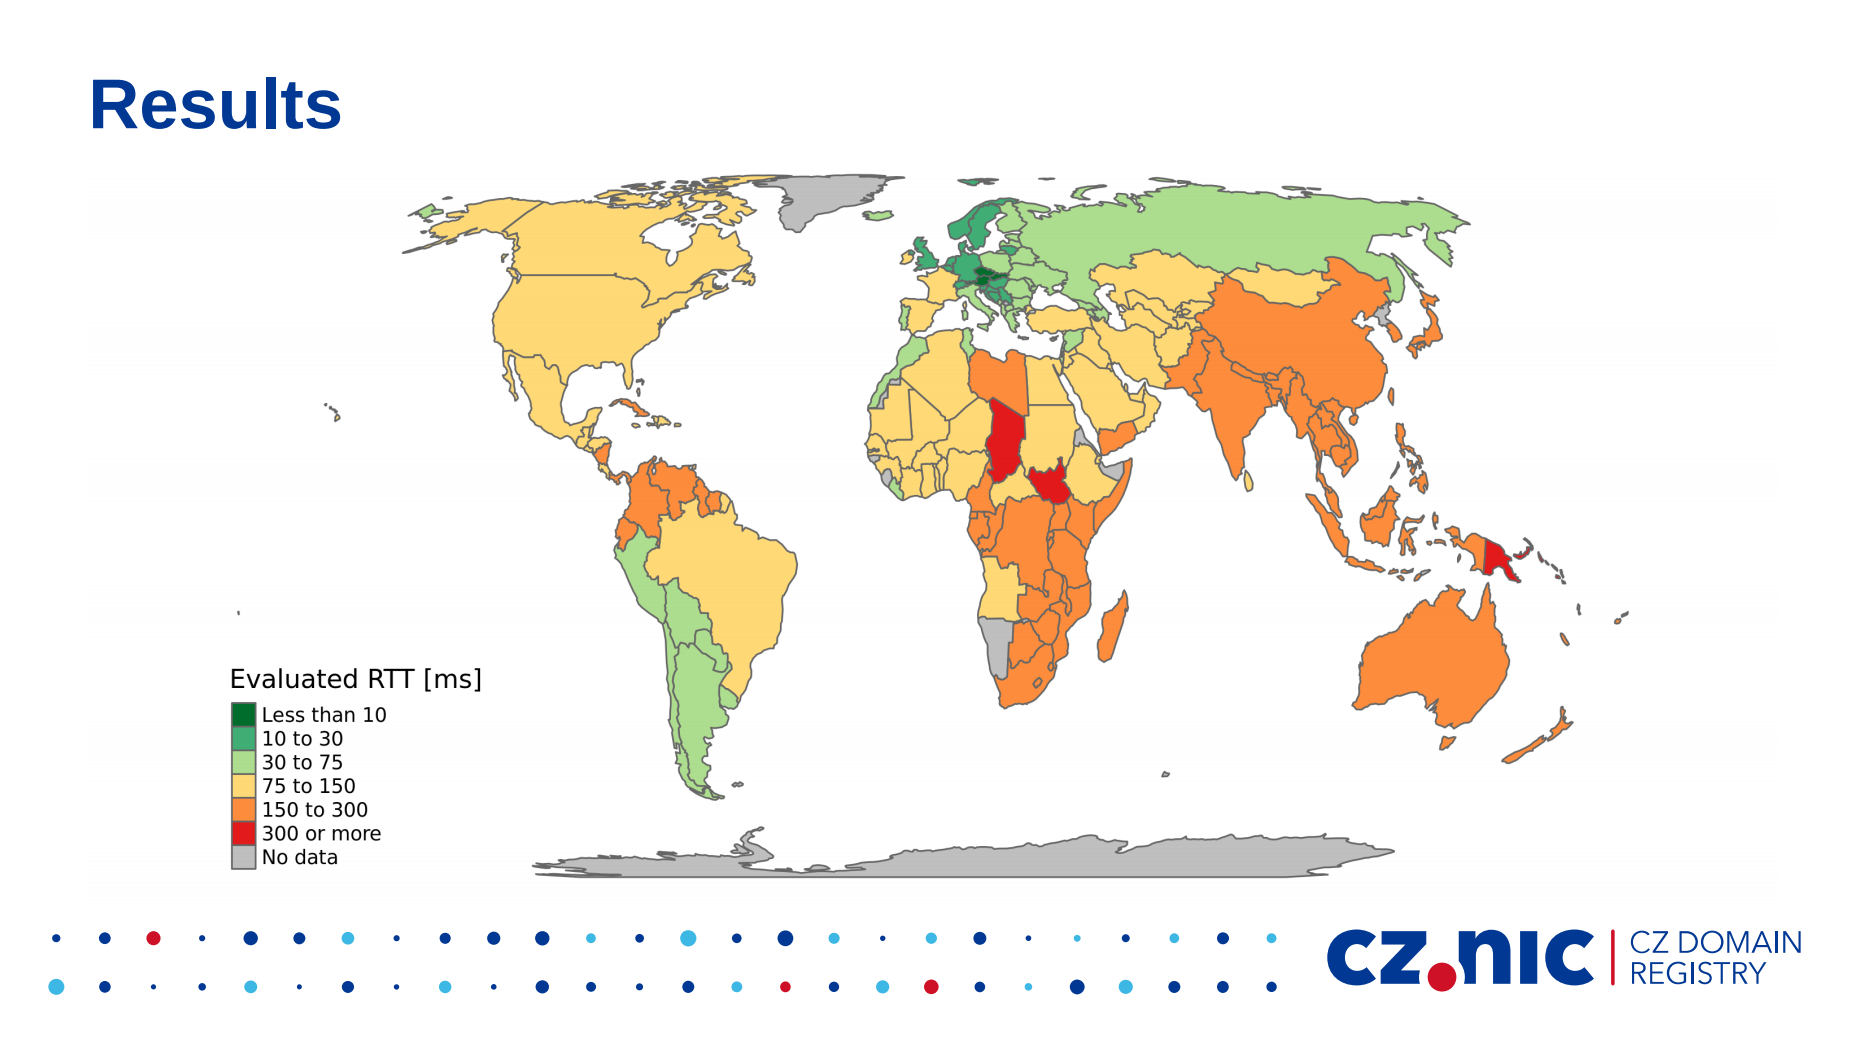
\includegraphics[width=1\textwidth]{images/maciej_globe.png}
   \caption{Ukázka z~analýzy Macieje Andzińského - pohled na vážený průměr RTT států (převzato z~\cite{cznic-maciej})}
     \label{fig:rttTCP}
\end{figure}

Následující otázka nevychází z~předešlé analýzy, ale odpověď na ni přinesou informace o~některých kvalitativních parametrech. Jak je rozdělen provoz mezi jednotlivé anycasty?


\subsection{Analýza dat}
Pro zodpovězení otázek byl použit kvantitavní výzkum nad daty od neděle 23. 2. 2020 do soboty 29. 2. 2020. V~období je zachycen jeden celý týdenní cyklus s~pracovními dny i víkendem a zároveň se v~týdnu nenacházely žádné státní svátky. Tato doba byla také vybrána z~důvodu, že nebyla pravděpodobně významně zatížena pandemií Covid-19. První potvrzené případy nákazy v~České republice byly prokázány 1. 3. 2020. \cite{covid-mzcr, covid-vlada}

Analýza dat byla prováděna nástrojem Jupyter Notebook s~Python knihovnami \texttt{matplotlib}, \texttt{pandas} a \texttt{numpy}. Celý postup je možné nalézt na  přiloženém paměťovém médiu.

Dříve než budou zodpovězeny výzkumné otázky je potřeba vysvětlit hodnotu, která se bude objevovat napříč celou analýzou a nenachází se \linebreak v~nasbíraných datech.  Jde o~hodnotu váženého RTT. Maciej Andziński tuto hodnotu označuje jako \textit{Evaluated RTT}. Jde o~propočítání váženého průměru RTT přes nějakou skupinu společných údajů, kde váhou je počet DNS dotazů po UDP. Tedy skupina s~větším celkovým počtem DNS dotazů bude mít větší váhu na RTT oproti těm tazatelům, kteří generují malý počet DNS dotazů. Skupinou například může být region a RTT je potom napočítáno pro všechny prvky takovéto skupiny (Afrika, Amerika, Asie, Evropa, Oceánie). Myšlenka s~váženým RTT je taková, že RTT u~tazatele DNS dotazu bude podobné po TCP i UDP. Vzorec pro vážené RTT je následující: 

\begin{equation}
\label{equ:RTT}
\overline{RTT_{i}} = \frac{\displaystyle\sum_{\forall j = i}^{Dataset}{RTT_j \cdot cnt_j}}{\displaystyle\sum_{\forall j = i}^{Dataset}{cnt_j}}, 
\forall i \in G, G \notin \emptyset
\end{equation}

$G$ ze vzorce \ref{equ:RTT} může být například neprázdná množina regionů (Afrika, Amerika, Asie, Evropa, Oceánie) a $i$ je jeden prvek z~množiny G. Dataset je množina všech řádků v~datovém souboru. RTT a cnt jsou sloupce v~datasetu, kde RTT je průměrné RTT a cnt je počet DNS dotazů.

Aby bylo možné zpracovat data ze 7 dní, bylo potřeba data agregovat v~každém dni podle serveru, verze IP protokolu, ASN, dvoupísmenného \linebreak označení státu, regionu, subregionu a anycastu. Jinými slovy byly odstraněny IP adresy, které jsou až moc velkým nijak potřebným detailem. Informace o~původcích dotazů jsou uchovány v~ASN, jménu státu a verzi IP protokolu. V~rámci agregace byly hodnoty průměrné RTT, vážené průměrné RTT a počet DNS dotazů napočítány následujícím způsobem: 

\begin{itemize}
	\item Průměrné RTT: aritmetický průměr
	\item Vážené průměrné RTT: průměr dle vzorce \ref{equ:RTT}
	\item Počet DNS dotazů: suma všech DNS dotazů
\end{itemize}

Jako první bude zodpovězena otázka týkající se rozdělení provozu přes jednotlivé anycasty.
Vzhledem k~tomu, že chování anycastů může být rozdílné pro IPv4 a IPv6, bylo nejdříve zjištěno, jaké je rozdělení provozu mezi jednotlivé verze internetového protokolu. DNS dotazy po IPv4 tvoří 72 \% provozu celé české domény. Provoz po IPv6 činí tedy 28 \%. Pro zjištění rozdělení provozu anycastu, byly dotazy seskupeny podle sloupce verze IP protokolu a použitého anycastu. Pro lepší čitelnost byla výsledná seskupení ještě rozdělena do dvou tabulek podle verze použitého IP. Výsledné rozdělení anycastu pro protokoly IPv4 a IPv6 lze vidět v~tabulkách \ref{tab:anycast4} a \ref{tab:anycast6}.

\begin{table}
\centering
\begin{tabular}{lrrrr}
\toprule
{anycast} &  \makecell{Průměrné\\RTT [ms]} &  \makecell{Vážené průměrné\\RTT [ms]} &  Počet dotazů &  \makecell{Podíl dotazů\\\ [\%]} \\
\midrule
A~& 117 & 26 &  1.598006e+09 & 22.86 \\
B & 107 & 16 &  1.904351e+09 & 27.25 \\
C & 129 & 17 &  1.597618e+09 & 22.86 \\
D & 110 & 16 &  1.889624e+09 & 27.03 \\
\bottomrule
\end{tabular}
 	\caption[]{Rozdělení DNS provozu po \textbf{IPv4} mezi jednotlivé anycasty} 
 	\label{tab:anycast4}
\end{table}

\begin{table}
\centering
\begin{tabular}{lrrrr}
\toprule
{anycast} &  \makecell{Průměrné\\RTT [ms]} &  \makecell{Vážené průměrné\\RTT [ms]} &  Počet dotazů &  \makecell{Podíl dotazů\\\ [\%]} \\
\midrule
A~& NaN & 0 & 618906975 & 22.90 \\
B & NaN & 0 & 710115132 & 26.28 \\
C & NaN & 0 & 714394517 & 26.43 \\
D & NaN & 0 & 659134565 & 24.39 \\

\bottomrule
\end{tabular}
 	\caption[]{Rozdělení DNS provozu po \textbf{IPv6} mezi jednotlivé anycasty} 
 	\label{tab:anycast6}
\end{table}

U~obou IP protokolů lze říci na základě procentuálního zastoupení, že rozdělení provozu je zhruba rovnoměrné. Všechny hodnoty se pohybují okolo 25 \% pro 4 anycasty. Na základě tabulky \ref{tab:anycast6}, popisující anycasty IPv6, lze vidět, že DNS dotazy po TCP neprobíhají. Veškerý TCP provoz je prováděn po IPv4. U~tabulky s~IPv4 je možno si všimnout, že vážené průměrné RTT je u~anycastu A~vyšší oproti ostatním. Při rozepsání pouze A~anycastu a rozdělení provozu na regiony lze vidět v~tabulce \ref{tab:anycast_a4_region}, že vážené RTT je ovlivněno špatnou dostupností z~asijského regionu. Asijský region pro anycast A~tvoří 12 \% provozu, což není zanedbatelný podíl.  

\begin{table}
\centering
\begin{tabular}{lrrrr}
\toprule
{Region} & \makecell{Průměrné\\RTT [ms]} &  \makecell{Vážené průměrné\\RTT [ms]} &  Počet dotazů &  \makecell{Podíl dotazů\\\ [\%]} \\
\midrule
      Asie & 226 & 102 & 1.927871e+08 & 12.06 \\
   Oceanie & 311 &  58 & 1.263731e+07 & 0.79 \\
  Amerika & 131 &  43 & 3.822603e+08 & 23.92 \\
    Afrika & 176 &  28 & 9.089478e+06 & 0.57 \\
    Evropa &  40 &   5 & 1.001232e+09 & 62.66 \\
                                                
\bottomrule
\end{tabular}
 	\caption[]{Rozdělení DNS provozu mezi regiony \textbf{A~anycastu} po \textbf{IPv4}} 
 	\label{tab:anycast_a4_region}
\end{table}

Na základě tohoto zjištění se dostáváme k~prvním dvěma výzkumným otázkám. Jak vypadá aktuální situace v~regionech? Pokud je RTT v~nějakém regionu horší oproti průměru celé české domény, lze to nějakým způsobem řešit? Odpověď na první otázku byla již částečně zodpovězena neboť, rozdělení provozu je momentálně známo pouze pro A~anycast. Další kroky analýzy budou zaměřeny na celý DNS provoz nehledě na anycasty a verze internetového protokolu. 

Po rozepsání DNS provozu celé CZ domény (tabulka \ref{tab:anycast_region}) lze vidět, že podíl asijského regionu na provozu se nijak výrazně neliší. Zásadně kleslo vážené RTT, které je i přesto oproti ostatním výrazně větší. Vážené průměrné RTT celé české domény je 13 ms. RTT pro asijský region je 56 ms, což je více než čtyřnásobek váženého průměru RTT celé české domény.

\begin{table}
\centering
\begin{tabular}{lrrrr}
\toprule
{Region} & \makecell{Průměrné\\RTT [ms]} &  \makecell{Vážené průměrné\\RTT [ms]} &  Počet dotazů &  \makecell{Podíl dotazů\\\ [\%]} \\
\midrule
Asie     & 226 & 56 &  1.112129e+09 & 11.47 \\
Oceanie  & 299 & 23 &  1.011141e+08 &  1.04 \\
Afrika   & 186 & 20 &  3.957741e+07 &  0.41 \\
Amerika & 124 & 15 &  3.014844e+09 & 31.11 \\
Evropa   &  48 &  4 &  5.424486e+09 & 55.97 \\
\bottomrule
\end{tabular}
 	\caption[]{Rozdělení DNS provozu CZ domény mezi regiony} 
 	\label{tab:anycast_region}
\end{table}

Region Asie se na celkovém provozu podílí zhruba 11.5 \%. Jde o~nezanedbatelný podíl v~provozu, který by bylo vhodné vylepšit. Možnosti, jak vylepšit dostupnost CZ domény v~asijském regionu, jsou v~zásadě dvě. První je vybudovat novou DNS lokalitu s~jedním či více DNS servery co nejblíže významným zdrojům dotazů. Druhou možností je navázat peeringová spojení v~již vybudovaných lokalitách. Vyvstávají tedy nové otázky. Kde je nejvýhodnější na základě aktuálního provozu vybudovat novou lokalitu? S~kým by měl být navázán peering s~jakými AS? 

Nejdříve se autor zaměřil na detailnější lokalizaci původce DNS dotazů a analyzoval nejvhodnější místo pro vybudování nové lokality. Při rozepsání DNS dotazů na subregiony (tabulka \ref{tab:anycast_subregion}) lze vidět, že nejhorší RTT (73 ms) a zároveň nejvíce dotazů (6.5 \%) z~celého asijského regionu je produkováno v~subregionu východní Asie. Oproti tomu západní a střední Asie mají průměrné vážené RTT pohybující se okolo průměru váženého RTT pro celou českou doménu a počet dotazů, které vygenerují se pohybuje okolo 1 \% z~celého provozu. V~těchto subregionech vybudování nové DNS lokality nebude mít takový vliv jako, kdyby nová lokalita byla  vybudována ve zbylých regionech Asie, kterými jsou východní, jihovýchodní a jižní Asie.  

\begin{table}
\centering
\begin{tabular}{lrr}
\toprule
{Subregion} & \makecell{Vážené průměrné\\RTT [ms]}  & \makecell{Podíl dotazů\\\ [\%]} \\
\midrule
Mikronésie                      & 104 &   0.003 \\
Východní Asie                    &  73 &   6.541 \\
Malajsie                       &  41 &   0.005 \\
Polynésie                       &  40 &   0.002 \\
Jihovýchodní Asie              &  38 &   3.162 \\
Jižní Asie                   &  35 &   1.004 \\
Austrálie a Nový Zéland       &  23 &   1.033 \\
Subsaharská Afrika              &  22 &   0.332 \\
Západní Asie                    &  18 &   0.695 \\
Severní Amerika                &  16 &  27.390 \\
Střední Asie                    &  15 &   0.074 \\
Severní Afrika                  &  11 &   0.077 \\
Jižní Evropa                    &  11 &   1.478 \\
Latinská Amerika a Karibik      &   8 &   3.716 \\
Západní Evropa                  &   5 &  14.139 \\
Severní Evropa                 &   4 &   9.537 \\
Východní Evropa                  &   2 &  30.814 \\
\bottomrule
\end{tabular}
 	\caption[]{Rozdělení DNS provozu CZ domény mezi subregiony} 
 	\label{tab:anycast_subregion}
\end{table}

Po zúžení výběru z~vybraných regionů je možno vidět, které státy generují největší procento provozu. Díky tomu si lze povšimnout, že většina provozu je generována ze států okolo Jihočínského moře. Dohromady těchto 10 států z~tabulky \ref{tab:anycast_asia_states} vyprodukuje 96 \% ze subregionů východní, jihovýchodní a jižní Asie. Zaměřením se na těchto 10 států bude pokryt skoro celý provoz z~těchto subregionů.   

\begin{table}
\centering
\begin{tabular}{lrrr}
\toprule
           Stát  &  \makecell{Vážené\\průměrné\\RTT [ms]} &  Počet dotazů &  \makecell{Podíl dotazů\\\ [\%]} \\
\midrule
                    Čína &  93 & 316376521 & 30.49 \\
               Singapure &  39 & 201501647 & 19.42 \\
Taiwan, Čínská provincie &  33 & 104988485 & 10.12 \\
                Japonsko &  26 &  90479568 &  8.72 \\
                   Indie &  33 &  81014102 &  7.81 \\
               Hong Kong &  49 &  76155161 &  7.34 \\
               Indonésie &  33 &  46214673 &  4.45 \\
      Korejská republika & 163 &  44327477 &  4.27 \\
                 Thajsko &  26 &  25202032 &  2.43 \\
                 Vietnam &  62 &  17806155 &  1.72 \\

\bottomrule
\end{tabular}
 	\caption[]{10 států z~východní, jihovýchodní a jižní Asie s~největším počtem dotazů na CZ doménu} 
 	\label{tab:anycast_asia_states}
\end{table}
 
Nyní je známo, odkud DNS provoz pochází. Kdo jej ale odbavuje? V~Japonsku má sdružení CZ.NIC jeden standalone DNS server, který odbavuje 17 \% provozu z~těchto 3 regionů. Většina tohoto provozu je ale odbavena v~evropských lokalitách celkem 66 \%. S~pomocí veřejně dostupné databáze PeeringDB lze jít do detailu a určit jaké veřejné peeringové uzly jsou nejvhodnější pro vybudování nové lokality. Výběr bude proveden na základě ASN. Výběr nové lokality by bylo nejlepší provést na  základě směrovacích tabulek peeringových uzlů. Tyto záznamy ale nejsou veřejně dostupné, proto k~výběru budou využity datové záznamy o~ASN z~nasbíraných dat a csv soubor, který byl vytvořen autorem této diplomové práce obsahující ASN v~jednotlivých veřejných peeringových uzlech. Dříve než bude vybírán vhodný peeringový uzel, je potřeba vybrat ty záznamy s~ASN, které pocházejí ze zmíněných subregionů. V~rámci zachování ochrany osobních údajů budou v~této práci zobrazované záznamy s~ASN anonymizovány. 

V~tabulce \ref{tab:anycast_asia_asn} je vypsáno 10 AS s~nejvíce DNS dotazy společně se zeměmi původu. Dohromady těchto 10 AS generuje 48 \% z~vybraných asijských regionů. Bylo by tedy vhodné zaměřit se na to, aby tato ASN byla v~peeringovém uzlu, ve kterém by sdružení CZ.NIC vybudovala novou DNS lokalitu. Také si je možné všimnout, že státy uvedené v~tabulce, vyjma Indie, se nacházejí geograficky v~okolí Jihočínského moře.

\begin{table}
\centering
\begin{tabular}{lrrrr}
\toprule
     ASN  &  Stát  &  \makecell{Vážené\\průměrné\\RTT [ms]} &  \makecell{Počet\\dotazů} &  \makecell{Podíl\\dotazů\\\ [\%]} \\
\midrule
ASN01  &                  Singapure &  41 &   135138818 &       13.02 \\ 
ASN02   &                      Čína &  69 &   115953141 &      11.17 \\ 
ASN03   &  Taiwan, Provincie Číny &  31 &    52498138 &       5.06 \\ 
ASN01  &                  Hong Kong &  53 &    49152912 &        4.74 \\ 
ASN01  &  Taiwan, Provincie Číny &  31 &    46290916 &        4.46 \\ 
ASN04   &                      Čína & 118 &    34236857 &       3.30 \\ 
ASN01   &                      Indie &  75 &    21198210 &       2.04 \\ 
ASN05 &                  Singapure &  99 &    20046697 &         1.93 \\ 
ASN06   &                      Čína &  32 &    18814507 &       1.81 \\ 
ASN07   &                      Čína & 193 &    17045509 &       1.64 \\

\bottomrule
\end{tabular}
 	\caption[]{10 ASN z~východní, jihovýchodní a jižní Asie s~největším počtem dotazů na CZ doménu} 
 	\label{tab:anycast_asia_asn}
\end{table}


Po spojení informací o~ASN v~jednotlivých peeringových uzlech a všech AS, která generují nějaký provoz ze zmíněných asijských subregionů, dostáváme tabulku \ref{tab:anycast_node_asn}. V~tabulce sloupec \textit{Hypotetický počet dotazů} popisuje kolik dotazů by teoreticky mohlo být odbaveno v~případě, že by provoz z~východní, jižní a jihovýchodní Asie byl celý odbavován v~peeringovém uzlu. Sloupec \textit{ASN} popisuje počet společných ASN v~dané lokalitě, se kterými by mohl být navázán peering. Hodnoty popisují AS, od kterých jde provoz na .cz doménu, nacházejí se ve specifikované oblasti a zároveň se nacházejí v~daném peeringovém uzlu. V~tabulce se nachází lokalita DE-CIX Frankfurt, ve které CZ.NIC provozuje své DNS servery. Hodnoty ve sloupcích \textit{ASN} a \textit{Hypotetický počet dotazů} tuto skutečnost nijak nereflektují. 

\begin{table}
\centering
\begin{tabular}{lrr}
\toprule
     Veřejný propojovací uzel  &  \makecell{Hypotetický\\počet dotazů} &  \makecell{Počet\\ společných ASN} \\
\midrule
                  DE-CIX Frankfurt Peering LAN &  585000216 & 292 \\
                                        AMS-IX &  548835976 & 326 \\
                               LINX LON1: Main &  544419306 & 307 \\
                    CoreSite - Any2 California &  508756527 & 240 \\
                             Equinix Singapore &  473432029 & 396 \\
                   DE-CIX New York Peering LAN &  454619032 & 145 \\
                        HKIX: HKIX Peering LAN &  435735116 & 348 \\
                                  NetIX: NetIX &  431513241 &  66 \\
                              Equinix Miami IX &  431066583 & 141 \\
                             Equinix Palo Alto &  414515528 & 149 \\
                             Equinix Hong Kong &  399932505 & 237 \\
                                    BBIX Tokyo &  395332678 & 346 \\
                          JPNAP Tokyo: Peering &  384899130 & 232 \\
                                         NYIIX &  383968880 & 148 \\
                             SGIX: Peering LAN &  383873284 & 187 \\


\bottomrule
\end{tabular}
 	\caption[]{15 veřejných peeringových uzlů s~největším počtem hypoteticky odbavených DNS dotazů} 
 	\label{tab:anycast_node_asn}
\end{table}

Při zaměření pouze na ty AS, která produkují 48 \% provozu ve vybraných subregionech (tabulka \ref{tab:anycast_asia_asn}), dostáváme velice podobné lokality (tabulka \ref{tab:anycast_node_asn_top}). Tabulka má stejný popis sloupců a lokality DE-CIX Frankfurt jako tabulka \ref{tab:anycast_node_asn}. 

\begin{table}
\centering
\begin{tabular}{lrr}
\toprule
     Veřejný propojovací uzel  &  \makecell{Hypotetický\\počet dotazů} &  \makecell{Počet\\ společných ASN} \\
\midrule
DE-CIX Frankfurt Peering LAN &  439777057 & 14 \\
                      AMS-IX &  405356653 & 12 \\
             LINX LON1: Main &  405356653 & 12 \\
  CoreSite - Any2 California &  390923440 & 10 \\
 DE-CIX New York Peering LAN &  390923440 & 10 \\
            Equinix Miami IX &  378150234 &  8 \\
                NetIX: NetIX &  378150234 &  8 \\
           Equinix Singapore &  314695231 &  8 \\
      HKIX: HKIX Peering LAN &  309450271 & 13 \\
           Equinix Hong Kong &  296617497 &  9 \\
                  BBIX Tokyo &  295017058 & 11 \\
           Equinix Palo Alto &  295017058 & 11 \\
           NYIIX Los Angeles &  295017058 & 11 \\
              BBIX Singapore &  295017058 & 11 \\
              BBIX Hong Kong &  295017058 & 11 \\
\bottomrule
\end{tabular}
 	\caption[]{15 veřejných peeringových uzlů s~největším počtem hypoteticky
odbavených DNS dotazů se zaměřením pouze na významná AS (viz tabulka \ref{tab:anycast_asia_asn})} 
 	\label{tab:anycast_node_asn_top}
\end{table}

V~obou tabulkách jsou většinou podobné peeringové uzly. Kromě toho se tam nacházejí uzly, které nejsou situovány v~Asii, ale jsou tam evropské nebo americké peeringové uzly.  Tyto uzly ve finálním výběru bude nejlepší vyřadit a vybrat lokality geograficky umístěné v~Asii. 

Na základě rozdělení provozu anycastu je známo, že v~asijském regionu je A~anycast nejhorší. Jak provoz vypadá pro ostatní anycasty? Při vypsání jednotlivých IPv4 anycastů z~celého asijského regionu vidíme, že A~anycast je jednoznačně nejhorší (viz tabulka \ref{tab:anycast_asia_letters}). Rozepsáním IPv6 anycastu pro Asii bychom nezískali vážené RTT, neboť není TCP provoz po IPv6 . Na základě tohoto pozorování by bylo tedy vhodné v~nové lokalitě provozovat A~anycast a snížit tak jeho RTT v~asijském regionu.

\begin{table}
\centering
\begin{tabular}{lrrr}
\toprule
     Anycast  & \makecell{Vážené\\průměrné\\RTT [ms]} &  \makecell{Počet\\dotazů} &  \makecell{Počet\\dotazů\\\ [\%]} \\
\midrule
A~& 102 &   192787060 &         23.57 \\
B &  81 &   188060210 &         22.99 \\
D &  72 &   207157563 &         25.32 \\
C &  56 &   230064013 &         28.12 \\
\bottomrule
\end{tabular}
 	\caption[]{Rozdělení asijského provozu podle \textbf{IPv4} anycastů} 
 	\label{tab:anycast_asia_letters}
\end{table}


Tímto bylo zodpovězeno na základě statistických dat potencionální místo k~vybudování nové lokality. Není zodpovězena otázka jak vylepšit provoz aniž by musela být budována nová lokalita. Nabízí se možnost navázat peering v~již vybudovaných lokalitách s~AS, které mají špatné vážené průměrné RTT, generují nemalé množství provozu a nejsou součástí MPLA v~daném peeringovém uzlu. Seznam takovýchto ASN a lokalit byl získán z~dat podobným způsobem jako při zjišťování možných nových lokalit. Seznam pouze nebyl agregován podle veřejného peeringového uzlu, aby nedošlo ke ztrátě detailu, které AS by bylo vhodné posílit. Ukázku takového seznamu je možné vidět v~tabulce \ref{tab:anycast_improve}. ASN byla opět anonymizována. Tento seznam je následně nutné porovnat v~DNS lokalitách se směrovací tabulkou a zjistit, zda routy těchto AS jsou získány v~rámci MPLA nebo z~tranzitního spoje. V~druhém případě je vhodné s~takovými AS navázat peering.

\begin{table}
\centering
\begin{tabular}{lr}
\toprule
     Veřejný propojovací uzel  & ASN \\
\midrule
DE-CIX Frankfurt Peering LAN & ASN01      \\  
DE-CIX Frankfurt Peering LAN & ASN02       \\  
DE-CIX Frankfurt Peering LAN & ASN03       \\  
DE-CIX Frankfurt Peering LAN & ASN04       \\  
DE-CIX Frankfurt Peering LAN & ASN05       \\  
    IX.br (PTT.br) São Paulo & ASN06     \\  
        JPNAP Tokyo: Peering & ASN07       \\  
             LINX LON1: Main & ASN02       \\  
             LINX LON1: Main & ASN03       \\  
             LINX LON1: Main & ASN05       \\  
                   LINX LON2 & ASN01      \\  
                      MIX-IT & ASN01      \\  
 NIX.CZ: Public peering VLAN & ASN01      \\  
                      NIX.SK & ASN01      \\  
                         VIX & ASN05       \\
\bottomrule
\end{tabular}
 	\caption[]{Ukázka seznamu ASN z~asijského regionu se kterými by bylo vhodné navázat peering v~již vybudovaných DNS lokalitách} 
 	\label{tab:anycast_improve}
\end{table}




\section{Návrhy na zlepšení provozu DNS anycastu}
Na základě analýzy bylo zjištěno, že DNS anycast české domény je hůře dostupný z~regionu Asie, přesněji ze subregionů východní Asie, jižní Asie a jihovýchodní Asie. Aby bylo dosaženo zlepšení, autor práce navrhuje pokusit se v~prvé řadě navázat v~již vybudovaných DNS lokalitách CZ.NIC peering s~AS, které generují velké množství provozu, mají špatné RTT a provoz od nich jde přes tranzitivní spojení.

Druhým návrhem je vybudovat novou lokalitu v~okolí Jihočínského moře. Důvodem této oblasti je, že velké množství států, které produkují DNS provoz na CZ doménu, se nachází v~jeho okolí. Vybráním veřejného peeringového uzlu v~této oblasti může být velká část provozu stažena z~evropských DNS lokalit a tím snížena jejich zátěž. Lokalita by měla být vybrána ze seznamu uvedeného v~tabulce \ref{tab:anycast_node_asn_top}, která popisuje kolik by teoreticky odbavila provozu od AS s~největším počtem DNS dotazů.

Jelikož nejsou známy směrovací tabulky nelze určit, zda provoz z~nějakého státu bude skutečně stažen do nové lokality. Je zde ještě jeden faktor, který může být brán při výběru lokality v~potaz a který popisuje, jak spolu jednotlivé státy komunikují. Jde o~kabelové internetové propojení, přesněji řečeno podmořské kabelové připojení. Jak jsou internetové podmořské kabely vedeny, lze dohledat na několika webových portálech jedním takovým je například \textit{submarinecablemap.com}. Na tomto portálu je zobrazeno kudy jsou kabely vedeny a jaké lokality propojují. 

Předpokládejme, že veřejné peeringové uzly a datacentra jsou připojeny k~podmořským internetovým kabelům na základě toho že tyto kabely jsou vedeny tímto městem/lokalitou. Pokud bude tento předpoklad brán v~potaz, měla by být vybraná lokalita s~nějakým podmořským kabelem, který propojuje pokud možno všechny státy s~významným podílem na DNS dotazech na CZ anycasty. Vhodným zvolením lokality může být i zlepšen provoz z~Austrálie a Nového Zélandu, které generují okolo 1 \% z~provozu celé české domény. 

Na základě tabulky \ref{tab:anycast_asia_letters} by bylo vhodné v~nové lokalitě vybudovat A~anycast. 











%==========================================











\chapter{Program pro vizualizaci provozu DNS anycastu}
\section{Popis výchozího stavu a záměru}
Náhled na provoz DNS anycastu je v~současné době zajištěn pomocí síťových Weathermap postavených nad SNMP (Simple Network Management Protocol) a sběrem dat nástroji projektu ADAM. SNMP zobrazuje provoz v~reálném čase z~hlediska přenosové kapacity, zatížení linek. Oproti tomu nástroje projektu ADAM slouží pro hlubší statistickou analýzu provozu. Bohužel ani jeden z~nástrojů neumí zobrazit data v~reálném čase zároveň s~detailnější analýzou provozu DNS anycastů. Každý zvládá pouze jedno z~toho.

Programem pro vizualizaci provozu DNS anycastu je tedy myšlen takový program, který v~reálném čase zobrazí detailněji aktuální DNS provoz, respektive jeho nejdůležitější parametry. Bude schopen zobrazit počty dotazů, vytížení jednotlivých anycastů a latenci dotazů. Program by měl být také připraven na rozšíření o~funkcionality upozorňování neobvyklých událostí (alerting) a strojového učení. 

\section{Design monitoringu}
Návrh celé architektury vychází z~architektury MINDS (Minnesota Intrusion Detection System), který lze vidět na obrázku \ref{fig:minds}. Zachycená data jsou v~této architektuře uložena, filtrována a následně zpracována analytickými nástroji a metodami. Takto jsou již zpracována data DNS provozu pomocí nástrojů projektu ADAM. Přenos pcapů od DNS serverů na úložiště, jejich následné zpracování a nahrání do clusteru trvá až 24 hodin. Z~tohoto důvodu není vhodné tato data použít pro vizualizaci provozu, pokud je kladen důraz na aktuálnost vizualizovaných dat. \cite{minds}

\begin{figure}[ht]
  \centering
   \includegraphics[width=0.8\textwidth]{images/minds.png}
   \caption{Architektura MINDS (převzato z~\cite{minds})}
     \label{fig:minds}
\end{figure}

V~návrhu autorova monitoringu musí tedy být některé části prohozeny. Vhodným způsobem jak nejlépe zpracovávat pakety bude provádět filtraci již na samotných DNS serverech a následně sbírat a analyzovat jen vyfiltrované informace. To by mělo zajistit časovou úsporu, ale na druhé straně vyvstává několik problémů, které bude třeba reflektovat jak v~návrhu, tak v~implementaci. Prvním problémem je vytížení DNS serveru. Sběr dat nesmí být pro server nijak omezující a neměl by mít vliv na samotný běh DNS služby. Druhým problémem je, jak zajistit distribuci nasbíraných dat s~následnou vizualizací. Přenos dat musí být navíc prováděn na nezabezpečených linkách šifrovaně, jelikož budou přenášena citlivá a interní data. 

Nasbíraná a vyfiltrovaná data budou uložena pouze na RAM. Tím bude využito předností DNS serverů, kde jejich HW konfigurace je navržena na výpočetní výkon. Servery mnohdy nemají velkou diskovou kapacitu. Navíc má být vizualizován aktuální provoz a ukládání dat na disk a čtení zbytečně zabírá výpočetní čas. Mimo jiné neustálé operace čtení a zápis na disk snižují jeho životnost a výměna disku mimo Českou republiku je problematická.  

Pro přenos dat bude zvolen protokol HTTP, který zajistí kompatibilita napříč širokým spektrem programovacích jazyků. Jeho SSL rozšíření (HTTPS) vyřeší problém s~bezpečností dat. Pro distribuci nasbíraných dat bude zvolena komunikace od centrálního prvku k~DNS serverům. Centrálním prvkem je myšlen server, který bude sbírat data od všech DNS serverů a bude iniciátorem komunikace. Tento centrální prvek bude dále nazýván jako \texttt{Collector}. Aplikace běžící na DNS serveru, která zpracovává provoz a poskytuje nasbíraná data, bude nazývána jako sonda (\textit{anglicky probe}). Výhodou této centralizace bude jednoduší administrace všech prvků. Tento model sběru dat a následná vizualizace jsou zachyceny v~obrázku \ref{fig:monitoring}. 

\begin{figure}[ht]
  \centering
   \includegraphics[width=0.8\textwidth]{images/monitoring.pdf}
   \caption{Monitoring standalone serveru}
     \label{fig:monitoring}
\end{figure}


Sběr dat \texttt{Collectorem} ze sondy běžící na standalone DNS serverech je jednodušší oproti sondám běžícím v~DNS stacku. Standalone DNS servery mají 2 rozhraní s~veřejnými adresami. Dotazy na nasbíraná data mohou tak probíhat napřímo. Ukázku sondy na standalone DNS serveru přes OOB rozhraní lze vidět na obrázku \ref{fig:monitor-standalone}. 


\begin{figure}[ht]
  \centering
   \includegraphics[width=0.6\textwidth]{images/monitoring-standalone.pdf}
   \caption{Model sběru dat na standalone DNS serveru}
     \label{fig:monitor-standalone}
\end{figure}

Pro sběr dat z~DNS stacku bude využit management server, kde bude běžet aplikace, která bude redistribuovat HTTPS dotazy od \texttt{Collectoru} na jednotlivé sondy. Taková aplikace bude označována jako \texttt{Middleware} a bude implementována na management serveru. Důvodů pro volbu management serveru vůči gateway směrovači je více. Jedním z~důvodů je, že DNS provoz jde přes gateway směrovač a ten je vytížen směrovacím démonem a samotným provozem. Hlavním důvodem je ale to, že management server je v~infrastrukturách DNS stacků (viz obrázky \ref{fig:infra-30stack} a \ref{fig:infra-3stack}) vždy linuxový server. Ve stacku o~30 DNS serverech je gateway směrovač CISCO, Juniper nebo jiné síťové zařízení. Tím bude zajištěno, že nebude potřeba mít více verzí Middleware aplikací. Jak bude vypadat nasazený monitoring na jednom DNS stacku o~3 DNS serverech je popsáno v~obrázku \ref{fig:monitor-3stack}. V~obrázku jsou zachyceny pouze prvky infrastruktury stacku, které bude monitoring využívat. 

\begin{figure}[ht]
  \centering
   \includegraphics[width=0.5\textwidth]{images/monitoring-3stack.pdf}
   \caption{Monitoring stacku o~3 serverech}
     \label{fig:monitor-3stack}
\end{figure}





\section{Implementace}
Jako programovací jazyk byl zvolen Python kvůli velké škále modulů, které nabízí.  Zároveň jsou moduly Pythonu napsány v~jazyce C, takže je předpoklad, že veškeré části budou dostatečně rychlé. Základními stavebními kameny na kterých je celý monitoring postaven jsou Python moduly \texttt{scapy}, \texttt{django} a \texttt{flask}. Poslední dva moduly jsou webovými frameworky a scapy je modul pro zachytávání a odposlouchávání síťového provozu. 

Celý monitoring je navržen tak, že snímá úhrn dotazů za určité časové období. Data jsou zaznamenávána na sondě do té doby než přijde příslušný dotaz z~\texttt{Collectoru} nebo \texttt{Middleware}. Sonda po obdržení dotazu odešle zpět tazateli data opatřená časovou známkou označující dobu, kdy sonda tento dotaz přijala. Nasbíraná data jsou na sondě smazána a sběr informací z~provozu začíná od začátku.

\subsection{Sonda}
Program sondy nese název \texttt{dns-sniffer} a její implementace byla napsána v~Pythonu ve verzi 3.5. Volba této verza byla z~toho důvodu, že některé DNS servery běží na operačním systému Debian 9 (v~době vývoje podporovaný), který má v~repositářích poslední stabilní verzi Pythonu 3.5.3. Aby bylo dosaženo bezpečnosti a stability provozu sondy, autor se rozhodl instalovat pouze balíčky, které jsou v~oficiálních repositářích a tím neohrozil provoz DNS serverů. Bezpečnostní či jiná chyba v~Pythonu a následné omezení běhu více DNS serverů by mohly mít negativní vliv na provoz celé CZ. domény.

Sonda byla naimplementována jako dvouvláknová aplikace. Jedno vlákno pro odposlech provozu na síťovém rozhraní a druhé pro obsluhu HTTP(S) dotazů. Obě vlákna mají přístup k~proměnné, do které se zaznamenávají relevantní informace o~provozu. V~případě dotazu HTTP(S) na obsah nasbíraných dat je tato proměnná přečtena a vrácena v~odpovědi. Přístupy k~této proměnné jsou opatřeny vláknovými zámky a tím je ošetřena kritická sekce paměti.

\subsubsection{API}
Jako webový framework pro API je zde použit \texttt{flask}. Jeho struktura i použití je jednoduché. API by se dalo rozdělit do dvou skupin. První skupina je určena pro manipulaci s~nasbíranými daty a druhá pro nastavení sběru dat, přesněji řečeno nastavení pro jaké anycasty se má dělat detailnější sběr dat. 

Každý dotaz na cílovou cestu (routu) je přijat jen v~případě, že obsahuje v~hlavičce \texttt{Content-type: application/json}. Veškerá data, která aplikace přijímá, musí být v~JSON formátu. V~každé odpovědi je identifikace serveru, z~jaké lokace data pochází a zároveň odpověď obsahuje v~kolik sonda dotaz obdržela. Identita lokace a serveru je brána ze jména hostitelského DNS serveru. 

Cesta \texttt{/} přijímá dvě HTTP(S) metody, a to \texttt{GET} a \texttt{DELETE}. Obě metody vrací data, která sonda nasbírala. Rozdíl mezi nimi je ten, že metoda \texttt{DELETE} nasbírané informace zároveň i smaže. Dotaz na sondu a následná odpověď může vypadat následovně. 

\begin{verbatim}
curl http://example-probe.cz -X GET
{  "dns":"linux-server",
"timestamp":"2020-04-01 15:52:51",
"location":"linux-server",
"traffic":{    "xxx.xxx.xxx.xxx":{      
  "RTT_min":30,
  "RTT_sum":30,
  "RTT_queries":1,
  "RTT_max":30,
  "queries":1,
  "anycast":{
    "a4":1,
    "a6":0    
}}}}
\end{verbatim}

Druhá skupina obsahuje cesty dvě. \texttt{/config} a \texttt{/configDel}. Každá \texttt{DELETE} a \texttt{POST} metoda má vedlejší efekt ten, že smaže aktuální nasbíraná data. \linebreak \texttt{configDel} obsahuje pouze metodu \texttt{DELETE} a jejím účelem je smazat celou konfiguraci anycastu na sondě. 

Cesta \texttt{/config} odpovídá na tři metody \texttt{GET}, \texttt{POST} a \texttt{DELETE}. První metoda pouze vrací aktuální konfiguraci. \texttt{POST} metoda zkontroluje příchozí JSON obsahující, informace o~nastavení anycastů a v~případě správného formátu je stará konfigurace přemazána aktuálně příchozí. Formát takového JSONu může vypadat takto:

\begin{verbatim}
{  "anycast":{
"a":{
  "ipv4":"xxx.xxx.xxx.xxx",
  "ipv6":"xxxx:xxxx::x"
},
"b":{
  "ipv4":"xxx.xxx.xxx.xxy",
  "ipv6":"xxxx:xxxx::y"
},
"c":{
  "ipv4":"xxx.xxx.xxx.xxz",
  "ipv6":"xxxx:xxxx::z"
}}}
\end{verbatim}

Písmena \textit{a}, \textit{b} a \textit{c} označují o~jaký anycast se jedná, respektive jeho pojmenování. Toto jméno je pak reflektováno v~odpovědi( viz předešlá ukázka \texttt{curl} dotazu a odpovědi), kde \texttt{a4} a \texttt{a6} jsou složeninou názvu anycastu a o~jakou verzi internetového protokolu se jednalo. 

Poslední metodou je metoda \texttt{DELETE}, která maže nastavení anycastu podle jeho jména. Vstupní JSON ve formátu (ukázka níže) smaže z~nastavení anycasty pojmenované \textit{b} a \textit{c}.
\begin{verbatim}
{
"anycast":[
"b", "c"
]}
\end{verbatim}




\subsubsection{Sběr dat}
Odposlech provozu na rozhraní a následná filtrace informací probíhá v~samostatném vláknu. Vlákno je spuštěno po načtení frameworku \texttt{flask} a následně je spuštěna metoda \texttt{sniff}, která je součástí Python modulu \texttt{scapy}. Modul scapy byl autorem vybrán na základě předešlé zkušenosti z~předmětu \texttt{MI-SIB}.

Metoda \texttt{sniff} poslouchá v~nekonečné smyčce na síťovém rozhraní, které je specifikováno v~konfiguračním souboru. Na každý paket procházející tímto rozhraním je aplikován filtr, který je více popsán v~kapitole \textit{\nameref{sec:filter}}. Výchozím chováním metody \texttt{sniff} je uchovávat veškeré zachycené pakety v~paměti. Tuto volbu bylo potřeba vypnout, aby se tím nezahlcovala RAM DNS serveru a program tak nevypotřeboval veškerou dostupnou paměť. Toto chování lze vypnout pomocí parametru \texttt{store}, který se nastaví na 0. 

 
\subsubsection{Filtrace a formát dat}
\label{sec:filter}
%\label{sec:jsonStructure}
Data programu uchovávaná v~RAM musí být dostatečně malá, aby objem dat nepřekročil paměťovou kapacitu serveru i v~případě DDOS útoku. Z~dat jsou tedy vybrány jen relevantní informace z~provozu, kde klíčem záznamů je IP adresa a k~ní přidružené hodnoty:
\begin{itemize}
	\item Počet dotazů
	\item Počet RTT dotazů
	\item Suma RTT všech dotazů
	\item Maximální hodnota RTT
	\item Minimální hodnota RTT
	\item Rozdělení počtu dotazů přes anycasty
\end{itemize}


Bylo třeba vyřešit problém s~omezenou kapacitou pro sbíraná data. Zásadní pro tuto úsporu byla volba tzv. úhrnného sběru dat. Není sbíráno v~jakém okamžiku paket dorazil, ale pouze že dorazil v~určité časové periodě. Celý sběr dat je založen na navyšování počítadel a není postaven na nedeterministických informacích. Z~příchozího paketu se zjistí na jaký anycast dotaz mířil, poznamená se zda se jednalo o~IPv4 nebo IPv6, a pokud se jednalo o~dotaz po TCP vypočítá se z~předešlého \textit{tree way handshake} procesu RTT. Veškeré informace jsou uloženy pro jednu IP adresu a pokud by se sbíraly nedeterministické informace z~dotazů jednoduše by mohlo docházet k~situacím, kdy bude touto aplikací využita veškerá dostupná RAM. Nedeterministickými informacemi jsou myšlena třeba jména dotazovaných domén. Z~kapacitních důvodů není možné uchovávat ke každé IP adrese všechna jména dotazovaných domén. Jenom existujících doménových jmen je ke dni 20. 4. 2020 1 356 308. \cite{cznic-statistics}

Data jsou ukládána v~Pythonu do slovníku, \texttt{dict}, kde klíčem je IP adresa a jako hodnota je další slovník, který obsahuje jednotlivé položky popsané v~listu výše. Důvod proč je zvolena tato datová struktura je jednoduchá konverze do JSON formát a není tedy nutné složitě konvertovat data. Struktura v~JSONu může vypadat takto: 


\begin{verbatim}

{
"dns":"probe01",
"location":"probe01",
"timestamp":"2020-04-01 17:32:15",
"traffic":{
  "xxx.xxx.xxx.xxy":{
    "queries":13,
    "RTT_sum":48,
    "RTT_queries":2,
    "RTT_min":32,
    "RTT_max":16,
    "anycast":{
    "a4": 13,
    "a6": 0
}}}}
\end{verbatim}

Výpočet počtu dotazů je pouze zvýšení hodnoty o~jedna pro příchozí jeden paket. RTT je potřeba propočítat přes více příchozích a odchozích paketů. Pokud sonda zaznamená příchozí TCP packet s~příznakem SYN, jsou do paměti programu uloženy  zdrojová adresa a zdrojový port. Čas odchozího paketu s~příznaky SYN a ACK se uloží do již vytvořené proměnné k~dalšímu využití. Z~následné odpovědi od klienta s~příznakem ACK je získán čas, od kterého je odečten čas předchozího paketu s~příznaky SYN a ACK.

Zdrojová adresa a port jsou ukládány do slovníku jako jeden klíč a hodnota je potom naměřený čas. Čas je brán z~třídy packet, která obsahuje metodu \texttt{time}. Tato metoda vrací čas v~sekundách. Čas, který je zaznamenán, je převeden na milisekundy a zaokrouhlen na celá čísla. V~programu bylo myšleno i na možný TCP SYN flood útok. V~případě že by útočník útočil vždy z~jiného zdrojového portu, plnil by obsah paměti programu velkým množstvím záznamů. Pro takový případ je v~programu mechanismus, který v~případě většího množství navázaných spojení než je povolený limit, odstraňuje záznamy podle principu FIFO (First In First Out). Tento limit lze nastavit v~konfiguračním souboru.

\subsubsection{Konfigurace}
\label{sec:probeConf}
Konfigurace samotného programu je uložena v~souboru \texttt{dns-sniffer.conf}, který je očekáván ve složce \texttt{/etc/dns-sniffer/}. V~souboru se nastavuje na jakém síťovém rozhraní se bude poslouchat, limit navázaných TCP spojení, jméno a heslo uživatele, které slouží pro autentizaci a autorizaci v~aplikaci. Tato konfigurace je vždy načtena při startu nebo restartu programu. Jedná se o~\texttt{.ini} formát a konfigurace může vypadat následovně: 

\begin{verbatim}
[settings]
interface=eth0
rtt_candidates_size=101

[user]
name=honza
password=honza
\end{verbatim}

Pokud nejsou nastaveny zároveň volby \texttt{name} a \texttt{password} autentizace a autorizace pomocí jména a hesla není zapnuta. Jak má vypadat zpráva pro API s~autentizací a autorizací je ukázáno v~kapitole \nameref{sec:security}. Výchozí hodnota \texttt{rtt\_candidates\_size} je 100. Volba \texttt{interface} nemá výchozí hodnotu, jelikož se jedná o~stěžejní informaci. Pokud není nastaveno síťové rozhraní, na kterém má sonda poslouchat, poslouchání vůbec nezačne. 

Je zde ještě konfigurace, kterou lze měnit za běhu pomocí API. Jedná se o~nastavení anycastů, na kterých daný DNS server poslouchá. Konfigurace je uložena v~souboru \texttt{dns-sniffer\_startup.conf} ve stejné složce jako soubor výše. Obsah je ve stejné podobě v~jaké byla konfigurace obdržena pomocí POST metody pro cestu \texttt{/config}. Uložený obsah je tedy také v~JSON formátu. Druhý konfigurační soubor vznikl proto, aby vyřešil problém, kdy aplikace spadne a ztratí nastavení, které bylo přijato za běhu programu. Tento konfigurační soubor, pokud existuje, eliminuje ztráty informací z~provozu po restartování aplikace. Přijde-li zmíněný POST dotaz, soubor neexistuje a program má práva pro vytvoření souboru ve složce \texttt{/etc/dns-sniffer/}, bude tento konfigurační soubor vytvořen. 

\subsection{Middleware}
Druhou částí monitoringu je aplikace middleware, která nese název \linebreak \texttt{dns-middleware}. Hlavní funkcí této aplikace je redistribuce dotazů od \linebreak \texttt{Collectoru} sondám. Dotaz obdržený od \texttt{Collectoru} je přeposlán na každou sondu, kterou má middleware uvedenu v~konfiguraci. Následné odpovědi od sond jsou dány do jedné odpovědi, která je poslána zpět \texttt{Collectoru}. 

Implementace a kód jsou velice podobné sondě. Byly zde použity stejné stavební kameny s~tím rozdílem, že zde není použit modul \texttt{scapy}. Middleware je ze stejného důvodu jako sonda postaven na Pythonu 3.5.3 (Debian 9, bezpečnost a kompatibilita). Aplikace je jednovláknová a jednotlivé HTTP(S) dotazy na sondy probíhají sekvenčně. Není tedy pro každou sondu nebo skupinu sond vytvořeno nové vlákno, které zajistí ze sond sběr dat. 

\subsubsection{API}
API je postaveno nad webovým frameworkem \texttt{flask}. Dotazy jsou přijímány na cílovou cestu (routu) jen v~případě, že dotaz obsahuje v~hlavičce \texttt{Content-type: application/json}. Na začátku každého dotazu na existující cílovou cestu je ověřeno, že dotazovaný má potřebné informace pro autentizaci a autorizaci je-li zapnuto. Cesty se dají rozdělit na dvě skupiny. První skupina se váže ke konfiguraci sond na middlewaru a druhá je skupina cest, které jsou na sondy přeposlány.

V~první skupině existují dvě cesty \texttt{/probes} a \texttt{/deleteProbes}. Druhá zmíněná cesta za pomocí \texttt{DELETE} metody smaže celé nastavení sond. Cesta \texttt{/probes} obsahuje dvě metody \texttt{GET} a \texttt{POST}. \texttt{GET} vrací aktuální konfiguraci sond, která obsahuje jak jsou sondy pojmenovány a jak mají nastaveny IPv4 a IPv6 adresy viz níže.  
\begin{verbatim}
curl https://middleware.cz/probes -X GET
{  "probe01":{
"ipv4":"xxx.xxx.xxx.xxx",
"ipv6":"xxxx:xxxx::x"
},
"probe02":{
"ipv4":"",
"ipv6":"xxxx:xxxx::y"
}}
\end{verbatim}

\texttt{POST} dotaz nastavuje na jaké sondy má middleware dotazy od \texttt{Collectoru} přesměrovávat. V~dotazu jsou očekávána data v~podobě JSON formátu, který může vypadat například takto:
\begin{verbatim}
{  "probe01":{
"ipv4":"xxx.xxx.xxx.xxx",
"ipv6":"xxxx:xxxx::x"
},
"probe02":{
"ipv4":"",
"ipv6":"xxxx:xxxx::y"
}}
\end{verbatim}

Ve druhé skupině se nacházejí cesty \texttt{/} a \texttt{/config}. V~obou případech jsou příchozí dotazy na \texttt{middleware} přeposlány na všechny nastavené sondy pomocí protokolu HTTP \footnote{Popis důvodu pouze HTTP je popsán v~kapitole \nameref{sec:security}} a následně je od nich získaná odpověď odeslána zpět tazateli. Každý dotaz je poslán na sondu ve stejné podobě v~jaké ho obdržel \texttt{middleware}. To znamená, že je použita stejná cesta, metoda a obdržený JSON. Následná odpověď je pak vytvořena jako slovník (\texttt{dict}), kde klíč je název sondy a hodnota odpověď ze sondy. Obě cesty obsluhují metody \texttt{GET} a \texttt{DELETE}. Cesta \texttt{/config} pak ještě přeposílá dotazy, které přijdou s~metodou \texttt{POST}. Níže je ukázka, jak může vypadat taková odpověď. 

\begin{verbatim}
curl https://example.cz -X GET
{
"probe01":{
"dns":"probe01",
"location":"linux-middleware",
"timestamp":"2020-04-01 17:32:15",
"traffic":{
  "xxx.xxx.xxx.xxy":{
    "queries":4,
    "anycast":{
}}}},
"probe02":{
"location":"linux-middleware",
"timestamp":"2020-04-01 17:32:15",
"dns":"probe02",
"traffic":{
  "yyy.xxx.xxx.xxy":{
    "queries":13,
    "RTT_sum":48,
    "RTT_queries":2,
    "RTT_min":32,
    "RTT_max":16,
    "anycast":{      
}}},}}
\end{verbatim}

Veškerá data, která aplikace přijímá, musí být v~JSON formátu. V~každé odpovědi od sondy jsou v~hlavičce změněny údaje hodnoty \texttt{location} a \linebreak \texttt{timestamp}. Obě hodnoty jsou měněny z~důvodu jednoty záznamů. Hodnota \texttt{location} je změněna podle jména hostujícího serveru. Čas je měněn z~toho důvodu, že sondy nemusí odpovědět ve stejný okamžik. Aby bylo zřejmé, že data patří k~sobě a šlo nad nimi dělat dobře vizualizace, je čas změněn na hodnotu, kdy aplikace Middleware dotaz obdržela. 


\subsubsection{Konfigurace}
\label{sec:middleware-conf}
Konfigurace je zde dvojího druhu jako u~sondy. Konfigurace, která je načtena při startu a následně za běhu programu se nemění, je očekávána ve složce \texttt{/etc/dns-middleware}. Konfigurační soubor je ve formátu \texttt{.ini} a jeho jméno je \texttt{dns-middleware.conf}. Obsah souboru může vypadat takto: 
\begin{verbatim}
[settings]
timeout=10
retry=2

[user]
name=honza
password=honza
\end{verbatim}
Volby \texttt{name} a \texttt{password} slouží pro autentizaci a autorizaci. Pokud ani jedna z~těchto voleb není nastavena, nebude u~příchozích dotazů prováděna autentizace a autorizace. Jak má vypadat zpráva pro API s~autentizací a autorizací je ukázáno v~kapitole \nameref{sec:security}. \texttt{timeout} a \texttt{retry} jsou volby, které nastavují, jak bude navázáno spojení se sondami. První volba říká po jaké době bude spojení se sondou ukončeno, pokud sonda po X sekundách odpověděla middlewaru na dotaz. Hodnota musí být celé číslo a výchozí hodnota je nastavena na 5 sekund. Druhá volba nastavuje, kolikrát se v~případě neúspěšného dotazu Middleware pokusí sondy opět dotázat. Výchozí hodnota je 3. 


Druhý konfigurační soubor je také načten po startu programu s~tím \linebreak rozdílem, že tato konfigurace může být změněna za pomoci API. Jedná se o~POST dotaz na cestu \texttt{/probes}. JSON, který je posílán v~rámci tohoto dotazu, je uložen ve stejném formátu do tohoto druhého konfiguračního souboru. Tento soubor je pojmenován \texttt{dns-middleware\_startup.conf} a uložen do složky \texttt{/etc/dns-middleware}. Přijde-li zmíněný POST dotaz, soubor \linebreak neexistuje a program  má  práva pro vytvoření souboru ve složce \linebreak \texttt{/etc/dns-middleware/}, bude tento konfigurační soubor vytvořen. 

%%%% ====== ELastic 


\subsection{Vizualizační nástroj a uchování nasbíraných dat}
\label{sec:vizualizationStorage}

Nejdříve bylo potřeba vybrat vhodný open source nástroj pro uchovávání dat. Pro tuto činnost byl vybrán Elasticsearch. Elasticsearch je vysoce škálovatelný full-textový vyhledávač a analytický nástroj. Umožňuje vyhledávat, ukládat a analyzovat velké množství dat velice rychle skoro až v~reálném čase. Nejedná se o~relační databázi, ale NOSQL databázi a pro způsob komunikace využívá REST API založené na JSON formátu. Také obsahuje funkci, která po určité časové periodě uložená data automaticky promazává. Data starší než nastavená časová perioda mohou být z~databáze smazána. Tato funkce může ušetřit velké množství diskové paměti. \cite{elastic}

REST API založené na JSON formátech také ušetří mnoho výpočetního času, neboť data ze sond jsou sbírána také v~tomto formátu. V~\texttt{Collectoru} bude pouze potřeba každý záznam čítající IP adresu s~přidruženými informacemi jako počet dotazů, počet RTT dotazů atd., rozdělit a přidat hlavičku, která se nachází v~každé odpovědi a obsahuje časovou známku, DNS server a lokalitu. Tato konverze z~jednoho velkého datového celku na více samostatných částí je znázorněna v~obrázku \ref{fig:dataConversion}. 

\begin{figure}[ht]
	\centering
	\includegraphics[width=0.8\textwidth]{images/data-conversion.pdf}
   \caption{Konverze dat do formátu vhodného pro Elasticsearch}
	\label{fig:dataConversion}
\end{figure}

Data se do databáze vkládají do indexů a každý index má vlastní nastavení mapování položek v~JSONu. Mapování je proces, kde se definují položky, jak budou označeny a uloženy (datový typ). V~Elasticsearchi je mapování dynamické. To znamená, že na základě vstupních dat se mohou přidat nové položky (sloupce) a nastaví se k~nim vhodný datový typ. Není tedy potřeba jako u~relačních databází volat \texttt{ALTER TABLE}. Jelikož je mapování dynamické, je na začátku vhodné toto mapování vytvořit ručně, aby byla jistota, že hodnotám nebudou špatně přiřazeny datové typy. To se provádí pomocí REST API a metody PUT. Následující ukázka reflektuje strukturu dat, která jsou sbírána sondou, viz kapitola \nameref{sec:filter}.

\begin{verbatim}
PUT /dns-traffic
{
  "mappings": {
    "properties": {
      "dns": {"type": "keyword"},
      "location": {"type": "keyword"},
      "timestamp": {"type": "date", 
      			"format": "yyyy-MM-dd HH:mm:ss"},
      "ip_address": {"type": "ip"},
      "queries": {"type": "integer"},
      "as_number": {"type": "integer"},
      "RTT_sum": {"type": "double"},
      "RTT_queries": {"type": "integer"},
      "RTT_min": {"type": "double"},
      "RTT_max": {"type": "double"},
      "RTT_avg": {"type": "double"}
    },
    "dynamic_templates": [
      { "anycast": {
        "match": "anycast_*",
        "mapping": {
          "type": "integer",
          "index": false
}}}]}}
\end{verbatim}

V~ukázce jsou použity dva typy mapování. První typ \texttt{properties} nastavuje, k~jakému  klíči budou přiřazeny hodnoty v~daném datovém typu. Například položka \texttt{queries} bude vždy celé číslo (\textit{integer}). Druhý typ \linebreak \texttt{dynamic\_templates} počítá s~tím, že ve vstupních datech budou dynamicky měnící se klíče a na základě nějaké shody jim bude přiřazen datový typ. V~ukázce výše je to nastaveno pro hodnoty popisující rozložení provozu na anycastu. Hodnoty vkládané do Elasticsearche, které budou mít prefix \textit{anycast\_}, budou namapovány jako celé číslo. Kromě datového typu lze nastavit i formát času.

Společnost Elastic, která stojí za tímto databázovým nástrojem, vyvinula nástroj Kibana, který slouží pro vizualizaci dat z~Elasticsearche. Kibana má grafické rozhraní v~podobě webové stránky a spojení Elasticsearche a Kibany je označováno jako Elastic Stack (ELS). Kibana umožňuje vytvořit nespočetné množství různých grafů a vizualizací. Například histogramy, heat mapy, tabulky, výsečové grafy a spousty dalších. Kromě vizualizací umožňuje správu indexů, nastavit notifikaci při neobvyklých událostech a nebo analytické nástroje jako je strojové učení. Složitější funkce ,jako právě strojové učení, jsou zpoplatněny. Základní funkcionalita, jako databáze a vizualizace, ELS stack, je ale zdarma.

Vytvořené vizualizace nad daty mohou být umístěny na jeden dashboard a pokud mají společnou osu X, změna zobrazení časového úseku se automaticky projeví do každého grafu. Zároveň mohou být nastaveny různé filtry na data. Například pokud je objekt zájmu pouze vizualizace dat z~určité lokality, nastavený filtr data vyfiltruje a lze tedy detailněji pozorovat provoz v~dané lokalitě. Ukázky grafů lze vidět v~kapitole \nameref{sec:visiulisation}.


\subsection{Collector}
Posledním dílem skládačky v~monitoringu je aplikace \texttt{Collector}, která má za úkol sbírat data od všech sond a následně je vkládat do Elasticsearche pro následnou vizualizaci. Ovládání a nastavení sběru dat je ve formě webového rozhraní napsaného v~Pythonu, přesněji v~jeho modulu Django. Aplikace byla programována ve verzi Pythonu 3.6.9. Pro běh aplikace je potřeba mít verzi 3.6 nebo vyšší. V~kódu jsou použity \textit{f-Strings}, které jsou součástí Pythonu právě od verze 3.6. 	
\subsubsection{Databázový model}
Veškerá provozní data aplikace jsou uchovávána v~SQLite databázi, která pro potřeby nastavení sběru dat bohatě dostačuje. ER-diagram \ref{fig:collector_database} zachycuje veškeré entity v~databázi a vazby mezi nimi.

\begin{figure}[ht]
  \centering
   \includegraphics[width=0.8\textwidth]{images/dns_collector_model.png}
   \caption{ER-diagram entit databáze}
     \label{fig:collector_database}
\end{figure} 

Čára se šipkou označuje vztah mezi tabulkami, kde šipka značí vztah 1:N. Pro názornější příklad bude popsán vztah mezi tabulkami \textit{Probe} (Sonda) a \textit{Location} (Lokace). V~jedné lokaci může být více sond a každá sonda může být pouze v~jedné lokaci. 

Jako nejdůležitější tabulku v~databázi lze označit tabulku \textit{Location}, neboť uchovává informace, ze kterých lokalit mají být data sbírána. Tabulka \texttt{Probe} reprezentuje dané sondy v~lokalitě a tabulka Users obsahuje uživatele pro autentizaci a autorizaci. Na základě toho, že každá lokalita může mít více nastavených anycastů a anycast může být ve více lokalitách, musel být tento vztah M:N dekomponován a k~tomu slouží právě tabulka \textit{Broadcast}. Samozřejmě tabulka \textit{Anycast} obsahuje nastavení anycastu. Poslední tabulka, která zde ještě nebyla popsána, je tabulka \textit{ItemsDB}. Jedná se o~tabulku, která uchovává informace jako je doménová adresa Elasticsearche, index Elasticsearche nebo s~jakou frekvencí budou data sbírána. 

\subsubsection{Grafické rozhraní}
Grafické rozhraní neboli GUI (Graphical User Interface) je napsáno v~podobě jednoduchých HTML stránek s~trochou CSS. Autor aplikace není frontend vývojář, proto nebyl na úroveň uživatelského rozhraní kladen důraz. Pro potřeby prezentace nasbíraných dat je ale tato podoba dostačující. 

Grafické rozhraní je rozděleno do těchto sekcí, které jsou přístupné z~hlavní stránky:
\begin{itemize}
	\item Hlavní stránka a konfigurace lokalit
	\item Nastavení lokalit 
	\item Nastavení anycastů
	\item Nastavení uživatelů
	\item Nastavení a ovládání sběru dat
\end{itemize}

Všechny sekce jsou si po funkční stránce podobné, jelikož využívají obdobné HTML formuláře. Liší se převážně jen v~záznamech (anycast, uživatel, lokalita), které jsou pro každou sekci unikátní. Detailněji bude popsána sekce \textit{Nastavení lokalit} a poté odlišnosti v~ostatních sekcích. 

V~každé sekci se nachází kromě přehledu již vytvořených objektů i formulář pro vytvoření daného objektu. V~sekci lokality se tak nachází přehled všech lokalit a funkční odkazy na jejich detailnější popis, úpravu nebo smazání (obrázek \ref{fig:collector_location}). Volba ve formuláři \texttt{Stack} True/False koresponduje s~definicí DNS stacků a DNS standalone serverů. Pro případ, kdy je zvolena volba \texttt{Stack} na True, je lokalita vytvořena bez sond a ty je potřeba dále vytvořit. Pokud je ovšem volba zvolena na False, vytvoří se stínová sonda. Tato sonda je využita jen do náhledu o~dané lokalitě, aby byl zobrazen správný počet sond. U~DNS standalone serverů platí jedna lokalita jedna sonda a pro komunikaci jsou použity informace obsažené v~nastavení lokality, ne ze stínové sondy. 

\begin{figure}[ht]
  \centering
   \includegraphics[height=0.5\textwidth]{images/collector-index.png}
   \caption{Hlanvní stránka aplikace \texttt{Collector}}
     \label{fig:collector-index}
\end{figure}

\begin{figure}[ht]
  \centering
   \includegraphics[width=0.8\textwidth]{images/collector_location.png}
   \caption{Stránka přehledu lokalit}
     \label{fig:collector_location}
\end{figure} 

V~detailu jedné lokality lze vidět podrobnější popis a zároveň lze lokalitě následující konfigurace (obrázek \ref{fig:collector_location_detail}): 
\begin{itemize}
	\item \textbf{Přidat, odebrat, upravit sondu.} Zapsané adresy jsou adresy, které využije middleware pro komunikaci se sondou v~jedné lokalitě.
	\item \textbf{Přidat, odebrat anycast}. Nastavení, jaké anycasty se v~dané lokalitě propagují a u~kterých je chtěn detailnější sběr dat. Typ formuláře je použit multichoice. 
	\item \textbf{Přidat, odebrat uživatele}. Tento uživatel je pak následně použit pro autentizaci a autorizaci. Každé lokalitě lze nastavit pouze jednoho uživatele.
\end{itemize} 

\begin{figure}[ht]
  \centering
   \includegraphics[width=0.8\textwidth]{images/collector_location_detail.png}
   \caption{Stránka přehledu jedné lokality (Složené dva snímky obrazovky dohromady)}
     \label{fig:collector_location_detail}
\end{figure}  

Uživatele a anycasty lze přidat pouze takové, které byly předtím vydefinovány. Vytvoření takových objektů se provádí v~patřičných částech aplikace. Do těchto částí lze přistupovat přes hlavní stránku (obrázek \ref{fig:collector-index}) aplikace.

Konfiguraci, která se provedla pro jednotlivé lokality, by bylo vhodné nějakým způsobem distribuovat do samotných lokalit. K~tomu je určené tlačítko \texttt{Push config} na hlavní stránce (obrázek \ref{fig:collector_config}). Je umístěno pod nadpisem \textit{Configuration}. Ještě než bude konfigurace distribuována, je možné zobrazit, jak se liší nastavení provedené v~této aplikaci (Server config) od skutečného nastavení na sondách (Real config) a middlewarech. Pro toto zobrazení slouží tlačítko \textit{Compare}. Po zmáčknutí tlačítka se na hlavní stránce zobrazí konfigurace ve stejném JSON formátu a lze tedy zatím \uv{manuálně} porovnat v~čem se konfigurace liší. 

\begin{figure}[ht]
  \centering
   \includegraphics[width=0.8\textwidth]{images/collector_config.png}
   \caption{Porovnání konfigurací aplikace Collectoru a konfigurace aplikací Sond a Middlewarů}
     \label{fig:collector_config}
\end{figure}

V~případě, že je tato konfigurace vyhovující a je žádoucí, aby byla stejná na Sondách a Middlewarech, stačí použít již zmíněné tlačíko \textit{Push config}. Konfigurace bude distribuována a následně se zobrazí aktuální stav nastavení. Pokud dojde v~komunikaci mezi jednotlivými aplikacemi k~chybě, bude tato zpráva zobrazena ve výpisu. Díky tomu je možno jednoduše zjistit původce chyby (špatně nastavený timeout, chybějící sondy) a ladit nastavení. Konfigurace je poslána na všechny sondy. V~aktuální implementaci \texttt{Collectoru} a sondy to znamená, že nasbíraná data na sondě budou smazána, i když žádná změna konfigurace na sondě nenastala. 

Nastavení a ovládání sběru dat se nachází na vlastní stránce s~názvem \textit{Collector}. Na této stránce lze provádět tyto činnosti (obrázek \ref{fig:collector_collector}):
\begin{itemize}
	\item Nastavit konfiguraci Elasticsearche
	\item Nastavit uživatele pro komunikaci s~Elasticsearchem
	\item Nastavit frekvenci sbírání dat
	\item Nastavit posílané dotazy. Čas na vyřízení dotazů (timeout, počty opakování v~případě neúspěchu).
	\item Otestovat sběr dat a komunikaci s~Elasticsearchem
	\item Spustit, vypnout sběr dat

\end{itemize}

\begin{figure}[ht]
  \centering
   \includegraphics[height=0.7\textwidth]{images/collector_collector.png}
   \caption{Nastavení a ovládání sběru dat a dotazů}
     \label{fig:collector_collector}
\end{figure}

Volba parametru \textit{ASN database} je prováděna automaticky. Jedná se o~databázi, která je použita pro překlad IP adres na \textit{AS number}. Tato databáze je očekávána ve složce \texttt{/usr/share/dns-collector}. Jak tuto databázi získat a vytvořit je popsáno v~kapitole \textit{\nameref{sec:instalation}}. Pokud tato databáze neexistuje, zobrazí se příslušná zpráva na stránce. 

\subsubsection{Sběr dat a ukládání do Elasticsearche}
Pro nastavení sběru dat a následné uložení do Elasticsearche je dedikovaná celá stránka s~příznačným názvem \textit{Collector} (obrázek \ref{fig:collector_collector}). Pro spuštění celého sběru je nejdříve nutné nastavit, kam budou data ukládána a jak často mají být data sbírána. Toto je nutnou podmínkou. Pro ověření, jak funguje sběr a jestli byl správně nastaven Elasticsearch, slouží tlačítko \textit{Test collection}. Tímto tlačítkem lze vyzkoušet navázat spojení s~Elasticsearchem. V~případě kladné odpovědi vrátí \textit{OK} v~opačném \textit{Failed}. Kromě ověření spojení s~Elasticsearchem proběhne také testovací sběr pomocí metody GET na cestu \texttt{/} přes všechny lokality a následně jsou zobrazeny výsledky sběru.

\begin{figure}[ht]
  \centering
   \includegraphics[width=1\textwidth]{images/dns-monitoring.pdf}
   \caption{Sekvenční diagram sběru dat}
     \label{fig:sequence-diagram}
\end{figure}


Pro spuštění, respektive zastavení ostrého sběru dat je, na stránce tlačítko \textit{Start} respektive \textit{Stop}. Tímto tlačítkem je spuštěno nové vlákno, které za pomocí Python modulu \texttt{schedule} volá metody pro sběr dat. Metoda je volána vždy po uplynutí nastaveného času (frekvence) a následně vytvoří a spustí vlákna pro každou nastavenou lokalitu. Jedno vlákno jedna lokalita. Následně v~tomto vláknu je zavolán HTTPS dotaz na sondu nebo middleware, který v~cílové lokalitě běží. Obdržená odpověď je zpracována, jak bylo ukázáno v~kapitole \nameref{sec:vizualizationStorage} a znázorněno v~obrázku \ref{fig:dataConversion}. Po tomto zpracování jsou data odeslána do Elasticsearche k~následné vizualizaci. Pro komunikaci s~aplikací Elasticsearch byl použit Python modul \texttt{elasticsearch}. Po skončení přenosu dat do Elasticsearche jsou následně vlákna ukončena a čeká se na uplynutí časové periody, aby mohl být proveden nový sběr dat. 

Pro komunikaci s~aplikací Elasticsearch byl použit Python modul \linebreak \texttt{elasticsearch}. Po skončení přenosu dat do Elasticsearche jsou následně vlákna ukončena a čeká se na uplynutí časové periody, aby mohl být proveden nový sběr dat. Proces celého sběru dat včetně komunikace na middlewaru je zobrazen v~sekvenčním diagramu \ref{fig:sequence-diagram}.

Do každého záznamu IP adresy, které jsou následně vkládány do Elasticsearche, je v~\texttt{Collectoru} přidána položka \textit{as\_number}. Jedná se o~stejnou hodnotu používanou BGP protokolem. Této položky si bylo možno všimnout při popisu vytváření mapování v~Elasticsearchi viz \ref{sec:vizualizationStorage}. \textit{AS number} zastřešuje více IP prefixů se společnou směrovací politikou a společnou zprávu. Díky tomu, že \textit{AS number} je nadřazené IP adresám, půjde snáz rozlišit původce provozu. K~zisku \textit{AS number} poslouží samotná IP adresa, kterou je potřeba na ni přeložit. K~tomu existují veřejně dostupné databáze nad kterými je mnohdy vybudováno REST API. Jelikož by mohlo být překládáno v~jednu chvíli velké množství IP adres, znamenalo by to také velké množství dotazů na veřejné API. Nejlepší způsob jak zmenšit počet dotazů na API je vybudovat offline databázi překladů. K~tomu je v~Pythonu již napsán modul \texttt{pyasn}, který překládá IP adresy na \textit{AS number}. V~případě, že se nepodařilo úspěšně IP adresu přeložit, je hodnota \textit{as\_number} nastavena na -1. Hodnota -1 \textit{AS number} být z~definice nemůže. V~případě, že tedy dojde ke špatnému překladu, bude následně tento problém zobrazen ve vizualizaci. Před startem aplikace je pouze potřeba tuto databázi vytvořit pomocí nástrojů, které jsou společně s~tímto modulem nainstalovány. Popis vytvoření databáze je popsán v~kapitole \textit{\nameref{sec:instalation}}.

Kromě přidání \textit{AS number} je v~každém záznamu změněna položka \textit{location}. Ta je nastavena  podle hodnoty z~databáze. Přesněji se jedná o~hodnotu \textit{name} z~tabulky \textit{Location}.

\section{Zabezpečení aplikací}
\label{sec:security}
Vzhledem k~tomu, že veškerá sbíraná data jsou interní a některá z~nich obsahují osobní údaje, bylo potřeba zajistit jejich bezpečnost. K~zabezpečení celého monitoringu bylo využito několik prvků. 

Prvním a hlavním prvkem je, že pro přenos dat po veřejných linkách byl použit protokol HTTP s~rozšířením o~SSL. V~\texttt{Collectoru} je vynuceno použití vždy protokolu HTTPS. V~komunikaci mezi middlewarem a sondou je použit už jen protokol HTTP. Důvodem je, že pro aktuální architekturu stacků sdružení CZ.NIC je tato volba dostačující, neboť sondy a middleware jsou propojeny přímo kabelem v~jednom uzamčeném racku. Provoz tedy nejde po veřejných linkách. DNS servery také nemají záznam v~DNS, není tudíž možné jednoduše vytvořit certifikát pomocí Let's Encrypt. Navíc vytvářet certifikát pro IP adresu je nestandardní záležitost. 

V~případě změny architektury stacku, kdy by komunikace šla po veřejných linkách, bude potřeba přidat v~grafickém rozhraní \texttt{Collectoru} volbu pro výběr komunikace, zda má probíhat po IP adresách nebo má být dotaz veden na doménu. Zároveň bude muset být do aplikace middlewaru doprogramována možnost posílat dotazy na domény nebo IP adresy a jaký protokol má být použit zda HTTP nebo HTTPS.

Druhým zabezpečením je autentizace a autorizace. Každé lokalitě může být přiřazen jeden uživatel, který má oprávnění na aplikace posílat dotazy. Nastavení oprávněného uživatele na middleware nebo sondě se provádí v~jejich konfiguračních souborech, které jsou umístěny vždy na hostitelském serveru, kde aplikace běží. Jak nastavit autorizaci a autentizace bylo popsáno pro sondu v~kapitole \ref{sec:probeConf} a na middleware v~kapitole \ref{sec:middleware-conf}. Do každého dotazu, pokud je zapnuta autentizace a autorizace, je třeba přidat do odesílaného JSONu potřebné údaje. Obsah odesílané zprávy by měl vypadat například takto: 

\begin{verbatim}
{  "login":{
"name":"honza",
"password":"honza"
},
"anycast": {...}
}
\end{verbatim} 

Třetí prvek není součástí aplikace, ale jedná se o~poměrně významné zabezpečení. Jde o~firewall. Na Management servery, kde běží aplikace \linebreak middleware, je přidán do firewallu záznam, který povoluje komunikaci pouze ze serveru, kde běží \texttt{Collector}, a pouze na port HTTPS.

Kromě těchto zabezpečení je nutné zmínit zranitelné místo a tím jsou hesla uložená v~databázi \texttt{Collectoru}. Hesla jsou momentálně v~plaintextu. Pokud server nebude zabezpečen firewallem a aspoň přihlášením do aplikace pomocí \textit{HTTP Basic Auth} funkcionality, jedná se o~bezpečnostní hrozbu. 
\section{Nasazení aplikace}
Při navrhování aplikací bylo myšleno na to, aby každou část bylo možné instalovat nebo updatovat pomocí orchestračního nástroje Ansible. Každý instalační krok pro jednotlivé aplikace lze tedy převést do úlohy v~Ansiblu. Při správné konfiguraci Ansiblu lze potom jednoduše dosáhnout odlišných konfigurací middlewaru a sond pro různé lokality. 

Jednotlivé aplikace jsou verzované pomocí Gitu a pokud bude chtěno nasadit, aktualizovat   současnou verzi z~Gitu, bude stačit spustit příslušnou roli v~Ansiblu. Kombinace Ansiblu a Gitu ušetří mnoho manuální práce a tedy i chyb při instalaci nebo aktualizaci. V~příloze diplomové práce jsou ukázky, jak takové role mohou vypadat.


Pro běh aplikací byly využity služby uWSGI, Nginx a systemd. uWSGI je Python WSGI  (Web Server Gateway interface) HTTP server pro UNIX. WSGI je webové rozhraní, které popisuje, jak má webový server komunikovat s~webovými aplikacemi. uWSGI tedy zajistí komunikaci mezi webovým serverem a aplikací. Je postaven na pre-fork modelu, což je model, kde jsou procesy aplikace zduplikovány ještě dříve, než dorazí příchozí dotaz. To znamená, že pokud přijde dotaz na aplikaci, aplikace bude zduplikována a poběží dvě identické aplikace zároveň. Až dotazování skončí, aplikace se ukončí. Nejdříve aplikace běžela na WSGI Gunicorn, ale po několika nevysvětlitelných problémech (viz kapitola \nameref{sec:testing}) došlo ke změně na uWSGI. \cite{django, wsgi}


Pro spouštění, ukončování a restartování aplikací byl použit systémový manažer na operačních systémech Debian, kterým je \texttt{systemd}. Jedná se o~init systém, což je první proces, který je na linuxových operačním systémech spuštěn poté, co bylo spuštěno jádro systému. Systemd následně po startu systému spouští další služby a procesy potřebné pro běh operačního systému. Tyto služby a procesy jsou v~\texttt{systemd} systému ovládány pomocí příkazu \texttt{systemctl}. \cite{init-system}

Jako webový server byl použit software Nginx, který zvládá obsloužit velké množství dotazů za sekundu. Příchozí dotazy jsou následně přesměrovány na WSGI. Nutno podotknout, že šifrování pomocí SSL je nastaveno na webovém serveru. Dotazy nejsou dále posílány šifrovaně.  

\subsection{Manuální Instalace}
\label{sec:instalation}
Instalace Ansiblem je skvělá věc, ale vždy vychází z~instalace, která se provádí manuálně. Instalace všech aplikací jsou velice podobné proto bude popsána jedna instalace, ale vždy bude zmíněna rozdílnost mezi jednotlivými \linebreak instalačními kroky pro každou aplikaci. Instalační kroky jsou popsány pro systémy z~rodiny Debian. 

\begin{enumerate}
	\item \textbf{Instalace balíčků}. Do operačního systému je potřeba instalovat tyto balíčky:
	\begin{enumerate}
			\item \textbf{Sonda}
			\begin{verbatim}
				python3 python3-venv python3-dev nginx git
				gcc libpcre3-dev libpcre3
			\end{verbatim}
			\item \textbf{Middleware}
			\begin{verbatim}
				python3 python3-venv python3-dev nginx git
				gcc libpcre3-dev libpcre3
			\end{verbatim}
			\item \textbf{Collector}
			\begin{verbatim}
				python3 python3-venv python3-dev gcc
				nginx git gcc libpcre3-dev libpcre3
			\end{verbatim}
	\end{enumerate}
	
	\item \textbf{Připravení aplikace}. Dalším krokem je rozbalení aplikace a uložení rozbaleného obsahu do složky \texttt{/var/www}. \footnote{Místo uložení je doporučené a navazující kroky se odkazují na tento krok.} Pokud neexistuje, je ji třeba vytvořit. Složka by měla být standardně vytvořena v~rámci instalace webového serveru \texttt{Nginx}. Aplikace se jmenují následovně:
	\begin{enumerate}
			\item \textbf{Sonda}
			\begin{verbatim}
				dns-sniffer
			\end{verbatim}
			\item \textbf{Middleware}
			\begin{verbatim}
				dns-middleware
			\end{verbatim}
			\item \textbf{Collector}
			\begin{verbatim}
				dns-collector
			\end{verbatim}
	\end{enumerate}
	
	\item \textbf{Vytvoření virtuálního prostředí Pythonu}. Tento krok je pro všechny aplikace stejný, liší se pouze v~adresáři aplikace. Pro ukázku bude vytvořeno virtuální prostředí pro aplikaci \texttt{dns-sniffer}. Předpokládaným krokem je, že aplikace byla rozbalena ve složce \texttt{/var/www}. 
	\begin{verbatim}
	cd /var/wwwd/dns-sniffer
	python3 -m venv __venv__
	\end{verbatim}
	
	\item \textbf{Instalace potřebných Python balíčků do virtuálního prostředí}. Je třeba virtuální prostředí aktivovat a pak následně proběhne instalace balíčků pomocí Python instalačního modulu \texttt{pip}. Seznam balíčků se také nachází v~rozbalené složce aplikace v~souboru \texttt{requirements.txt}.
	\begin{enumerate}
			\item \textbf{Sonda}
			\begin{verbatim}
			flask scapy netifaces uwsgi 
			\end{verbatim}
			\item \textbf{Middleware}
			\begin{verbatim}
			flask requests uwsgi
			\end{verbatim}
			\item \textbf{Collector}
			\begin{verbatim}
			django elasticsearch pyasn requests schedule uwsgi
			\end{verbatim}
	\end{enumerate}
	
	\item \textbf{Vytvoření konfigurační složky}. Jde o~složku, kde aplikace očekává konfigurační soubor, kterou využívá pro svůj běh. U~\texttt{Collectoru} se nevytváří složka pro konfigurační soubor, ale složka pro offline databázi překladů IP adresy na \textit{AS number}.
	\begin{enumerate}
			\item \textbf{Sonda}
			\begin{verbatim}
			mkdir -p /etc/dns-sniffer/
			\end{verbatim}
			\item \textbf{Middleware}
			\begin{verbatim}
			mkdir -p /etc/dns-middleware/
			\end{verbatim}
			\item \textbf{Collector}
			\begin{verbatim}
			mkdir -p /usr/share/dns-collector/
			\end{verbatim}
	\end{enumerate}
	
	\item \textbf{Vytvoření konfiguračního souboru pro system systemd}. Tento soubor je třeba vytvořit nebo nakopírovat do složky \texttt{/etc/systemd/system/}. Jméno souboru poté určí název aplikace, kterou budeme spouštět, vypínat. Opět bude ukázáno, jak by měl soubor vypadat pro aplikaci \texttt{dns-sniffer}. Soubor bude uložen do zmíněné složky a pojmenován \texttt{dns-sniffer.service}. Obsah souboru může vypadat následovně:
	\begin{verbatim}
	[Unit]
	Description=WSGI instance to serve myproject
	After=network.target

	[Service]
	User=root
	Group=root

	WorkingDirectory=/var/www/dns-sniffer/src
	Environment="PATH=/var/www/dns-sniffer/__venv__/bin"

	ExecStart=/var/www/dns-sniffer/__venv__/bin/uwsgi \
	 --ini wsgi.ini 

	[Install]
	WantedBy=multi-user.target
	\end{verbatim}
	Hodnota proměnné \texttt{User} určuje pod jakým uživatelem aplikace poběží. Zde je vhodné nastavit uživatele na \texttt{root}. Je to z~toho důvodu, že tento uživatel má standardně práva vytvářet soubory v~konfiguračních složkách, jakou je pro sondu \texttt{/etc/dns-sniffer}. Pokud bude nastaven jiný uživatel, je potřeba nastavit i potřebná oprávnění ke složce, pokud má program z~této složky číst konfigurace. U~sondy je to ještě z~toho důvodu, že pro odposlech rozhraní je standardně umožněno poslouchat pouze uživateli \texttt{root}. Pokud má být umožněno poslouchat i jinému uživateli, je potřeba nastavit práva pomocí následujícího příkazu, kde \texttt{X.X} je verze Pythonu:
	\begin{verbatim}
	setcap cap\_net\_raw=eip /usr/bin/pythonX.X
	\end{verbatim}
	
	Proměnné \texttt{ExecStart} je specifikováno, že konfigurace uWSGI bude \linebreak načtena z~konfiguračního souboru, který je pojmenován wsgi.ini. Tento soubor je očekáván v~pracovní složce. Složka je nastavena podle proměnné \texttt{WorkingDirector} (\texttt{/var/www/dns-sniffer/src}). Konfigurační soubor může vypadat takto:  
	\begin{verbatim}
	[uwsgi]
	# Spuštění aplikace
	module = wsgi:app

	processes = 1
	enable-threads = true

	socket = app.sock
	chmod-socket = 660 
	vacuum = true
	buffer-size=1000000

	die-on-term = true	

	\end{verbatim}
	Pro komunikaci s~aplikací se nevytváří síťový socket nýbrž systémový. Výhodou systémového socketu je ten, že je oproti síťovému rychlejší . Také není potřeba vytvářet síťový socket, když aplikace a webový server běží na jednom serveru. Toto je nastaveno v~proměnné \texttt{socket}. Tento socket je vytvořen v~pracovní složce, která je specifikována v~nastavení konfiguračního souboru pro system systemd. \cite{unix-network-socket}
	
	Pro aplikace \texttt{dns-sniffer} a \texttt{dns-collector} je nutné, aby parametr pro uWSGI \textbf{\texttt{processes}} byl nastaven na \textbf{1}. Hodnota nastavuje kolik stejných procesů dané aplikace se vytvoří a pro aktuální architekturu těchto aplikací je to problém. Jelikož zmíněné aplikace vytváří pro svoji práci nová vlákna, nastává problém s~konzistencí dat. V~případě že by u~aplikace \texttt{dns-sniffer} byla hodnota \texttt{processes} nastavena na 2, vytvoří se dva procesy aplikace a každá bude mít své vlastní vlákno pro sběr dat. Příchozí dotaz bude obsloužen jedním z~těchto procesů, vrátí se nasbíraná data a ta se následně smažou. Další dotaz může už být ale obsloužen druhým procesem, kde ke smazání dat nedošlo a data by tedy neodpovídala skutečnému počtu DNS dotazů za dobu od posledního dotazu na nasbíraná data. 
 
 	Pro aplikaci dns-collector je potřeba změnit proměnou \texttt{module}\linebreak z~\texttt{wsgi:app} na \texttt{mysite.wsgi:application}. Flask a Django mají rozdílné metody pro spuštění aplikace. V~ukázce výše je zobrazena varianta pro aplikace postavené na Python modulu Flask (dns-middlware, dns-sniffer). 
 

	\item \textbf{Konfigurace webového serveru Nginx}. Zde nebude ukázán celý konfigurační soubor Nginxu, ale pouze jeho část. Jedná se o~část, která přesměrovává dotazy na socket běžící aplikace (\texttt{uWSGI}). Ukázka je opět pro aplikaci sonda. 
	 \begin{verbatim}
	location / { 
		uwsgi_max_temp_file_size 0;
    	include uwsgi_params;
    	proxy_pass unix:/var/www/dns-sniffer/src/app.sock;
	}
	\end{verbatim}
	
	Volba \texttt{uwsgi\_max\_temp\_file\_size} nastavená na hodnotu 0 zamezí \linebreak ukládání do vyrovnávací paměti odpovědí. Pokud by volba byla zapnuta nebo ponechána ve výchozím nastavení, mohou nastat situace, kdy odpovědi od uWSGI budou ukládány do dočasných souborů a bude docházet k~pádům aplikace. 
	
	\item \textbf{Collector. Konfigurace a vytvoření databází.} Tento krok je platný pouze pro aplikaci \texttt{dns-collector}. Této aplikaci je potřeba vytvořit databázi a nastavit doménu v~aplikaci, na které aplikace poběží. 	
	\begin{enumerate}[i]
			\item \textbf{Vytvoření SQLite Databáze}. Jedná se o~provozně důležitou databázi bez které aplikace nebude správně fungovat.
			\begin{verbatim}
			# Změna složky kde je vytvořené virtuální prostředí
			cd /var/www/dns-collector/
			# Aktivování virtuálního prostředí
			. __venv__/bin/activate
			# Přesunutí k řídícímu skriptu aplikace
			cd /var/www/dns-collector/mysite
			# Vytvoření databáze
			python manage.py migrate
			\end{verbatim}
			\item \textbf{Nastavení domény}. Framework Django ve svém nastavení \linebreak potřebuje povolit doménu, ze které budou přicházet dotazy a které bude odpovídat. Doménu je potřeba zapsat do proměnné \linebreak \texttt{ALLOWED\_HOSTS}, která se nachází v~souboru \texttt{settings.py}. Pro ukázku budou v~aplikaci povoleny dotazy pro doménu \texttt{collector.cvut.cz}.
			\begin{verbatim}
			# Změna složky kde je vytvořené virtuální prostředí
			cd /var/www/dns-collector/
			# Aktivování virtuálního prostředí
			. __venv__/bin/activate
			cd /var/www/dns-collector/mysite/mysite
			# Použit textový editor pro úpravu například vim
			vim settings.py
			# Změnit proměnou ALLOWED_HOSTS. 
			# Změna je ukázána pomocí změnové notace git.
			-ALLOWED_HOSTS = []
			+ALLOWED_HOSTS = ['collector.cvut.cz']
			# Změnu uložit
			\end{verbatim}
			\item \textbf{Vytvoření \textit{AS number} databáze.} Databázi aplikace očekává \linebreak v~cestě \texttt{/usr/share/dns-collector}. Programy, které budou v~tomto kroku použity jsou součástí Python modulu pyasn. Je tedy potřeba využít virtuální prostředí, kam byl tento modul nainstalován. \linebreak Aplikací je očekávaný formát \texttt{asn\_database\_\$(date +"\%Y\%m\%d").dat}. \linebreak Jiné formáty budou považovány jako kdyby databáze překladů neexistovala. 
			\begin{verbatim}
			# Změna složky kde je vytvořené virtuální prostředí
			cd /var/www/dns-collector/
			# Aktivování virtuálního prostředí
			. __venv__/bin/activate
			# Přesunutí se do složky kde má být databáze
			cd /usr/share/dns-collector
			# Stáhnout aktuální verzi databáze ve formátu rib
			pyasn_util_download.py --latestv46
			# Konverze rib souboru do formátu pro pyasn.
			pyasn_util_convert.py --single <rib soubor> \
			asn_database_$(date +"%Y%m%d").dat
			
			\end{verbatim}
	\end{enumerate}
	
	\item \textbf{Spuštění/restartování aplikací}. Aby se projevily změny, které byly provedeny ve webovém serveru, je potřeba tento software restartovat. K~tomu použijeme příkaz pro ovládání služeb v~systému \texttt{systemd}.
	\begin{verbatim}
	systemctl restart nginx
	\end{verbatim}
	
	Poté stačí, aby byla spuštěna nasazená aplikace. Jméno aplikace, kterou budeme spouštět, jak bylo popsáno výše, vychází z~názvu konfiguračního souboru určeného pro systemd, který se nachází ve složce \texttt{/etc/systemd/system/}. Pro aplikaci sonda byl tento soubor pojmenován \texttt{dns-sniffer.service}. Příkaz, který aplikaci přivede k~životu je tento:
	\begin{verbatim}
	systemctl start dns-sniffer
	\end{verbatim}
\end{enumerate} 


\subsection{Testování aplikace}
\label{sec:testing}
Aplikace byly před nasazením do produkčního prostředí a tedy otestování na ostrém provozu CZ domény, testovány na pronajatých VPS serverech (Virtual Private Server). Aplikace byly testovány ručně a neexistují žádné Unit testy. 


Do ostrého provozu byly aplikace nasazovány na jeden z~DNS stacků, které sdružení CZ.NIC provozuje. V~lokalitě, kde byly sondy nasazeny, je propagován pouze jeden anycast, a to anycast \textit{b.ns.nic.cz}. Lokalita je konfigurací malý stack (3 DNS servery, 1 management server a 1 gateway směrovač). Na všech zařízeních běží operační systém Debian 9 "Stretch". Bylo vyzkoušeno jádro ve verzi 4.9.0-7 i 4.19.0-8. Python byl použit ze stabilních oficiálních repositářů distribuce Debian a jednalo se o~verzi 3.5.3.


Sběr dat a ELS byly nasazeny na stejný virtuální stroj. Stroj byl nakonfigurován se 4 virtuálními jádry, 16 GB RAM a 50 GB pamětí. Jako operační systém byl použit Debian 10 "Buster" s~Pythonem ve verzi 3.7.3, který byl nainstalován ze stabilních oficiálních repositářů distribuce Debian.

Aplikace byly nasazovány postupně a nejdříve byly nasazeny aplikace \texttt{Collector}, \texttt{Middleware} a \texttt{ELS}. Po zkontrolování, že komunikace probíhá po zabezpečených kanálech, byla nasazována sonda. Sonda byla nejdříve nasazena pouze na jeden DNS server, aby se ověřilo, že aplikace nemá nějaké závažnější problémy.

Přesto, že aplikace byla dlouhou dobu testována na VPS a postupně byly laděny a odstraňovány veškeré chyby, nepodařilo se odstranit všechny problémy. Hlavní problém, na který autor narazil po nasazení první sondy do ostrého provozu bylo, že se aplikace sondy v~nepravidelných intervalech restartovala, neboť docházelo k~timeoutům v~aplikaci. Aplikace na dotaz \texttt{/} a metodou DELETE přestala odpovídat, spadla a díky gunicornu se restartovala. V~logách aplikace Gunicorn byla pouze zpráva \texttt{[CRITICAL] WORKER TIMEOUT}. Při pátrání po důvodu pádu bylo zjištěno, že aplikace nebyla schopna odpovědět na dotaz a dostávala se do nějakého nevalidního stavu. Problém byl částečně odstraněn tím, že na middlewaru byl nastaven timeout dotazu na sondu. V~případě že sonda middlewaru nebo Collectoru neodpoví po dobu nastavenou v~konfigurační proměnné timeout, spojení se ukončí. Tím bylo dosaženo, že počet pádů sondy se razantně snížil. I~tak se ale z~DNS serveru nedeterministicky vracely odpovědi s~HTTP kódem 499, což je proprietární kód používaný webovým serverem Nginx a značí, že spojení bylo ukončeno na straně klienta.

Proběhlo testování, zda chyba není například při přístupu do sdílené \linebreak proměnné. Testování bylo provedeno na dalším DNS serveru a v~kódu byla zakomentována ta část, kde bylo vytvářeno vlákno pro odposlouchávání provozu. I~v~tomto případě se nedeterministicky vracely odpovědi s~kódem 499. Výsledkem tedy bylo, že aplikace v~rámci sběru dat nedojde do stavu deadlocku. 

Jelikož bylo zjištěno, že problém nebyl způsoben špatnou prací s~vlákny, další zkoumání bylo zaměřeno na flask, gunicorn a nginx komunikaci mezi nimi a jejich procesy a vlákna. Při pozorování pomocí nástroje pro sledování procesů a vláken \texttt{htop}, bylo vypozorováno, že vlákno gunicornu občas přejde do stavu \textit{uninterruptible sleep} a pokud by v~tento okamžik přišel dotaz, mohlo by to způsobit pád. Byly vyzkoušeny různé možnosti jako například přepínač \texttt{Gunicornu} \texttt{--worker-tmp-dir}, který nastavuje, kde budou vytvářeny dočasné soubory. Ve výchozím nastavení je tato hodnota nastavena na \texttt{None} a bylo tedy předpokládáno, že dočasné soubory jsou vytvářeny, jak je tomu zvykem, ve složce \texttt{/tmp}. V~dokumentaci k~tomuto parametru \texttt{Gunicornu} je napsáno, že \texttt{Gunicorn} může zavolat funkci \texttt{os.fchmod}, která běžící proces aplikace zablokuje po libovolný čas v~případě, že se jedná o~diskový systém souborů. Po nastavení této hodnoty na \texttt{/dev/shm}, což je složka připojená jako \texttt{tmpfs}. \texttt{tmpfs} je dočasné úložiště, které oproti trvalému úložnému zařízení, disku, používá virtuální paměť. \cite{gunicorn-doc, uwsgi-doc}

Toto řešení fungovalo do té doby, než bylo aktualizováno jádro systému. Aplikace do logů aplikace zapisovala \texttt{[CRITICAL] WORKER TIMEOUT}. Víc do logů nezapisovala ani v~DEBUG režimu. Na základě předešlých problémů se autor práce rozhodl změnit WSGI z~\texttt{Gunicorn} na \texttt{uWSGI}. Nejdříve byl WSGI změněn na jedné DNS sondě a Middlewaru. Po vyřešení prvotních problémů s~konfiguracemi (uWSGI, Nginx) a problémů s~balíčky a jejich závislostmi, aplikace sonda a Middleware běžely bez pádu. Po 24hodinovém testu provozu se neobjevily žádné problémy, výpadky a restarty. Následně byl uWSGI nasazen na další DNS servery jako WSGI. 


Po odstranění těchto nahodilých pádů byly postupně přidány další sondy v~jedné lokalitě. Pro účel analýz dat byl sběr dat provozován v~jedné lokalitě, kde je provozován stack o~třech DNS serverech. 


Při testování aplikace, konkrétně Collectoru byla nalezena chyba při práci s~vlákny. Pokud bude zastaven již běžící sběr (tlačítko Start/Stop) a po určité době zase spuštěn budou od Collectoru odcházet dotazy dvakrát. Po dalším vypnutí a zapnutí se počet dotazů navýší opět o~jedna. Příčina tohoto problému webového serveru je zatím neznámá. Aby odcházel opět jen jeden dotaz, je nutné celou aplikaci restartovat \texttt{systemctl restart dns-collector} a spustit znovu sběr dat. Před restartováním je vhodné sběr dat vypnout tlačítkem v~aplikaci na stránce \textit{Collector} a až pak následně provést restart. Pokud sběr dat nebyl vypnut, restartování bude trvat déle, jelikož systémový manažer \texttt{systemd} musí ukončit běžící vlákna pro sběr dat. 

Během testování nebyly objeveny další zásadní chyby, které mají vliv na sběr dat a následnou vizualizaci. Aplikace byly pouze optimalizovány v~kódu a ve sběru dat. Jednou z~optimalizací bylo zmenšení velikosti proměnné určené pro sběr dat. V~počátku byly vytvářeny i záznamy \texttt{RTT\_sum} a \texttt{RTT\_queries} pro každou IP adresu, i přesto že žádný TCP dotaz na DNS server nepřišel. Díky tomu došlo ke snížení přenášených dat z~jedné sondy o~zhruba 30 \%. Procentuální výpočet byl prováděn pro 7 000 DNS dotazů za minutu.


Proběhlo testování samotné sondy, jak obstojí při větší zátěži, tedy vyšším počtu dotazů za sekundu. Testování probíhalo za pomoci Knot DNS vývojářů. Tým Knot DNS vývojářů poskytl  jejich testovací infrastrukturu a pro generování dotazů byly použity jejich testovací nástroje. Server, na kterém byly prováděny testy, je postaven na dvou procesorech AMD EPYC 7702P (dohromady 128 jader) a 64 GB RAM. Nejdříve bylo otestováno, zda nedochází ke ztrátě paketů při určitém počtu dotazů za sekundu. Každý jednotlivý test trval 10 sekund a počet dotazů byl navyšován od 100 DNS dotazů za sekundu až po 2 000 DNS dotazů za sekundu. Výsledky testu lze vidět v~tabulce \ref{tab:qps} a grafu \ref{fig:qps_compare}. Lze vidět, že jakmile má sonda analyzovat 600 dotazů za sekundu dochází ke ztrátě. Po zjištění že při 2 000 DNS dotazech dochází skoro k~poloviční ztrátovosti, nebylo v~testech s~navyšováním počtu dotazů za sekundu pokračováno.

\begin{table}\centering	
 	\begin{tabular}{|l|c|c|c|}\hline
\textbf{\makecell{DNS dotazy\\za sekundu}} & \textbf{\makecell{Počet zachycených\\DNS dotazů\\sondou}} & \textbf{\makecell{Počet\\odeslaných\\DNS dotazů}} & \textbf{\makecell{Ztráta dotazů\\ na sondě [\%]}} \tabularnewline \hline
100 & 976 & 976 &       0.00 \tabularnewline \hline
200 & 1936 & 1936 &     0.00 \tabularnewline \hline
300 & 2896 & 2896 &     0.00 \tabularnewline \hline
400 & 4016 & 4016 &     0.00 \tabularnewline \hline
500 & 4976 & 4976 &     0.00 \tabularnewline \hline
600 & 5919 & 5936 &     0.27 \tabularnewline \hline
700 & 6833 & 6896 &     0.91 \tabularnewline \hline
800 & 7798 & 8016 &     2.72 \tabularnewline \hline
900 & 8358 & 8976 &     6.89 \tabularnewline \hline
1000 & 8868 & 9936 &   10.75 \tabularnewline \hline
1100 & 9415 & 10896 &  13.59 \tabularnewline \hline
1200 & 9956 & 12016 &  17.14 \tabularnewline \hline
1300 & 10546 & 12976 & 18.73 \tabularnewline \hline
1400 & 10208 & 13936 & 26.75 \tabularnewline \hline
1500 & 10733 & 14896 & 27.95 \tabularnewline \hline
1600 & 11963 & 16016 & 25.31 \tabularnewline \hline
1700 & 12805 & 16976 & 24.57 \tabularnewline \hline
1800 & 14045 & 17936 & 21.69 \tabularnewline \hline
1900 & 11882 & 18896 & 37.12 \tabularnewline \hline
2000 & 11735 & 20016 & 41.37 \tabularnewline \hline

 	\end{tabular}
 	\caption[]{Test ztrátovosti DNS dotazů na sondě po dobu 10 sekund} 
 	\label{tab:qps}
\end{table}

\begin{figure}[ht]
  \centering
   \includegraphics[width=1\textwidth]{images/qps_compare.pdf}
   \caption{Porovnání odeslaných a zachycených DNS dotazů sondou }
     \label{fig:qps_compare}
\end{figure} 
  
Na základě tohoto pozorování byly ale provedeny testy, zda doba, po kterou je sonda vystavena určitému počtu DNS paketů, má vliv na ztrátovost. Ztrátovost uvedená v~procentech je v~této tabulce vypočítána jako rozdíl mezi odeslanými DNS dotazy a dotazy zachycenými sondou. Výsledky těchto testů jsou zobrazeny v~tabulce \ref{tab:packet_loss} a grafu \ref{fig:packet_loss}. Je důležité podotknout, že ačkoliv docházelo ke ztrátě paketů sonda se nedostala do kritického stavu a nespadla.

 
\begin{table}\centering	
 	\begin{tabular}{|l|c|c|c|c|}\hline
\textbf{\makecell{Délka \\testu [s]}} & \textbf{\makecell{Ztrátovost\\při 500 qps\\\ [\%]}} & \textbf{\makecell{Ztrátovost\\při 600 qps\\\ [\%]}} & \textbf{\makecell{Ztrátovost\\při 800 qps\\\ [\%]}} & \textbf{\makecell{Ztrátovost\\při 1 000 qps\\\ [\%]}} \tabularnewline \hline
10  & 0 & 0.00 & 4.65 &  8.65 \tabularnewline \hline
20  & 0 & 0.03 & 2.65 &  9.33 \tabularnewline \hline
30  & 0 & 0.02 & 4.22 & 13.38 \tabularnewline \hline
40  & 0 & 0.00 & 2.47 & 12.83 \tabularnewline \hline
50  & 0 & 0.02 & 3.10 &  9.81 \tabularnewline \hline
60  & 0 & 0.03 & 2.97 & 14.16 \tabularnewline \hline
70  & 0 & 0.02 & 3.50 &  9.36 \tabularnewline \hline
80  & 0 & 0.03 & 2.86 & 10.68 \tabularnewline \hline
90  & 0 & 0.03 & 3.07 & 10.21 \tabularnewline \hline
100 & 0 & 0.04 & 3.14 &  9.61 \tabularnewline \hline
110 & 0 & 0.02 & 2.94 & 10.22 \tabularnewline \hline
120 & 0 & 0.02 & 3.55 &  9.31 \tabularnewline \hline
 	\end{tabular}
 	\caption[]{Test ztrátovosti pro různý počet dotazů za sekundu (qps) za čas} 
 	\label{tab:packet_loss}
\end{table} 
 
\begin{figure}[ht]
  \centering
   \includegraphics[width=1\textwidth]{images/packet_loss.pdf}
   \caption{Test ztrátovosti různého počtu dotazů za sekundu (qps) v~závislosti na délce testu}
     \label{fig:packet_loss}
\end{figure}

Z~testů vyplynulo, že sonda při zhruba 600 dotazech za sekundu (qps) přestává zpracovávat všechny pakety a dochází tak ke ztrátě informací z~provozu. Běžný provoz lokalit, kde jsou nasazeny DNS stacky, se pohybuje pod touto hranicí a je tedy možné sondu v~takovéto podobě do těchto lokalit nasadit. Sonda však není vhodná pro lokality, kde se provoz pohybuje nad \linebreak 600 qps nebo tam dochází k~častým výkyvům v~provozu. Výkyvy nad tuto hranici nebudou řádně zaznamenány. 

Na základě druhého testu lze vidět, že ztrátovost sondy je závislá pouze na počtu paketů, které má zpracovat za sekundu. Délka trvání větší zátěže na ztrátovost vliv nemá. 

Byla provedena kontrola počtu nasbíraných dotazů pomocí sond vůči počtu nasbíraných dotazů za pomocí nástrojů projektu ADAM. Sondy v~nasazené lokalitě společně zachytili 33 775 273 dotazů a sběr dat projektem ADAM zachytil 34 070 653. Sondy zachytily zhruba o~1 \% méně než bylo zachyceno projektem ADAM. Údaje jsou ze dne 21. 4. 2020.

 
\subsection{Vizualizace}
\label{sec:visiulisation}
Už po zprovoznění první sondy, sběru dat z~ní a následné vizualizaci, bylo možné pozorovat velké množství užitečných informací. S~nasazením dalších sond v~lokalitě se tyto informace pouze potvrzovaly. Jednou z~užitečných informací, které  se o~této lokalitě podařilo zjistit je, že je zde jeden majoritní tazatel, který generuje zhruba 80 \% provozu. Tímto tazatelem je nejmenovaná společnost v~grafu \ref{fig:queries-per-asn} označená jako \textit{ASN A}. V~grafu je zobrazena jedna uplynulá hodina, záznam je pořízen skoro v~každé minutě a jsou zobrazeni jen tazatelé zastřešení pod ASN s~největším počtem dotazů. V~grafech jsou některé popisky zakryty z~důvodu ochrany práv. V~přiloženém datovém médiu u~diplomové práce jsou data, nad kterými jsou následující grafy, také anonymizována ze stejného důvodu.
\begin{figure}[ht]
  \centering
   \includegraphics[width=1\textwidth]{images/queries-per-asn.png}
   \caption{Počty dotazů z~nejvíce tázajících ASN}
     \label{fig:queries-per-asn}
\end{figure}

Při vykreslení celkového počtu v~testované lokalitě si lze povšimnout, že křivka zůstala neměnná (graf \ref{fig:queries-per-location}) vůči předešlému grafu. Navýšil se pouze celkový počet dotazů o~pár tisíc. V~tomto grafu by byly zobrazeny další lokality, pokud by na nich byl nasazen tento monitoring.

\begin{figure}[ht]
  \centering
   \includegraphics[width=1\textwidth]{images/queries-per-location.png}
   \caption{Celkový počet dotazů v~testované lokalitě}
     \label{fig:queries-per-location}
\end{figure}


Velice zajímavý je graf, který zobrazuje rozložení dotazů mezi IPv4 a IPv6 na nasazený anycast \textit{b.nic.cz}. Lze vidět, že dotazy jsou skoro rovnoměrně rozděleny (graf \ref{fig:queries-per-ip}). 

\begin{figure}[ht]
  \centering
   \includegraphics[width=1\textwidth]{images/queries-per-ip.png}
   \caption{Počet dotazů rozdělených přes IPv4 a IPv6 pro nasazený anycast b.ns.nic.cz}
     \label{fig:queries-per-ip}
\end{figure}

Do grafů se promítla i plánovaná odstávka jednoho z~DNS serverů. \linebreak Konkrétně v~grafu \ref{fig:queries-per-dns}. Chvíli po vypnutí DNS serveru lze vidět, jak byly dotazy rozděleny pouze na dva DNS servery oproti předešlým třem.

\begin{figure}[ht]
  \centering
   \includegraphics[width=1\textwidth]{images/queries-per-dns.png}
   \caption{Počet dotazů na jednotlivé DNS servery ve stacku v~jedné lokalitě}
     \label{fig:queries-per-dns}
\end{figure}

Průměrná hodnota RTT po dobu jedné hodiny se udržuje mezi 170 a 180~ms (graf \ref{fig:rtt-avg}). Jedná se vypočítaný průměr ze všech průměrů RTT, které byly za poslední určitý časový úsek zaznamenány. V~tomto případě se jedná o~jednu hodinu zhruba mezi 10 a 11 hodinou dopoledne ve čtvrtek 16. 4. 2020. Zobrazovat vážený průměr RTT je v~plánu v~budoucnu. K~tomu je potřeba v~aplikaci Kibana připravit položku a potřebný vzorec pro výpočet vážených průměrů RTT. Počet RTT dotazů ze kterých se propočítává průměrné RTT během hodiny je zhruba 300.

\begin{figure}[ht]
  \centering
   \includegraphics[width=1\textwidth]{images/rtt-avg.png}
   \caption{Průměrné RTT za uplynulou hodinu}
     \label{fig:rtt-avg}
\end{figure}

\subsection{Výsledná analýza monitoringu}
Desing monitoringu je funkční a sběr dat z~jedné lokality funguje úspěšně. Před nasazením na další lokality je potřeba odstranit problémy, které vyplynuly z~testování nebo brání dalšímu nasazení. 

Největším problémem je ztrátovost sondy, kdy pro 600 dotazů za sekundu nejsou zaznamenány všechny dotazy. Při větším počtu dotazů tak bude \linebreak docházet ke zkreslení informací zobrazených v~grafech. Autor zpětně dohledal soukromou dokumentaci pro práci s~Python modulem scapy a metodou sniff, která je použita pro poslouchání paketů na DNS serveru. V~dokumentaci je psáno, že metoda není navržena na to býti výkonnou a může nějaké pakety nezpracovat. V~oficiální dokumentaci modulu autor práce nic o~limitech nenašel. \cite{scapy-unofficial}

Je potřeba tuto sondu optimalizovat tak, aby zpracovávala zhruba stejný provoz, na jaký jsou navrženy DNS servery. To znamená okolo 2 milionů dotazů za sekundu. Díky designu monitoringu může být změněna jen sonda. Buď může být použit jiný modul v~Pythonu než scapy nebo může být celá přepsána do nižšího programovacího jazyka, jakými jsou například C nebo C++. Změna na nižší programovací jazyk přinese větší kontrolu nad kódem a možnost lépe optimalizovat sondu na výkon a nasbírání většího počtu paketů.

Dalším zásadnějším problémem je, že aktuální architektura je postavena na úhrnném sběru dat za určité časové období. Nyní se toto časové období skládá ze dvou složek frekvence sběru  a latence dotazu od Collectoru sondě. Druhou složku je potřeba odstranit, protože takové časové období není  vždy stejné. Možné řešení jak tento problém odstranit je přepsání sondy. Sonda by mohla po uplynutí nastaveného časového intervalu uložit aktuální nasbíraná data do další proměnné a sběr by začal nanovo. Aby neběželo další vlákno a byly ušetřeny výpočetní prostředky, uložení by vyvolal příchozí paket na základě jeho časové známky.  Pro ukázku řekněme, že časové období bude jedna minuta. Paket příchozí v~59. sekundě bude zaznamenán do proměnné určené pro sběr dat, jako je tomu doposud. Paket, který přijde v~60 sekundě a později vyvolá akci, která uloží sběr dat za uplynulých 60 sekund a vyčistí proměnnou pro sběr dat. Následně bude tento paket zaznamenán do vyčištěné proměnné. Uložený sběr dat bude čekat na příchozí dotaz na REST API. Pokud sběr dat bude ukládán tímto způsobem, nemusí se ukládat pouze poslední minuta. Takových časových období muže být uloženo více a tím nebudou ztraceny záznamy v~případě nějaké chybové události při sběru. Aby nedošlo k~zaplnění paměti záznamu časovými obdobími, paket, který bude přicházet po uplynutí časového období, bude kromě uložení sběru dat promazávat i starší záznamy. Kolik bude uchováno záznamů retrospektivně bude nastavitelné. 

Middleware je jednovláknová aplikace a pro stack o~třiceti DNS serverech by sběr dat za předpokladu jeden server jedna sekunda trval 30 sekund. Nasbíraná data by se napříč 30 DNS servery lišila a data by tak nebyla dobře čitelná v~následné vizualizaci. Počet dotazů by měl být rovnoměrně rozdělen. Je tedy potřeba upravit aplikaci middlewaru, aby vytvářel konfigurovatelné množství vláken, která budou sbírat data ze sond. Jinými slovy monitoring pro velký stack není vhodný.

Podobný problém je na Collectoru. Zde se vytváří vlákna co lokalita, to jedno vlákno. Zde by bylo vhodné počet vláken omezit, aby aplikace nebyla náročná na prostředky a nevytížila tak celý server sama pro sebe. Momentálně je toto nastavení dostačující, neboť sběr probíhá pouze pro jednu lokalitu. Nasazením na více lokalit bude více otestována škálovatelnost monitoringu.

Na Collectoru bude také vhodné zlepšit vizuální stránku a celkové zobrazování JSON odpovědí. Tlačítko \textit{Testing Collection} zobrazí jaký je aktuální provoz, ale pokud je velké množství unikátních IP adres na jedné sondě, výpis se stane nečitelným. Bylo by tedy vhodné tento výpis vhodně zabalovat, rozbalovat a pohrát si tak více s~frontendem aplikace. To samé platí pro porovnávání konfigurací (tlačítko \textit{Compare} na hlavní stránce). Tam, jak už bylo naznačeno při popisu této funkcionality, by bylo vhodné ukazovat pouze rozdíly. Inspirací může být vypisování rozdílů ve verzovacím programu Git. Tam je zobrazena jen změna a jestli je přidána nebo odebrána. Toto zobrazení je provedeno pomocí znamínek +/- a barev. U~tlačítka \textit{Push config} je nutné opravit, aby API dotazy byly odeslány jen do lokalit, kde k~nějaké změně dojde.

Dalším vylepšením by bylo vytvářet logy. Momentálně k~logování ve všech aplikacích takřka nedochází. Zaznamenávat tak chybové stavy aplikací i situace, kdy odpověď při sběru dat od sondy nebo middlewaru přišla chybná, by zlepšilo povědomí o~fungování monitoringu. Kromě vytvoření záznamu o~události mezi systémovými logy, by \texttt{Collector} odesílal chybové události a stavy i do Elasticsearche. Nasbíraná data a chybové stavy by tak byly na jednom místě. 

Navzdory těmto problémům bylo ověřeno, že architektura monitoringu (Collector, Middleware, Sonda) je provozuschopná a je jen potřeba tyto \linebreak problémy odstranit. Byl splněn požadavek, který byl na monitoring kladen tedy vizualizace dat v~reálném čase a zároveň nároky na bezpečnost aplikací a vytížení serverů, kde aplikace poběží. Sonda DNS server vytěžuje procesor pouze na dvou vláknech a zabírá nepatrné místo v~RAM. Velikost se pohybuje řádově ve stovkách kilobajtů. Samozřejmě velikost je dána počtem dotazů a počtem různých IP adres. Nelze tedy říci, zda velikost paměti v~RAM nebude diametrálně odlišná v~jiné lokalitě. Autora práce také napadla další možnost jak ušetřit místo paměti při sběru dat. Pro každou adresu ať je IPv4 nebo IPv6 jsou vytvořena pole v~anycastu jak pro IPv4, tak IPv6. Pokud se jedná o~IPv4 adresu měly by být vytvořeny pouze IPv4 záznamy anycastu. To samé by pak platilo u~IPv6. 

V~testované lokalitě dle tabulky \ref{tab:uniq_ip} odpoví sonda průměrně 2 887 unikátním IP adresám. Tím že všechny záznamy mají na sondě stejnou hlavičku, která je zduplikována ke každému záznamu až na Collectoru, došlo k~ušetření v~tomto případě okolo 230 kB na každém DNS serveru. Hlavička bez dat má velikosti 80 B. Průměrná velikost posílaných dat sondou během jednoho dne je 201 068~B (06:25:32 20. 4. 2020 - 06:24:05 21. 4. 2020). Hodnota je brána z~logu WSGI, které anonymizované lze najít v~přiloženém paměťovém médiu. Díky tomu že využití paměti není velké, mohou být přidány další záznamy pro sledování. Například by mohlo být monitorováno rozložení DNS dotazů po TCP a UDP.

\begin{table}\centering	
 	\begin{tabular}{|l|c|}\hline
 		\textbf{DNS server}	& \textbf{Průměrný počet unikátních dotazů} \tabularnewline  \hline
 		DNS01 &  2858 \tabularnewline \hline
 		DNS02 &  2911 \tabularnewline \hline 
 		DNS03 &  2891 \tabularnewline \Xhline{5\arrayrulewidth}
 		DNS01 \& DNS02 \& DNS03 &  2887 \tabularnewline \hline
 	\end{tabular}
 	\caption[]{Průměrný počet unikátních IP adres v~testované lokalitě mezi 6:51 - 7:51 ve dne 21. 4. 2020} 
 	\label{tab:uniq_ip}
\end{table}



\begin{conclusion}
V~práci byly nejprve popsány protokoly DNS a BGP společně s~popisem fungování České národní domény. Autor se následně zaměřil na provoz DNS anycastu .cz domény a zanalyzoval jej. Na základě výsledků analýzy navrhl, jak by mohly být vylepšeny některé kvalitativní parametry DNS anycastu. Zároveň autor práce navrhl a naimplementoval programy, které společně umožní monitoring provozu DNS anycastu v~reálném čase.

Autor se domnívá, že se mu práce vydařila, neboť výsledky analýzy jsou přínosné pro sdružení CZ.NIC, které provozuje DNS anycast české národní domény. V~analýze se zaměřil na kvalitativní parametr DNS anycastu rychlost a na základě toho navrhl, jak jej vylepšit. Navrhl vybudování nové lokality v~Asii s~tím, že vytvořil seznam konkrétních veřejných peeringových uzlů, kde by bylo vhodné novou lokalitu vybudovat. Dále vytvořil seznam ASN, se kterými by bylo účelné navázat peering ve stávajících lokalitách s~autoritativními DNS servery.

Stejně pozitivní výsledek vnímá u~části zabývající se monitoringem \linebreak v~reálném čase, a to i přes problémy, které jednotlivé programy mají. Nejcitelněji vnímá problémy sondy, která není vhodná pro monitoring v~případě většího provozu na DNS serveru. Důležitým zjištěním bylo, že samotný návrh monitoringu v~reálném čase je funkční. Tento i další problémy má autor v~plánu postupně odstranit a kromě toho také celý monitoring dále vylepšovat. 

Práce může být návodem pro ostatní správce DNS, jak monitorovat a vylepšovat jejich provoz. Sám autor se provozem DNS anycastu a jeho monitoringem chce dál zabývat ve své profesionální praxi. Stejně tak by rád pomáhal s~rozvojem české národní domény. 
	%sem napište závěr Vaší práce
\end{conclusion}

\bibliographystyle{src/csn690}
\bibliography{src/mybibliographyfile}

\appendix

\chapter{Seznam použitých zkratek}
% \printglossaries
\begin{description}
	\item[ADAM] Advanced DNS Analytics and Monitoring
	\item[API] Application Programming Interface
	\item[AS] Autonomous System
	\item[ASN] Autonomous System Number
	\item[BGP] Border Gateway Protocol
	\item[CPU] Central Processing Unit
	\item[CSS] Cascading Style Sheets 
	\item[DDOS] Distributed Denial-Of-Service
	\item[DNS] Domain name system
	\item[DNSSEC] Domain Name System Security Extensions
	\item[EBGP] Exterior Border Gateway Protocol
	\item[EGP] Exterior Gateway Protocol
	\item[EIGRP] Enhanced Interior Gateway Routing Protocol
	\item[ELS] Elastic Stack
	\item[FIFO] First-In First-Out
	\item[GUI] Graphical User Interface
	\item[HDFS] Hadoop Distributed File System
	\item[HTML] Hypertext Markup Language
	\item[HTTP] Hypertext Transfer Protocol
	\item[HTTPS] Hypertext Transfer Protocol Secure 
	\item[HW] Hardware
	\item[IANA] Internet Assigned Numbers Authority
	\item[IBGP] Interior Border Gateway Protocol
	\item[IGP] Interior Gateway Protocol
	\item[IP] Internet Protocol
	\item[IPMI] Intelligent Platform Management Interface
	\item[IPv4] Internet Protocol version 4
	\item[IPv6] Internet Protocol version 6
	\item[IS-IS] Intermediate System to Intermediate System
	\item[ISP] Internet Service Provider
	\item[JSON] JavaScript Object Notation
	\item[MINDS] Minnesota Intrusion Detection System
	\item[MMR] Meet-Me Room
	\item[MPLA] Multi-Lateral Peering Aggreement
	\item[ODF] Optical Distribution Frame
	\item[ODVR] Otevřené DNSSEC Validující Resolvery
	\item[OOB] Out-Of-Band
	\item[OSPF] Open Shortest Path First
	\item[PC] Personal Computer
	\item[RAM] Random-Access Memory
	\item[REST] Representational state transfer
	\item[RFC] Request for Comments
	\item[RIP] Routing Information Protocol
	\item[RIPE NCC]Réseaux IP Européens Network Coordination Centre
	\item[RR] Resource Record
	\item[RTT] Round-trip time
	\item[SLD] Second-Level Domain
	\item[SNMP] Simple Network Management Protocol
	\item[SQL] Structured Query Language
	\item[SSl] Secure Sockets Layer
	\item[SW] Software
	\item[TCP] Transmission Control Protocol
	\item[TLD] Top-Level Domain
	\item[TTL] Time To Live
	\item[UDP] User Datagram Protocol
	\item[VPS] Virtual Private Server
	\item[WSGI] Web Server Gateway Interface

\end{description}


\chapter{Obsah přiloženého CD}


\begin{figure}
	\dirtree{%
		.1 readme.txt\DTcomment{stručný popis obsahu CD}.
		.1 attachment\DTcomment{adresář s~programy a daty použitými v~práci}.
		.2 analyze\DTcomment{Nástroje pro analýzu a výstupy z~ní}.
		.2 ansible\DTcomment{ukázky ansible rolí pro jednotlivé implementace}.
		.2 data\DTcomment{data z~měření programů}.
		.2 programs\DTcomment{zdrojové soubory implementací jednotlivých programů}.
		.1 text\DTcomment{text práce}.
		.2 thesis.pdf\DTcomment{text práce ve formátu PDF}.
		.2 thesis.tex\DTcomment{zdrojová forma práce ve formátu \LaTeX{}}.
		.2 src\DTcomment{zdrojové soubory k~PDF}.
		.2 images\DTcomment{obrázky k~PDF}.
	}
\end{figure}

\end{document}
